\documentclass[12pt,a4paper,]{report}
\usepackage{lmodern}
\usepackage{setspace}
\setstretch{1.5}
\usepackage{amssymb,amsmath}
\usepackage{ifxetex,ifluatex}
\usepackage{fixltx2e} % provides \textsubscript
\ifnum 0\ifxetex 1\fi\ifluatex 1\fi=0 % if pdftex
  \usepackage[T1]{fontenc}
  \usepackage[utf8]{inputenc}
\else % if luatex or xelatex
  \ifxetex
    \usepackage{mathspec}
  \else
    \usepackage{fontspec}
  \fi
  \defaultfontfeatures{Ligatures=TeX,Scale=MatchLowercase}
    \setmainfont[]{Calibri}
\fi
% use upquote if available, for straight quotes in verbatim environments
\IfFileExists{upquote.sty}{\usepackage{upquote}}{}
% use microtype if available
\IfFileExists{microtype.sty}{%
\usepackage{microtype}
\UseMicrotypeSet[protrusion]{basicmath} % disable protrusion for tt fonts
}{}
\usepackage[left=4cm,right=2.5cm,top=2.5cm,bottom=2.5cm]{geometry}
\usepackage{hyperref}
\hypersetup{unicode=true,
            pdfborder={0 0 0},
            breaklinks=true}
\urlstyle{same}  % don't use monospace font for urls
\usepackage{natbib}
\bibliographystyle{apalike}
\usepackage{longtable,booktabs}
\usepackage{graphicx,grffile}
\makeatletter
\def\maxwidth{\ifdim\Gin@nat@width>\linewidth\linewidth\else\Gin@nat@width\fi}
\def\maxheight{\ifdim\Gin@nat@height>\textheight\textheight\else\Gin@nat@height\fi}
\makeatother
% Scale images if necessary, so that they will not overflow the page
% margins by default, and it is still possible to overwrite the defaults
% using explicit options in \includegraphics[width, height, ...]{}
\setkeys{Gin}{width=\maxwidth,height=\maxheight,keepaspectratio}
\IfFileExists{parskip.sty}{%
\usepackage{parskip}
}{% else
\setlength{\parindent}{0pt}
\setlength{\parskip}{6pt plus 2pt minus 1pt}
}
\setlength{\emergencystretch}{3em}  % prevent overfull lines
\providecommand{\tightlist}{%
  \setlength{\itemsep}{0pt}\setlength{\parskip}{0pt}}
\setcounter{secnumdepth}{5}
% Redefines (sub)paragraphs to behave more like sections
\ifx\paragraph\undefined\else
\let\oldparagraph\paragraph
\renewcommand{\paragraph}[1]{\oldparagraph{#1}\mbox{}}
\fi
\ifx\subparagraph\undefined\else
\let\oldsubparagraph\subparagraph
\renewcommand{\subparagraph}[1]{\oldsubparagraph{#1}\mbox{}}
\fi

%%% Use protect on footnotes to avoid problems with footnotes in titles
\let\rmarkdownfootnote\footnote%
\def\footnote{\protect\rmarkdownfootnote}

%%% Change title format to be more compact
\usepackage{titling}

% Create subtitle command for use in maketitle
\newcommand{\subtitle}[1]{
  \posttitle{
    \begin{center}\large#1\end{center}
    }
}

\setlength{\droptitle}{-2em}
  \title{}
  \pretitle{\vspace{\droptitle}}
  \posttitle{}
  \author{}
  \preauthor{}\postauthor{}
  \date{}
  \predate{}\postdate{}

\usepackage{booktabs}

\usepackage{url}

\usepackage{hyperref}

\usepackage[table]{xcolor}
\definecolor{lightgrey}{gray}{0.85}

\usepackage{pdfpages}

\usepackage{rotating}

\usepackage{multirow}

\usepackage{array}

\usepackage{setspace}
\onehalfspacing

\usepackage{gensymb}

\usepackage{chngcntr}

\usepackage{appendix}

\usepackage{fancyhdr}

\usepackage{caption}

\usepackage{float}

\pagenumbering{roman}

\usepackage{amsthm}
\newtheorem{theorem}{Theorem}[chapter]
\newtheorem{lemma}{Lemma}[chapter]
\theoremstyle{definition}
\newtheorem{definition}{Definition}[chapter]
\newtheorem{corollary}{Corollary}[chapter]
\newtheorem{proposition}{Proposition}[chapter]
\theoremstyle{definition}
\newtheorem{example}{Example}[chapter]
\theoremstyle{definition}
\newtheorem{exercise}{Exercise}[chapter]
\theoremstyle{remark}
\newtheorem*{remark}{Remark}
\newtheorem*{solution}{Solution}
\begin{document}

\thispagestyle{empty}
\begin{center}

\includegraphics{logos/tuoslogo_cmyk_hi.jpg}
\vspace{1.5cm}
 {\Huge\bfseries \\The impacts of tropical forest degradation and conversion on resilience to climate change\par}
 \vspace{1.5cm}
 {\Large By:\\ Rebecca Anne Senior\par}
 \vspace{1.5cm}
 {A thesis submitted in partial fulfilment of the requirements for the degree of\\ Doctor of Philosophy\par}
 \vspace{2cm}\bfseries
 The University of Sheffield\\
 Faculty of Science\\
 Department of Animal and Plant Sciences\par
 \vfill
 {\large {\normalfont September 2018\par}}
\end{center}

\setlength{\abovedisplayskip}{-5pt}
\setlength{\abovedisplayshortskip}{-5pt}

{
\setcounter{tocdepth}{1}
\tableofcontents
}
\listoftables
\listoffigures
\chapter*{Abstract}\label{abstract}
\addcontentsline{toc}{chapter}{Abstract}

Stuff about tropical forests being important and blah blah blah.

\pagebreak

\chapter*{Acknowledgements}\label{acknowledgements}
\addcontentsline{toc}{chapter}{Acknowledgements}

Thanks everyone for being alright.

\pagebreak

\chapter*{Author's declaration}\label{authors-declaration}
\addcontentsline{toc}{chapter}{Author's declaration}

The research presented in this thesis is my own. This thesis has not
been submitted for any other award at this or any other institution. In
addition to myself (R.A.S.) there were several collaborators in this
research: David Edwards (D.P.E.), Jane Hill (J.K.H.), Pamela González
del Pliego (P.G.), Laurel Goode (L.K.G.) and Suzan Benedick (S.B.).

\textbf{Chapter 2}

This chapter has been published as:

\textbf{Senior RA, Hill JK, González del Pliego P, Goode LK, Edwards DP.
A pantropical analysis of the impacts of forest degradation and
conversion on local temperature. Ecology and Evolution.
2017;7:7897--7908.}

This chapter is reproduced in full in this thesis, with minor formatting
alterations. The overall contribution of authors was as follows: R.A.S.,
D.P.E., and J.K.H conceived the study. R.A.S., P.G. and L.K.G. collated
the data. R.A.S. performed statistical analyses. R.A.S. wrote the
manuscript, with contributions from D.P.E. and J.K.H.

\textbf{Chapter 4}

This chapter has been published as:

\textbf{Senior RA, Hill JK, Benedick S, Edwards DP. Tropical forests are
thermally buffered despite intensive selective logging. Global Change
Biology. 2018;24:1267--1278.}

This chapter is reproduced in full in this thesis, with minor formatting
alterations. The overall contribution of authors was as follows: R.A.S.,
D.P.E., and J.K.H conceived the study. R.A.S. collected the data, with
S.B. providing logistical support. R.A.S. performed all statistical
analyses and wrote the manuscript, with contributions from D.P.E. and
J.K.H.

\pagebreak

\pagestyle{fancyplain} \fancyhf{}
\fancyhead[R]{\nouppercase\chaptername \space \thechapter}
\fancyfoot[R]{\thepage} \pagenumbering{arabic}

\chapter{General introduction}\label{general-introduction}

\begin{figure}[!htb]
\centering
\includegraphics[width=15cm]{pics/Rainforest1.jpg}
\caption*{Sunshine through rainforest canopy in Danum Valley.}
\end{figure}

\pagebreak

\chapter{PLAN}\label{plan}

\section{Threats to biodiversity}\label{threats-to-biodiversity}

\begin{itemize}
\tightlist
\item
  Global extinction crisis, caused by humans \citep{barnosky_has_2011}

  \begin{itemize}
  \tightlist
  \item
    Recent rates if extinction are between 100 and 1000 times greater
    than pre-human levels \citep{barnosky_has_2011, pimm_future_1995}
  \item
    Has not slowed despite increasing awareness and action
    \citep{butchart_globall_2010}
  \end{itemize}
\item
  Main ways in which humans drive extinction

  \begin{itemize}
  \tightlist
  \item
    Land-use change, climate change, pollution, over-exploitation and
    invasive species \citep{hirsch_global_2010}
  \item
    Greatest overall threat to terrestrial systems is currently land-use
    change, climate change is forecast to become increasingly important
    \citep{sala_global_2000}
  \end{itemize}
\item
  Why extinction matters

  \begin{itemize}
  \tightlist
  \item
    Intrinsic value \citep{mace_whose_2014}
  \item
    Extrinsic value (ecosystem services)
    \citep{balmford_economic_2002, constanza_value_1997}
  \item
    Resilience \citep{oliver_declining_2015} and planetary boundaries
    \citep{rockstrom_safe_2009}
  \end{itemize}
\item
  Why the tropics are particularly important

  \begin{itemize}
  \tightlist
  \item
    Harbour most of the world's terrestrial biodiversity
    \citep{jenkins_global_2013}
  \item
    Many species yet to be discovered {[}REF{]}
  \item
    Remaining pristine habitat, on which a disproportionate number of
    species depend {[}WILDERNESS AREAS{]}
  \end{itemize}
\item
  -\textgreater{} important to understand how biodiversity responds to
  human impacts, and how we can support adaptive responses to prevent
  extinction
\end{itemize}

\section{Land-use change in the
tropics}\label{land-use-change-in-the-tropics}

\begin{itemize}
\tightlist
\item
  Tropics is undergoing a huge amount of land-use change, which
  historically was concentrated more in temperate regions
  \citep{gibbs_tropical_2010, foley_solutions_2011}
\item
  Land-use change has driven extensive and severe losses of biodiversity
  across the planet \citep{newbold_global_2015}
\end{itemize}

\subsection{Forest conversion}\label{forest-conversion}

\begin{itemize}
\tightlist
\item
  Driven primarily by agriculture \citep{godfray_food_2010}
\item
  Devastating loss of habitat, particularly in SE Asia and Amazon
  \citep{gibbs_tropical_2010, hansen_high-resolution_2013}
\item
  Greenhouse gas emission {[}\citet{foley_global_2005};
  \citep{ipcc_climate_2013}{]}
\item
  Secondary impacts (roads, edge effects, fragmentation)
  \citep{laurance_impacts_2009, murcia_edge_1995, pfeifer_creation_2017, ewers_fragmentation_2013}
\end{itemize}

\subsection{Forest degradation}\label{forest-degradation}

\begin{itemize}
\tightlist
\item
  Includes fragmentation and edge effects (see above), as well as
  selective logging
\item
  Selective logging more extensive than conversion, esp. in SE Asia
  \citep{hansen_humid_2008, asner_contemporary_2009}
\item
  These forests still retain conservation value
  \citep{edwards_degraded_2011, gibson_primary_2011, edwards_biodiversity_2013},
  so part of a pragmatic conservation approach is maximising their
  ability to sustain biodiversity under additional threats e.g.~climate
  change \citep{maxwell_biodiversity_2016}
\end{itemize}

\section{Climate change in the
tropics}\label{climate-change-in-the-tropics}

\begin{itemize}
\tightlist
\item
  Debate about vulnerability of tropical species
\item
  Vulnerability is about both exposure (extrinsic factors) and
  sensitivity (intrinsic factors) \citep{williams_towards_2008}
\item
  Exposure and senstivity interact to determine whether species
  \emph{need} to resist or recover from perturbations, as well as their
  \emph{ability} to do so
\item
  It is likely that most tropical species will need to respond to the
  effects of climate change in some way

  \begin{itemize}
  \tightlist
  \item
    Exposure in terms of absolute change will be less than elsewhere
    \citep{corlett_impacts_2011, corlett_climate_2012, ipcc_climate_2013},
    but long periods of climatic stability mean that actually exposure
    in terms of relative change will likely be greatest in the tropics,
    with the earliest appearance of novel climates
    \citep{mora_projected_2013}
  \item
    Following limited temperature variation -- over space (shallow
    latitudinal temperature gradients \citep{colwell_global_2008}), and
    time (geologic and seasonally \citep{williams_towards_2008}) --
    tropical species tend to have narrow thermal limits
    \citep{deutsch_impacts_2008, tewksbury_putting_2008, khaliq_global_2014},
    and already operate near the upper limits of these {[}REF{]}
  \end{itemize}
\item
  Ability to respond depends on ability to either adapt in situ, or move
\end{itemize}

\subsection{In situ adaptation}\label{in-situ-adaptation}

\begin{itemize}
\tightlist
\item
  Includes genetic adaptation, physiological platicity, and behaviour
\item
  Evidence for genetic adaptation is limited

  \begin{itemize}
  \tightlist
  \item
    Many of the tropical species of particular global conservation
    interest are highly specialised; specialisation tends to reduce
    variation in heritable traits and therefore decreases potential for
    genetic adaptation \citep{williams_towards_2008}
  \item
    Tends to be limited to selection for traits that underlie adaptive
    responses: namely, physiological plasticity or dispersal ability
  \end{itemize}
\item
  Evidence for physiological plasticity is more common, but still tends
  to be limited to phenological changes (and those in temperate regions)
  rather than thermal tolerance directly
\item
  For animals, behaviour is a very common response to suboptimal
  climatic conditions, since it is employed on a regular basis to
  respond to changes within days and years
\end{itemize}

\subsection{In situ adaptation}\label{in-situ-adaptation-1}

\begin{itemize}
\tightlist
\item
  Behaviour is often overlooked, perhaps because it tends to act on a
  much shorter timescale than seems relevant to the pace of climate
  change

  \begin{itemize}
  \tightlist
  \item
    But short-term impacts of long-term climate change can be very
    important -\textgreater{} changes to climate distribution
  \item
    Thus, day-to-day behavioural strategies for coping with suboptimal
    temperatures can have long-term implications for population
    viability
  \end{itemize}
\item
  Importance of microclimates and microhabitats (set scene for chapters
  2 and 4)
\item
  Improvements in technology inc. thermal cameras and dataloggers (set
  scene for chapter 3)
\end{itemize}

\subsection{Range shifts}\label{range-shifts}

\begin{itemize}
\tightlist
\item
  Within and between generations, many species may shift their ranges

  \begin{itemize}
  \tightlist
  \item
    This can happen as well as in situ adaptation, or because such
    adaptation is difficult and selection tends to favour individuals
    that simply remove themselves from novel, suboptimal conditions
  \end{itemize}
\item
  Prevalence globally and tropically of range-shifting as a response to
  climate change
\item
  Climate gradients: latitudinal, elevational and vertical
\item
  Factors influencing likelihood of range shifts:

  \begin{itemize}
  \tightlist
  \item
    Availability of target habitat
  \item
    Accessbility of taget habitat
  \item
    Ecological traits of the focal species
  \end{itemize}
\item
  Many studies focus on availability of climate analogues, or present
  day connectedness of natural habitat, without considering the two
  things simultaenously (set scene for chapter 5)
\end{itemize}

\section{Thesis aims and rationale}\label{thesis-aims-and-rationale}

\begin{enumerate}
\def\labelenumi{\arabic{enumi}.}
\tightlist
\item
  Investigate the potential for land-use change to impact microclimates
  and microhabitats, and hence the subsequent impacts on:

  \begin{itemize}
  \tightlist
  \item
    The baseline of local climate change that global climate change is
    projected onto
  \item
    The potential for thermal buffering as an adaptive response
  \end{itemize}
\item
  Investigate the potential for land-use change to impact range shifts
  under climate change
\end{enumerate}

\begin{itemize}
\tightlist
\item
  Focus on the tropics
\item
  First use a literature review to collect local site-level temperature
  data in different land-use types across the tropics
\item
  Then consider temperature and temperature variation at an even finer
  scale, using a field study in Borneo
\item
  Develop methodology and software to utilise thermal images as a tool
  for assessing thermal heterogeneity
\item
  Finally, use pantropical forest cover and climate datasets to consider
  how recent forest loss has impacted species' ability to track climate
  change by shifting their ranges
\end{itemize}

The specific objectives of the main data chapters are outlined below:

\subsection{Chapter 2 -- A pantropical analysis of the impacts of forest
degradation and conversion on local
temperature}\label{chapter-2-a-pantropical-analysis-of-the-impacts-of-forest-degradation-and-conversion-on-local-temperature}

\begin{itemize}
\tightlist
\item
  Many studies considering impacts of climate change hint at the
  importance of temperature for species' ecology
\item
  When considering interactions between land-use change and global
  climate change, most studies tend to focus on how the former may cause
  or hinder adaptation to the latter
\item
  This chapter focused on how degradation and conversion of tropical
  forests directly causes climate change, on a fine spatiotemporal scale
\item
  Implications for the impact of further warming under global climate
  change, but suggests that degraded forests and microhabitats may be
  able to buffer species from further change
\end{itemize}

\subsection{Chapter 3 -- A framework for quantifying fine-scale thermal
heterogeneity in the
field}\label{chapter-3-a-framework-for-quantifying-fine-scale-thermal-heterogeneity-in-the-field}

\begin{itemize}
\tightlist
\item
  Despite acknowledged importance of temperature for species' ecology,
  and recognition that most species experience temperature at a the
  spatial scale of mm to m, focus on fine-scale temperature regimes has
  been much neglected in ecology
\item
  Part of the reason is limitations in technology, although such
  limitations are being increasingly overcome
\item
  Dataloggers were a big part of this, but now thermal cameras are also
  becoming increasingly affordable
\item
  The focus of this chapter is to develop a framework and software for
  utilising thermography to quantify thermal heterogeneity at a fine
  spatial scale using images collected in the field
\item
  We present a developmental R package and worked example, demonstrating
  the utility of the package for comparing thermal heteogeneity over
  time between different locations
\end{itemize}

\subsection{Chapter 4 -- Tropical forests are thermally buffered despite
intensive selective
logging}\label{chapter-4-tropical-forests-are-thermally-buffered-despite-intensive-selective-logging}

\begin{itemize}
\tightlist
\item
  Temperature variation at a fine spatial scale is crutially important
  in allowing species to cope with temperature change at a coarser scale
\item
  Selective logging affects a huge area of tropical rainforests,
  particularly in SE Asia, but we do not know how this form of land-use
  change impacts fine-scale temperature
\item
  Using data collected in Borneo, this chapter compares various
  components of thermal buffering between intensively logged and
  unlogged forests, and finds little thermal difference despite
  pervading differences in forest structure
\item
  Confirms results hinted at in Chapter 2, underscoring the conservation
  value of degraded forests particularly when left to recover
\end{itemize}

\subsection{Chapter 5 -- The impact of recent forest cover change on
climate connectivity in the
tropics}\label{chapter-5-the-impact-of-recent-forest-cover-change-on-climate-connectivity-in-the-tropics}

\begin{itemize}
\tightlist
\item
  In addition to in situ adaptation, or where such adaptation is either
  impossible or insufficient, species may shift their ranges in response
  to climate change
\item
  Range shifting is well-documented in both modern times and
  paleontological records, but its ubiqutiousness across the tropics as
  a means to prevent species from going extinct under climate change
  depends on species being able to reach suitable habitat with a
  suitable climate
\item
  This chapter utilises global climate and forest cover data to assess
  the extent to which current forest cover facilitates movement to
  analogous future climate, and how this has been impacted by recent
  forest cover loss
\item
  Find that climate connectivity is very poor in many regions of the
  tropics, and has largely declined over just 12 years of forest loss
\end{itemize}

\section{Threats to biodiversity}\label{threats-to-biodiversity-1}

Throughout the Anthropocene, humans have faced crises. In 2000 the
United Nations developed eight goals for 2015, known as the Millennium
Development Goals, one of which was to `ensure environmental
sustainability' \citep{united_nations_united_2014}. Amongst other
things, this goal is in recognition of the current extinction crisis.
Recent extinction rates far exceed their pre-human levels
\citep{pimm_future_1995}, and are close to constituting the 6th mass
extinction event \citep{barnosky_has_2011}.

Humans are at heart of the extinction crisis, but which of our
environmental impacts is principally to blame? Five key threats are:
land-use change, climate change, pollution, over-exploitation and
invasive species \citep{hirsch_global_2010}. Whilst the greatest overall
threat to terrestrial systems is currently land-use change, climate
change is forecast to become increasingly important
\citep{sala_global_2000}.

Having diagnosed the threats for biodiversity, we cannot assuage them
until we identify underlying drivers. Climate change is driven by
changes in: (1) atmospheric concentrations of greenhouse gases (GHGs)
and aerosols, (2) land cover and (3) solar radiation
\citep{ipcc_climate_2013}. All of these changes occur naturally, but
climate change since pre-industrial times is primarily caused by
anthropogenic emissions of GHGs from the burning of fossil fuels and
through land-use change \citep{ipcc_climate_2013}. Land-use change
includes both wholesale conversion and degradation. Generally habitat is
converted to create agricultural land to feed the growing human
population \citep{foley_solutions_2011, godfray_food_2010}. Degradation
of remnant, unconverted habitat may result through incipient
fragmentation. Additionally, habitat degradation is caused by selective
logging, hunting and fire -- the key is that the overall habitat type
remains the same but the quality declines.

Given the importance of the underlying drivers of climate change and
land-use change for the persistence of the human population, it is
unrealistic to expect these pressures to cease. One option is to
mitigate change by stemming human population growth and increasing the
efficiency of resource acquisition \citep{godfray_food_2010}.

Alternatively, the biodiversity crisis could be alleviated through a
better understanding of how and why organisms respond to human impacts.
In this way, we could modify our actions to minimise impact, and also
facilitate organism responses that permit persistence through change.
This is the step that I will address in the following review. Initially
I will focus on organism responses to climate change, given the
increasing importance of this pressure in the future
\citep{sala_global_2000}. However, neither the imInvpacts of climate
change nor land-use change can be fully understood in isolation; the
synergies between the two pressures are thought to be extensive, but
generally poorly understood
\citep{brodie_climate_2012, mantyka-pringle_interactions_2012}. In the
tropics forest degradation is some 20 times more pervasive than
deforestation \citep{asner_contemporary_2009}, yet there is particularly
little discussion of how habitat degradation might interact with climate
change. This is the key unexplored area that I will move on to discuss,
before finally outlining my PhD framework.

\section{Responses to climate change}\label{responses-to-climate-change}

There are three possible outcomes for organisms experiencing
environmental change: (1) they die, (2) they move to more optimal
environmental conditions, or (3) they adapt in situ to the new
environmental conditions. The first case results where organisms fail to
adequately implement either of the latter two adaptive responses to
change.

\subsection{Extinctions due to climate
change}\label{extinctions-due-to-climate-change}

A species is classed as extinct on the IUCN Red List if ``there is no
reasonable doubt that the last individual has died''
\citep{baillie_2004_2004}. Twenty-five species are classified as extinct
or extinct in the wild owing partially or wholly to ``climate change and
severe weather'' \citep{baillie_2004_2004}. Between 1880 and 2012,
global average temperature increased by 0.85°. This trend will continue
into the future, with predictions of global average temperature for the
period 2081-2100, relative to 1986-2005, ranging from an increase of
1-3.7°C, depending on the scenario used \citep{ipcc_climate_2013}.

Evidently the increase in global average temperature occurs on a long
timescale and in concert with many other human impacts, so it can be
difficult to directly attribute biodiversity loss to this change per se.
The most obvious proximate cause of extinction directly due to
increasing average temperature is loss of climatically-suitable habitat
\citep{thomas_extinction_2004}, but examples under current climate
change have yet to manifest.

Where extinctions have been attributed to climate change, this is
through changes in local weather patterns. Weather is distinguished from
climate as being ``the state of the atmosphere at a given time and
place'', whereas climate comprises ``the statistics of weather
conditions over a decade or more'' \citep{ipcc_climate_2013}.
Concomitant with increasing global average temperature is the increase
in the frequency and intensity of extreme weather events
\citep{ipcc_climate_2013}. This can be explained statistically, because
an `extreme weather event' is an event in which the climatic conditions
fall towards either extreme end of the probability distribution (the
10th or 90th percentile; \citet{ipcc_climate_2013}{]}. Provided the
probability distribution of temperatures remains the same (or similar),
an increase in average temperature corresponds to an upwards shift in
the overall temperature distribution, and therefore we more commonly see
temperatures that were originally very rare, and begin to see
temperatures never before recorded (\autoref{fig:fig-1-1}). It is almost
certain that there will be more extremes of heat (and fewer extremes of
cold) towards the late 21st Century \citep{ipcc_climate_2013}.

Future changes in precipitation are more difficult to predict than
changes in local temperature, but precipitation events also play a
significant role in species' extinctions due to climate change. For
example, extremely hot and dry years significantly contributed to the
extinction of the golden toad \citep{pounds_biological_1999}. It is
likely that that heavy precipitation events will increase in frequency
and/or intensity over many land areas, whilst the intensity and/or
duration of droughts may also increase towards the late 21st Century
\citep{ipcc_climate_2013}.

\begin{figure}
\centering
\includegraphics{figs/fig1.1.jpg}
\caption{\label{fig:fig-1-1}Schematic showing the increase in frequency of extreme
temperatures (shaded light pink) and the magnitude of extreme
temperatures (shaded dark pink), in response to increasing mean
temperature for a normal distribution of temperatures. `extreme' refers
to events that would have been anomalous under the previous probability
distribution. Figure taken directly from \citet{ipcc_climate_2007}.}
\end{figure}

\subsection{Range shifts due to climate
change}\label{range-shifts-due-to-climate-change}

Species may track optimal climatic conditions by shifting their range.
This commonly occurs through net population extinctions at the trailing
edge, or net population colonisations at the leading edge
\citep{parmesan_poleward_1999}. Dispersal by individuals may also occur
in highly mobile species. Since the predominant effect of climate change
is increasing temperature, many species track temperature by moving to
higher latitudes --- as exemplified in the Arctic, where organisms such
as shrubs and red foxes have expanded polewards
\citep{hersteinsson_interspecific_1992, sturm_climate_2001}. Others move
to higher altitudes; both latitudinal and altitudinal shifts have been
seen in birds and butterflies of temperate regions
\citep{hill_responses_2002, parmesan_poleward_1999, thomas_birds_1999}.

Until recently, there were very few studies of range shifts due to
climate change in tropical species, with some suggesting that the
response should be less extreme given the slower rates of warming in the
tropics \citep{freeman_rapid_2014, ipcc_climate_2013}. It is now
apparent that tropical species do shift their ranges to track climate,
particularly to higher elevations
\citep{chen_elevation_2009, pounds_biological_1999} owing to shallow
temperature gradients across latitudes \citep{colwell_global_2008}. In
fact, tropical species track climate more closely than temperate species
\citep{freeman_rapid_2014}. This effect could be due to: (1) greater
thermal specialisation as a result of long-term thermal stability in the
tropics \citep{freeman_rapid_2014}; (2) slower velocity of climate
change up mountains \citep{loarie_velocity_2009} meaning it is easier
for species to keep pace; or (3) fewer barriers to dispersal in the
tropics, since tropical biomes have thus far retained a greater
proportion of natural habitat than temperate regions. In any case, even
tropical species do not track climate precisely
\citep{chen_elevation_2009}.

\subsection{In situ adaptation to climate
change}\label{in-situ-adaptation-to-climate-change}

In situ adaptation encompasses biochemical buffering, gene expression,
phenotypic plasticity, behaviour and genetic adaptation
\citep{peck_organisms_2011}. Adaptation is complex and largely
unpredictable; hence it is rarely accounted for in models used to
predict range shifts \citep{peck_organisms_2011}. This may be one of the
reasons that species do not move as quickly as predicted.

Modifications in species' phenology represent the vast majority of
documented adaptations to climate change in situ. Many of these examples
come from temperate regions of the Northern hemisphere, where
seasonality is the overarching determinant of species' phenology, and is
itself dramatically altered by climate change
\citep{bradshaw_evolutionary_2006}. Specifically, spring has advanced
and the growing season has lengthened. Organism responses include
earlier breeding in animals such as birds and butterflies, earlier
arrival of migratory birds, and earlier flowering in plants
\citep{walther_ecological_2002}.

Responses such as physiological plasticity or genetic adaptation feature
much less in the literature on in situ adaptation to climate change.
This may signify a real scarcity of such changes in nature. The
evolution of new forms that enable persistence in the same geographic
range under a changing climate requires a species to become tolerant of
a climatic regime to which it was previously intolerant, which seems
unlikely \citep{parmesan_ecological_2006}. One could argue that
selective pressures to evolve increased thermal tolerance would have
been insufficient prior to present-day climate change. However, major
evolution at the species level is not evident in the fossil record
during the Pleistocene glaciation event, even though this comprised
climate change of 5-10 times the magnitude of 20th Century warming
\citep{parmesan_ecological_2006}.

While evidence for evolutionary responses to climate change is limited,
this is not to say that evolution has no role to play. Where examples of
such responses do exist, they underlie aforementioned ecological changes
in phenology or dispersal \citep{parmesan_ecological_2006}. For example,
Dutch great tits that display greater plasticity in their timing of
reproduction are better able to match egg-laying to food availability --
the peak of which has advanced as a result of climate change -- and thus
achieve greater fitness \citep{nussey_selection_2005}. There are also
practical explanations for the lack of documented evolutionary
responses, since these adaptations are less intuitive and harder to
document than ecological responses \citep{oconnor_toward_2012}.

The literature discussed above fails to mention one additional and very
significant tool that animals can employ to adapt to climate change --
behaviour. All organisms ordinarily experience a range of temperatures,
and so possess thermoregulatory behaviours that can also be deployed to
mitigate the impacts of climate change. Chamois, for example, move to
higher altitudes and reduce activity when temperature increases
\citep{mason_predicting_2014}.

Habitats present a considerable degree of variation in microclimates,
because of variation in microhabitat features
\citep{scheffers_microhabitats_2014}, slope and aspect
\citep{suggitt_habitat_2011}. Behavioural plasticity allows animals to
move into these microclimates \citep{scheffers_microhabitats_2014} and
so track their optimal climate on a local scale. These so-called
``microrefugia'' are utilised by a variety of taxa around the world. In
boreal forests of Finland, moose seek out the cooler microclimates of
forests with higher and denser canopies, in response to high daytime
temperatures \citep{melin_moose_2014}. Similarly, in the tropics,
possums choose the coolest tree hollows in which to den
\citep{isaac_microclimate_2008}, and herpetofauna of Singapore occupy
microrefugia that not only largely avoid their critical thermal maxima
(CT\textsubscript{max}) -- which is often exceeded in the wider
macroclimate -- but their microrefugia also heat less quickly than the
macroclimate \citep{scheffers_microhabitats_2014}.

\section{Influence of land-use
change}\label{influence-of-land-use-change}

The most well-known interaction between climate change and land-use
change is probably that the latter can cause the former, on a global
scale, through the release of GHGs \citep{ipcc_climate_2013}.
Deforestation marginally reduces the net radiative forcing that leads to
global climate warming through decreases in surface albedo
\citep{ipcc_climate_2013}. Climate change could also cause land-use
change, such as through shifting the areas which are most climatically
suited for agriculture \citep{opdam_climate_2004}.

In this review, however, I have focused on how organisms can adaptively
respond to change. The question then becomes: how does land-use change
influence an organism's capacity to respond to climate change? On a
regional scale under wholesale conversion, the answer is relatively
well-discussed. Namely, regional habitat loss creates barriers to
climate-driven range shifts \citep{thomas_protected_2012}. Recall that
in response to climate change that has already happened, organisms have
not moved as quickly as expected \citep{chen_elevation_2009}, and
barriers to dispersal may contribute to this.

In situ adaptation may allow organisms to persist in habitats from which
they are unable to move, or it may remove the need to move altogether;
in either case, the influence of land-use change on in situ adaptation
to climate change has not been elucidated. Given that many barriers to
dispersal have already been introduced, and this will likely continue
into the future, it is vital to facilitate adaptation to future climate
change within the areas that species already occupy.

Most obviously, wholesale conversion of natural or semi-natural habitat
appears to increase local daytime mean temperature
\citep[e.g.][]{wickham_comparison_2012}. Largely, this is caused by an
increase in daily maximum temperature as a result of decreased
interception by overhead vegetation of direct solar radiation
\citep{xu_scale-dependent_2004}. The effect is reversed at night when
outgoing long-wave radiation is lost because of reduced interception by
vegetation \citep{xu_scale-dependent_2004}. An increase in mean
temperature may exceed an organism's preferred body temperature, and so
potentially lead to sublethal effects \citep{du_plessis_costs_2012}, but
increasing maximum temperature generally poses the greater threat to
organisms. Organisms can often acclimate to moderate increases in
average temperatures \citep{peck_animal_2009}, but if their critical
thermal maximum is exceeded -- even for a very short amount of time --
this will cause death. Thus, species remaining in habitat after it has
been converted are already likely to be under some amount of thermal
stress, and future climate change may push temperatures beyond the range
that they can tolerate through physiological plasticity.

Any increase in ambient temperature will ultimately increase the
temperature of microclimates, and so potentially decrease their efficacy
as thermal microrefugia for thermally stressed individuals. The extent
to which microclimate utility is compromised depends upon the rate at
which they warm alongside macroclimate warming. There is evidence from
the tropics that this relationship is non-uniform, with microhabitat
temperatures increasing only 0.11--0.66°C for every 1°C in the
macroenvironment \citep{scheffers_microhabitats_2014}. Asymmetry in
warming rates will be influenced by factors that act to create the
microclimate, such as the microhabitat
\citep{scheffers_microhabitats_2014}, slope, aspect or elevation
\citep{suggitt_habitat_2011}. It is possible that microclimates could be
entirely removed as a consequence of microhabitat removal
\citep[e.g.~loss of some bird's nest fern species upon conversion of
forest to oil palm plantation;][]{fayle_effect_2009} or extreme
macroclimate warming \citep{caillon_warming_2014}.

Wholesale conversion is very likely to impede the ability of persisting
organisms to adapt to future climate change, but then few of the
original species do persist through conversion
\citep[e.g.][]{gibson_primary_2011, katovai_understory_2012, murphy_meta-analysis_2014}
and --- at least in the tropics --- habitat degradation is far more
pervasive. In particular, some 20\% of the humid tropical biome
experienced selective logging from 2000-2005
\citep{asner_contemporary_2009}, whilst deforestation affected only
1.4\% in the same period \citep{hansen_humid_2008}. Although the habitat
type broadly remains as `forest', selective logging can be extremely
disruptive. Indeed the term `selective' is somewhat of a misnomer,
meaning that particular species and stems (usually above a minimum trunk
diameter) are targeted \citep{edwards_maintaining_2014}. These targets
are typically the largest, oldest trees, the removal of which reduces
canopy height and canopy density
\citep{kumar_effects_2005, okuda_effect_2003}, and also fragments the
forest canopy and opens up large gaps \citep{edwards_maintaining_2014}
that are often invaded by non-tree species, such as climbers and bamboo.
Commercial selective logging also causes collateral damage, particularly
where trees are connected by climbers
\citep{schnitzer_recruitment_2004}, as well as requiring roads and skid
trails that bring further challenges for wildlife
\citep{brodie_correlation_2014, laurance_global_2014}, and heavy
machinery that result in soil compaction
\citep{putz_reduced-impact_2008}.

Since selective logging reduces canopy cover, just as deforestation
does, so it is likely that the thermal regimes of degraded forest will
be similarly altered. Moreover, there is already some indication that
previously identified tropical microrefugia \citep[in this case, leaf
litter and soil;][]{scheffers_microhabitats_2014}, are reduced by
logging \citep{saner_reduced_2009}. Conversely, ground vegetation ---
another microrefugium \citep{scheffers_microhabitats_2014} --- may be
favoured by the release of pioneer species upon the creation of treefall
gaps.

The impact of habitat degradation on species' ability to persist under
climate change is likely to be less profound than under wholesale
conversion, simply because the amount of habitat change is less.
However, a greater proportion of species found in undisturbed habitat
remain in degraded habitat than in converted habitat
\citep{edwards_degraded_2011}, and it is these species that are of
primary conservation concern. Furthermore, degraded forests now
represent a significant proportion of the humid tropical biome, and are
therefore home to a significant proportion of all tropical forest
species on Earth. The potential for these species to track climate
change through dispersal is limited -- there are barriers, such as
hostile land-use types, as well as a shallow latitudinal temperature
gradient \citep{colwell_global_2008} and a potential lack of connected,
higher elevation habitat \citep{scriven_protected_2015}. Many tropical
species will need to adapt to climate change within degraded forest, if
they are to persist into the future. Therefore, although we do not yet
fully understand the impact of any land-use change on the ability of
tropical species to adapt in situ to climate change, I argue that we
should first explore the impacts of habitat degradation, as a priority.

\section{Thesis aims and rationale}\label{thesis-aims-and-rationale-1}

\subsection{Definitions}\label{definitions}

`Microhabitats' are fine-scale (mm to cm) features within a habitat,
including leaf litter, deadwood, tree holes and epiphytes within
rainforest habitats. Each of these features will have its own
`microclimate' which may be different from the macroclimate that acts at
the level of the whole habitat (m to ha). When microhabitat features
offer a more desirable microclimate than the macroclimate, the features
can be referred to as `thermal microrefugia' (`microrefugia'
henceforth).

\chapter{A pantropical analysis of the impacts of forest degradation and
conversion on local
temperature}\label{a-pantropical-analysis-of-the-impacts-of-forest-degradation-and-conversion-on-local-temperature}

\begin{figure}[!htb]
\centering
\includegraphics[width=13cm]{pics/Bornean_horned_frog.jpg}
\caption*{Bornean horned frog (\textit{Megophrys nasuta}).}
\end{figure}

This chapter has been published as:

\textbf{Senior RA, Hill JK, González del Pliego P, Goode LK, Edwards DP.
A pantropical analysis of the impacts of forest degradation and
conversion on local temperature. Ecology and Evolution.
2017;7:7897--7908.}

\pagebreak

\section{Abstract}\label{abstract-1}

Temperature is a core component of a species' fundamental niche. At the
fine scale over which most organisms experience climate (mm to ha),
temperature depends upon the amount of radiation reaching the Earth's
surface, which is principally governed by vegetation. Tropical regions
have undergone widespread and extreme changes to vegetation,
particularly through the degradation and conversion of rainforests.
Since most terrestrial biodiversity is in the tropics, and many of these
species possess narrow thermal limits, it is important to identify local
thermal impacts of rainforest degradation and conversion. We collected
pantropical, site-level (\textless{} 1 ha) temperature data from the
literature to quantify impacts of land-use change on local temperatures,
and to examine whether this relationship differed above-ground relative
to below-ground and between wet and dry seasons. We found that local
temperature in our sample sites was higher than primary forest in all
human-impacted land-use types (N = 113,894 day-time temperature
measurements from 25 studies). Warming was pronounced following
conversion of forest to agricultural land (minimum +1.6°C, maximum
+13.6°C), but minimal and non-significant when compared to forest
degradation (e.g.~by selective logging; minimum +1°C, maximum +1.1°C).
The effect was buffered below-ground (minimum buffering 0°C, maximum
buffering 11.4°C), whereas seasonality had minimal impact (maximum
buffering 1.9°C). We conclude that forest-dependent species that persist
following conversion of rainforest have experienced substantial local
warming. Deforestation pushes these species closer to their thermal
limits, making it more likely that compounding effects of future
perturbations, such as severe droughts and global warming, will exceed
species' tolerances. By contrast, degraded forests and below-ground
habitats may provide important refugia for thermally-restricted species
in landscapes dominated by agricultural land.

\section{Introduction}\label{introduction}

It is well established that temperature is important in ecology, for
everything from biochemistry, to physiology, to biogeography
\citep{thomas_extinction_2004, kearney_potential_2009, kingsolver_welltemperatured_2009, puurtinen_temperature-dependent_2015}.
Temperature is a key explanatory variable in species distribution models
that predict the likely impacts of projected global climate change on
biodiversity \citep[e.g.][]{thomas_extinction_2004}. However, the
majority of organisms experience temperature at much finer spatial scale
\citep{gillingham_relative_2010, suggitt_habitat_2011} than assumed in
species distribution models (often \textgreater{} 100
km\textsuperscript{2}), and at local scales temperature is more
dependent on local factors \citep{suggitt_habitat_2011} than on regional
or global atmospheric circulation
\citep{oke_boundary_1987, davin_climatic_2010, wiens_matching_2010, pielke_land_2011}.
One such local factor is vegetation cover, which influences temperature
through direct absorption and reflection of incident solar radiation
\citep{oke_boundary_1987, murcia_edge_1995, snyder_analyzing_2004} and
through evapotranspiration, by determining the amount of thermal energy
dissipated through the evaporation of water as opposed to a change in
temperature
\citep{oke_boundary_1987, findell_modeled_2007, lawrence_effects_2015}.

Land-use change can profoundly influence vegetation cover. Current and
future land-use change is concentrated in the tropics, where
\textgreater{} 150 million hectares of forest was converted between 1980
and 2012 \citep{gibbs_tropical_2010, hansen_high-resolution_2013} and
20\% of the humid tropical biome was selectively logged from 2000 to
2005 \citep{asner_contemporary_2009}. Previous studies, from a range of
disciplines, demonstrate that land-use change in the tropics tends to
increase temperature
\citep{findell_modeled_2007, loarie_velocity_2009, davin_climatic_2010, luskin_microclimate_2011, pielke_land_2011, ramdani_local_2014, lawrence_effects_2015}.
This suggests severe consequences for global terrestrial biodiversity,
most of which is found in tropical rainforests
\citep{myers_biodiversity_2000} and is thought to be especially
sensitive to temperature change, owing to narrow thermal limits
\citep{deutsch_impacts_2008, tewksbury_putting_2008, kingsolver_welltemperatured_2009}.

Additionally, while absolute warming from global climate change will be
highest at the poles \citep{ipcc_climate_2013}, it is the tropics where
relative warming will be greatest, with historically unprecedented
temperatures occurring by 2050 \citep{mora_projected_2013}. It is
frequently stated that habitat fragmentation from land-use change will
make it increasingly difficult for tropical species to track climate
\citep{brook_synergies_2008, scriven_protected_2015}, hampered by the
poor dispersal ability of many tropical species
\citep{van_houtan_dispersal_2007} and shallow latitudinal temperature
gradients \citep{colwell_global_2008}. However, it is less commonly
discussed that the baseline temperature onto which global climate
predictions are projected might itself be dramatically higher in altered
land-use types \citep{foster_establishing_2011, tuff_framework_2016}.

To understand current and future consequences for tropical biodiversity
from land-use change and climate change it is vital to understand
thermal change at the scale at which temperature is experienced by
organisms
\citep{wiens_matching_2010, gillingham_relative_2010, suggitt_habitat_2011}.
Prior evidence for local warming in the tropics as a result of land-use
change originates from global General Circulation Models
\citep{findell_modeled_2007, davin_climatic_2010, pielke_land_2011} and
observational studies focused on particular locations, such as Brazil
\citep{loarie_velocity_2009}, Malaysia \citep{luskin_microclimate_2011}
and Indonesia \citep{ramdani_local_2014}. While General Circulation
Models are limited in biological relevance by their coarse spatial
resolution, observational studies are limited in generality by the
site-specificity required to achieve their fine spatial resolution
\citep{li_local_2015}. Any studies that utilise meteorological station
data have limited biological relevance because stations are specifically
positioned to minimise the influence of the very same local
characteristics that are important to local biota, such as vegetation
cover, slope and aspect \citep{frenne_weather_2016}.

There are several conditions under which local warming due to land-use
change might be ameliorated, which have yet to be explicitly tested. We
hypothesise that low intensity forest degradation, including commercial
selective logging, fragmentation and forest regrowth
\citep{lewis_increasing_2015}, will correspond to relatively little net
change in vegetation, and hence a smaller difference in temperature. Any
warming effects of land-use change are likely reversed at night, as
habitats with relatively low vegetation cover will radiate heat back to
the atmosphere more freely
\citep{oke_boundary_1987, chen_growing-season_1995}. Water availability
is fundamental in determining how much thermal energy can be dissipated
through evaporation, and so we also expect that warming would be less
during the wet season given the high water availability (and more cloudy
weather) relative to dry season, and below-ground relative to
above-ground. In the latter case, even when water availability is very
low, soil buffers external temperature change
\citep{scheffers_microhabitats_2014-1} because soil has a higher
specific heat capacity than air, and thus requires a greater change in
thermal energy to achieve the same change in temperature
\citep{oke_boundary_1987}.

In the present study, we carry out analyses of published data to test
the effect of land-use change on local temperature across the tropics.
We collected local, in situ temperature data from the literature for
paired sites (\textless{} 1ha) that differed in land-use type.
Categories of land use we studied were primary forest, degraded forest,
plantation, pasture and cropland \citep[\autoref{tab:tab-2-1}; modified
from Extended Data Table 1 in][]{newbold_global_2015}. We examine how
land-use change affects day-time temperature at fine-scale spatial
resolution, and we quantify the effects of: (1) forest conversion
compared with forest degradation; (2) below-ground compared to
above-ground; and (3) wet season conditions compared to the dry season.
We focus on day-time temperatures because few studies collected
night-time temperature, although we also separately test how the latter
is impacted by land-use change for the subset of studies able to provide
these data. Recent studies also highlight the importance of climatic
extremes for species' survival
\citep[e.g.][]{deutsch_impacts_2008, christidis_role_2013}, hence we
conduct additional analyses for those studies that provide these data.

\begin{table}
\begin{center}
\renewcommand{\arraystretch}{1} % reduce space between rows
\setlength{\tabcolsep}{5pt} % reduce space between columns
    \begin{tabular}{ lp{11cm}}
    \toprule 
    \bfseries Land-use type & \bfseries Definition \\ \midrule
    Primary forest  & Forest where any disturbances identified are very minor (e.g. a trail or path)
                      or very limited in the scope of their effect (e.g. hunting of a particular
                      species of limited ecological importance).\\
    Degraded forest & Forest with one or more disturbances ranging from moderate intensity/breadth
                      of impact (e.g. selective logging and bushmeat extraction), to severe
                      intensity/breadth of impact (e.g. regrowth after clear-felling).\\
    Plantation      & Extensively managed or mixed timber, fruit/coffee, oil-palm or rubber
                      plantations.\\
    Cropland        & Farming for herbaceous crops, without presence of livestock. \\
    Pasture         & Farming of livestock.\\
    \bottomrule
    \end{tabular}
\end{center}
\caption{\label{tab:tab-2-1}Land use classification definitions (modified from Extended Data Table 1 in \citet{newbold_global_2015}.}
\end{table}

\section{Methods}\label{methods}

\subsection{Literature search}\label{literature-search}

We collated temperature data from peer-reviewed literature using ISI Web
of Knowledge. The search terms were: ``tropic*'' AND (``temperature'' OR
``local climate'') AND (``land use'' OR landuse OR ``land cover'' OR
landcover OR urban* OR city OR cities OR agri* OR arable OR built* OR
metropol* OR deforest* OR forest\emph{) AND (change OR expansion OR
growth OR encroach} OR modif* OR conversion OR convert*). We refined the
search output by including only the following research areas:
``environmental sciences ecology'', ``remote sensing'', ``agriculture'',
``biodiversity conservation'', ``forestry'', ``urban studies''; this
returned 1,372 published studies. Excluding book chapters (21) and
articles that were deemed irrelevant based on the title (298) or
abstract (484) reduced the total to 525 articles. We reviewed each of
these articles manually. Additional unpublished data (two studies) were
also provided by co-authors (P.G., L.K.G.).

\subsection{Selection criteria}\label{selection-criteria}

All data originated from studies with at least two different sites in at
least two different land-use types. Sites were located between 23.44°
North and South, and the natural vegetation type was defined by authors
as forest. Sites were fully contained within the land-use type of
interest and positioned beneath the canopy (where applicable). Within a
single study, sampling methodology was consistent across all sites and
land-use types. Differences between studies, such as soil depth or the
use of radiation shields for dataloggers, were accounted for by the
analytical approach (see `Statistical analysis'). All sites within a
single study differed in elevation by no more than 150 m.

Data collected through remote sensing or from meteorological stations
were excluded, because they are inherently unrepresentative of local
climatic conditions in forested areas. Meteorological stations are
established to strategically avoid the very same local conditions in
which we are primarily interested \citep{frenne_weather_2016}.
Acceptable methods of temperature measurement were those taken in situ,
using a thermometer, temperature probe or temperature dataloggers. We
included temperature data reported as an average across multiple spatial
replicates for each land-use type within a study, provided that (1) the
area over which data were averaged and (2) the number of spatial
replicates within this area was consistent across different land-use
types within the study. We set the maximum area over which data could be
averaged as 1 ha, to ensure our study focused on temperature changes at
a fine spatial scale. Aggregated spatial replicates of measurements
within 1 ha were considered as a single site. Where raw data were
provided, a single site comprised the individual point at which
measurements were taken.

We included data reported as an average across multiple temporal
replicates within a study site, provided that (1) the period of time
over which data were averaged and (2) the number of temporal replicates
within this period was within either day or night and was consistent
across different sites within the study. We set the maximum time period
over which data could be averaged as 183 days (half a year), provided
this time period was entirely within either the dry season or the wet
season, as defined by the authors. Aggregated temporal replicates within
a study site were recorded as a single observation. Where raw data
provided more than one measurement per day, we calculated a daily mean
for each study site (between sunrise and sunset only), each of which
represented a distinct observation. If night-time data were available,
we applied the same approach for observations measured between sunset
and sunrise. For those studies providing more than one temperature
observation per day or night, we also calculated temperature minima and
maxima for the time period(s) available (day or night).

\subsection{Data collation}\label{data-collation}

Where possible, temperature data were extracted from text, tables or
graphs in the publication. Data in graphs were extracted using
DigitizeIt \citep[www.digitizeit.de;][]{scheffers_microhabitats_2014}.
We also extracted: site coordinates and elevation; site descriptions of
sufficient detail to enable categorisation into land-use types; season
(dry or wet); time of measurements (day or night); and whether
temperature was recorded above- or below-ground. In many cases,
temperature data or methodological information were reported
inadequately or not at all, in which case authors were contacted
directly for information.

In some cases we were unable to retrieve all the required methodological
information, and made estimates. We estimated coordinates from Google
Earth, based on detailed descriptions in the text, and we estimated
elevation from coordinates using a global digital elevation map at 3-arc
second resolution \citep{nasa_srtm_2008}. Unless authors had explicitly
stated that data were collected during day or night, we determined this
by comparing the time of data collection to the time of sunrise and
sunset, estimated from the date of collection and the site coordinates
using solar calculations developed by the National Oceanic and
Atmospheric Administration \citep{noaa_solar}, and implemented in R
using custom functions (\url{https://github.com/rasenior/SolarCalc}).
Our main analyses use day-time temperature only because very few studies
considered night-time temperature, though we retained night-time
temperature data where they were available for an additional, simplified
analysis.

We assigned categories of land use based on Extended Data Table 1 in
\citet{newbold_global_2015}, which comprise `primary forest, 'degraded
forest' (renamed from `secondary'), `plantation', `pasture' and
`cropland' (\autoref{tab:tab-2-1}). `Urban' could not be included due to
insufficient data.

\subsection{Statistical analysis}\label{statistical-analysis}

Each data point in our main analysis comprised an observation of
day-time temperature in a particular land-use type. We modelled each
temperature observation against land-use type using a linear mixed
effects model, implemented in the lme4 package
\citep{bates_fitting_2015} in R \citep{r_core_team_2017}. Studies
differed substantially in methodology and location, hence the identity
of the study from which data were taken was included as a random
intercept term. Exploratory plots suggested that the slope of the
relationship between land-use type and temperature, as well as the
intercept, varied by study. The decision to include a random slope of
land-use type, with respect to study identity, was determined using AIC
with the full fixed effects structure \citep{zuur_mixed_2009}. Fixed
effects were then selected using backward stepwise model simplification
\citep{zuur_mixed_2009}, with the following categorical variables:
land-use type (five levels); position relative to ground level (above-
or below-ground); and season (dry or wet season), as well as pairwise
interactions between land-use type and the latter two variables. We
tested interactions using likelihood ratio tests, and then removed
interactions to test main effects independently. For a subset of studies
with suitable data, we used an analogous approach with only land-use
type included as a fixed effect, to model nocturnal temperature and also
temperature minima and maxima (for day-time and night-time separately).

Model estimates of local temperature are presented relative to the model
estimate for primary forest (above-ground and in the dry season). Both
the position relative to ground level and seasonality interacted with
land-use change to influence local temperature, but for clarity we
discuss each explanatory variable separately. As such, temperature
differences between primary forest and altered land-use types are
averages across all combinations of position and season. The influence
of position on these thermal differences is presented as an average
across seasons, and the influence of seasonality is an average across
positions.







\begin{figure}

{\centering 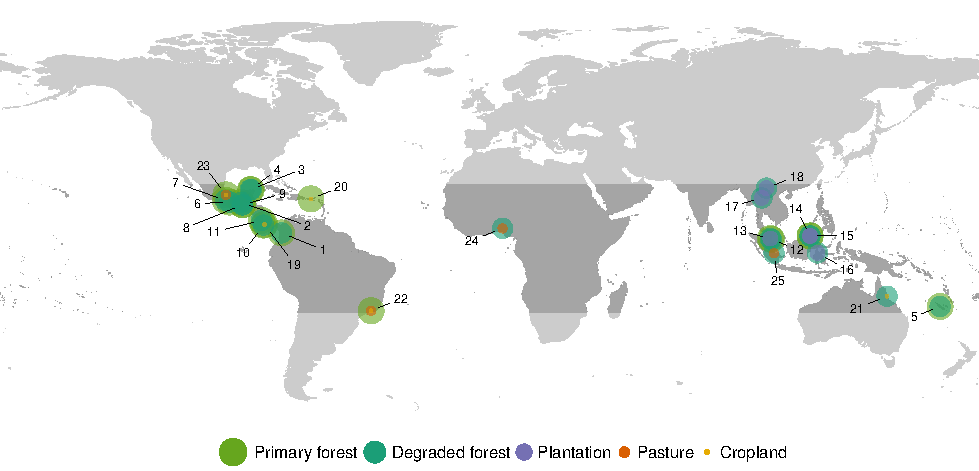
\includegraphics{./output/fig-2-1-1} 

}

\caption{Locations of the 25 studies contributing data to the
analyses. Point labels correspond to the study number in
\autoref{tab:tab-2-1}. The shading and size of concentric points
corresponds to different land-use types, to indicate the data provided
by each study.}\label{fig:fig-2-1}
\end{figure}








\begin{figure}
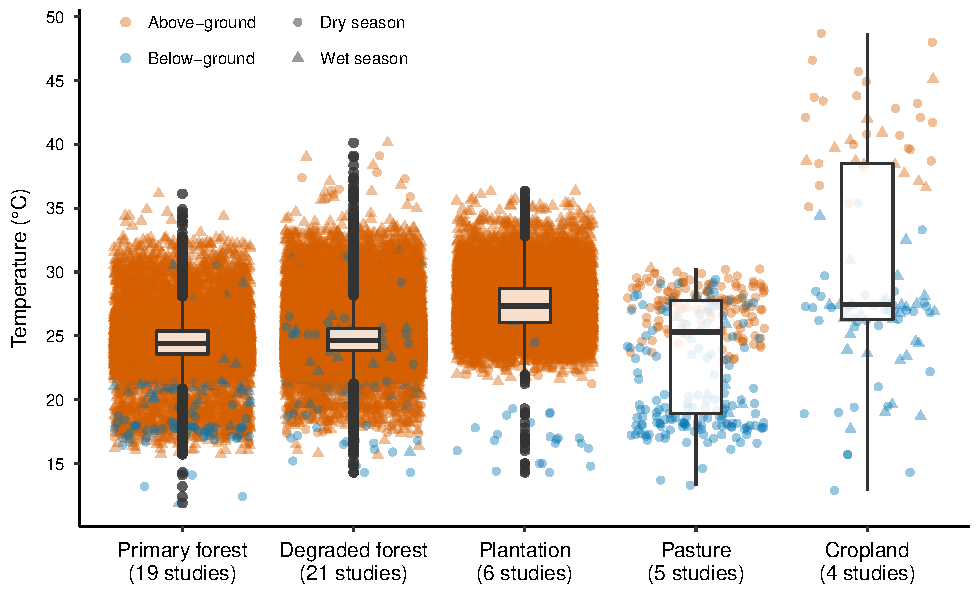
\includegraphics{./output/fig-2-2-1} \caption{Raw day-time temperature against land-use type, across all
studies contributing data to the analyses (plotted by study in
\autoref{fig:fig-A-1}). Point shading indicates temperatures measured
above-ground (orange) or below-ground (blue), and different symbols
indicate temperatures measured during the dry season (circles) or wet
season (triangles).}\label{fig:fig-2-2}
\end{figure}

\section{Results}\label{results}

In total, 25 studies met the criteria for inclusion
(\autoref{tab:tab-2-2}). Studies spanned 12 countries, across every
continent within the tropics (\autoref{fig:fig-2-1}), and provided
113,894 observations of day-time temperature (\autoref{fig:fig-2-2} and
\autoref{fig:fig-A-1}). Most observations represented either a single
temperature observation within, or mean temperature across, a single day
at the point location where measurements were taken. Six studies
reported temperature at a coarser temporal resolution (mean = 107 days;
minimum = 14 days; maximum = 183 days), and six studies reported
temperature at a coarser spatial resolution (mean = 527
m\textsuperscript{2}; minimum = 64 m\textsuperscript{2}; maximum = 1,000
m\textsuperscript{2}). The maximum elevational difference between sites
within a single study ranged from 0 to 141 m (mean = 33 m), and site
elevation was random with respect to land-use type (LMM,
Χ\textsuperscript{2} = 19.33, df = 14, P \textgreater{} 0.05;
\autoref{fig:fig-A-2}). We were also able to obtain 113,459 night-time
temperature observations (including temperature extremes) from 10
studies, plus 113,230 observations of day-time temperature extremes from
11 studies; but none of these data were collected in cropland or
pasture.

In all cases, the final model included a random slope for land-use type
(`LUT') and random intercept with respect to the identity of the study
(`studyID') from which data originated. The final model of day-time
temperature (`temp\_day') included land-use type, position relative to
ground level (`position') and season, as well as pairwise interactions
between land-use type and the latter two fixed effects:

\texttt{lmer(temp\_day\ \textasciitilde{}\ LUT*position\ +\ LUT*season\ +\ (LUT\textbar{}studyID))}

The final models of (1) night-time temperature, and temperature extremes
(minimum and maximum) (2) during the day and (3) during the night, all
had the same model structure, with land-use type as the only fixed
effect:

\texttt{lmer(temp\ \textasciitilde{}\ LUT\ +\ (LUT\textbar{}studyID))}

\begin{sidewaystable}
\renewcommand{\arraystretch}{0.85} % reduce space between rows
\setlength{\tabcolsep}{5pt} % reduce space between columns
\rowcolors{1}{lightgrey}{white}
\begin{tabular}{p{6.5cm}p{2.5cm}p{1.5cm}p{1.5cm}p{1.5cm}p{1.5cm}p{1.5cm}p{1.1cm}p{1.1cm}p{1.13cm}p{1.13cm}}\toprule \hiderowcolors
\bfseries Study & \bfseries Country & \multicolumn{5}{l}{\bfseries Land-use type} & \multicolumn{2}{l}{\bfseries Position} & \multicolumn{2}{l}{\bfseries Season}\\ 
\cmidrule(l{2pt}r{2pt}){3-7} \cmidrule(l{2pt}r{2pt}){8-9} \cmidrule(l{2pt}r{2pt}){10-11}
    & & \bfseries Primary forest & \bfseries Degraded forest & \bfseries Plantation & \bfseries Pasture & \bfseries Cropland & \bfseries Above-ground &
    \bfseries Below-ground & \bfseries Dry season & \bfseries Wet season \\ \midrule \showrowcolors
    1. \citet{gonzalez_del_pliego_unpublished}       & Colombia      & X & X &   &   &  & X &   & X & \\
    2. \citet{gonzalez-di_pierro_effects_2011}       & Mexico        & X & X &   &   &  & X &   &  & X \\
    3. \citet{goode_unpublished}                     & Mexico        & X & X &   &   &  & X &   &X & X \\
    4. \citet{goode_seed_2009}                       & Mexico        & X & X &   &   &  & X &   &X & X \\
    5. \citet{ibanez_sharp_2013}                     & New Caledonia & X & X &   &   &  & X &   &X & X \\
    6. \citet{lebrija-trejos_environmental_2011}     & Mexico        & X & X &   &   &  & X & X &X & X \\
    7. \citet{negrete-yankelevich_successional_2007} & Mexico        & X & X &   &   &  &   & X &  & X \\
    8. \citet{santos_interaccion_2011}               & Mexico        & X & X &   &   &  & X & X &  & X \\
    9. \citet{santos_insect_2012}                    & Mexico        & X & X &   &   &  & X & X &  & X \\
    10. \citet{sonnleitner_microclimatic_2009}       & Costa Rica    & X & X &   &   &  & X &   &X &   \\
    11. \citet{wood_no_2008}                         & Costa Rica    & X & X &   &   &  &   & X &  & X \\
    12. \citet{yashiro_effects_2008}                 & Malaysia      & X & X &   &   &  &   & X &X & X \\
    13. \citet{adachi_differences_2006}              & Malaysia      & X & X & X &   &  &   & X &X &   \\
    14. \citet{hardwick_aboveground_2016}            & Malaysia      & X & X & X &   &  & X &   &X & X \\
    15. \citet{hardwick_relationship_2015}           & Malaysia      & X & X & X &   &  & X &   &X & X \\
    16. \citet{klein_predatorprey_2002}              & Indonesia     &   & X & X &   &  & X &   &  & X \\
    17. \citet{wangluk_role_2013}                    & Thailand      &   & X & X &   &  &   & X &X & X \\
    18. \citet{werner_n2o_2006}                      & China         &   & X & X &   &  &   & X &X &   \\
    19. \citet{holl_factors_1999}                    & Costa Rica    & X &   &   & X &  & X & X &X &   \\
    20. \citet{liu_exotic_2002}                      & Puerto Rico   & X &   &   & X &  &   & X &X & X \\
    21. \citet{king_ants_1998}                       & Australia     &   & X &   & X &  & X & X &  & X \\
    22. \citet{badejo_response_2004}                 & Brazil        & X &   &   & X &X &   & X &  & X \\
    23. \citet{campos_response_2006}                 & Mexico        & X &   &   & X &X &   & X &X & X \\
    24. \citet{badejo_seasonal_1990}                 & Nigeria       &   & X &   &   &X &   & X &X & X \\
    25. \citet{furukawa_effect_2005}                 & Indonesia     &   & X &   &   &X & X & X &X & X \\
\bottomrule
\end{tabular}
\caption{\label{tab:tab-2-2}Summary of the 25 studies contributing data to analyses. Study number corresponds to point labels in \autoref{fig:fig-2-1}. Crosses indicate the land-use types, position(s) relative to ground level and season(s) considered by each study.}
\end{sidewaystable}

\subsection{Effect of land-use change}\label{effect-of-land-use-change}

Altered land-use types were substantially hotter than primary forest
(LMM, Χ\textsuperscript{2} = 29.49, df = 4, P \textless{} 0.001;
\autoref{tab:tab-2-3}; \autoref{fig:fig-2-3}), and the magnitude of the
warming broadly matched the intensity of vegetation change associated
with each land-use type. Thus, degraded forests in our sample were the
most similar to primary forest with an average difference of only
+1.1°C, which was not statistically significant based on 95\% confidence
intervals (\autoref{fig:fig-2-3}). By contrast, converted habitats in
our dataset -- plantation, pasture and cropland -- were, on average,
hotter than primary forest by 2.7°C, 6.2°C and 7.6°C, respectively.
Results were robust to resampling from studies that provided
disproportionate numbers of observations (\autoref{text-A-1};
\autoref{fig:fig-A-3}).

Night-time temperature, and day-time and night-time temperature
extremes, showed varying results relative to primary forest in the two
altered land-use types for which data were available: degraded forest
and plantation. In all cases, sample sizes were very limited and
confidence intervals were large, hence results should be interpreted
with caution. Night-time temperature in degraded forest and plantation
did not differ from that of primary forest (LMM, Χ\textsuperscript{2} =
2.09, df = 2, P \textgreater{} 0.05; \autoref{fig:fig-A-4}), and neither
did night-time minimum temperature (LMM, Χ\textsuperscript{2} = 2.31, df
= 2, P \textgreater{} 0.05; \autoref{fig:fig-A-5}d). Maximum night-time
temperature was slightly higher overall in degraded forest and
plantation compared to primary forest (LMM, Χ\textsuperscript{2} = 6.35,
df = 2, P \textless{} 0.05; \autoref{fig:fig-A-5}c), although pairwise
differences were not statistically significant according to 95\%
confidence intervals. There was no difference between primary forest and
degraded forest and plantation in terms of day-time maximum temperature
(LMM, Χ\textsuperscript{2} = 4.87, df = 2, P \textgreater{} 0.05;
\autoref{fig:fig-A-5}a), or day-time minimum temperature (LMM,
Χ\textsuperscript{2} = 4.60, df = 2, P \textgreater{} 0.05;
\autoref{fig:fig-A-5}b).















\begin{figure}
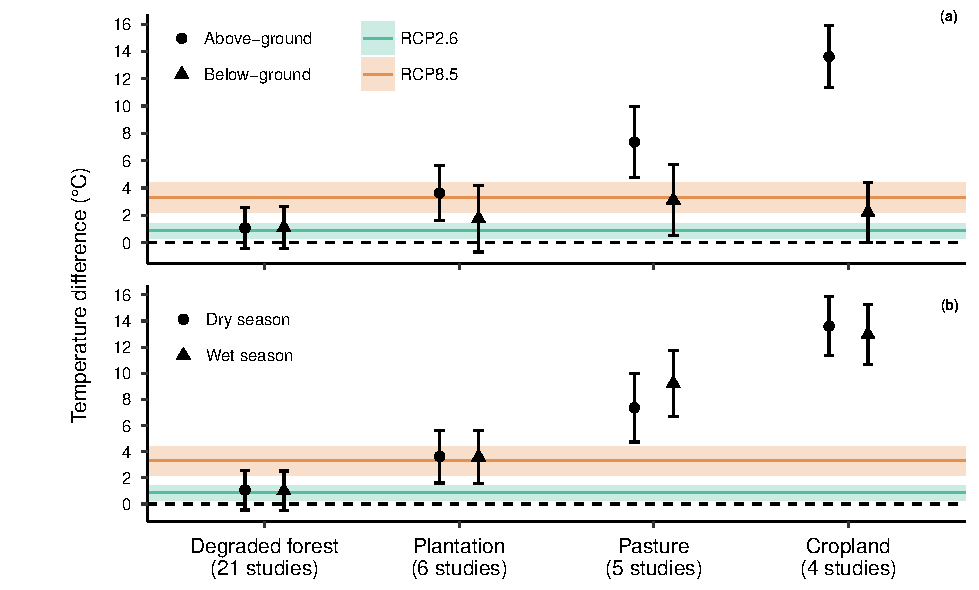
\includegraphics{./output/fig-2-3-1} \caption{Model estimates of local day-time temperature in altered
land-use types relative to primary forest (depicted by the black dashed
line). In panel (a), different symbols denote position relative to the
ground (above-or below-ground), and the season is held at the reference
level (dry season). In panel (b), different symbols denote the season
(dry or wet), and the position relative to the ground is held at the
reference level (above-ground). Error bars are 95\% confidence
intervals. Solid lines indicate projected warming in the tropics for the
period 2081--2100 compared to the period 1986--2005, as a result of
global climate change \citep{ipcc_climate_2013}. Shaded bands indicate
5\%--95\% ranges from the distribution of the climate model ensemble.
Colors represent the lowest and highest warming scenarios (RCP2.6 and
RCP8.5, respectively).}\label{fig:fig-2-3}
\end{figure}

\subsection{Above- versus
below-ground}\label{above--versus-below-ground}

The warming effect of land-use change was much stronger above-ground
than below-ground (LMM, Χ\textsuperscript{2} = 1115, df = 4, P
\textless{} 0.001; \autoref{tab:tab-2-3}; \autoref{fig:fig-2-3}a). The
average difference between the local temperature of altered land-use
types and primary forest was greater if measured above-ground rather
than below-ground, by 1.9°C in plantation, 4.3°C in pasture, and 11.4°C
in cropland. In degraded forest, the temperature relative to primary
forest was very similar above- (+1°C) and below-ground (+1.1°C).
Notably, the buffering effect below ground was so great that any
difference between primary forest and impacted land uses was effectively
negated in all land-use types but pasture (based on 95\% confidence
intervals; \autoref{fig:fig-2-3}a).

\subsection{Dry versus wet season}\label{dry-versus-wet-season}

Seasonality had some influence on the relationship between land-use
change and temperature (LMM, Χ\textsuperscript{2} = 14.91, df = 4, P
\textless{} 0.01; \autoref{tab:tab-2-3}; \autoref{fig:fig-2-3}b), but
the direction of the interaction varied by land-use type, and in all
cases the effect size was very small. In degraded forest and plantation,
seasonality had no appreciable effect on temperature relative to primary
forest (dry vs.~wet season: +0.1°C in both degraded forest and
plantation). In contrast, the temperature difference between pasture and
primary forest was 1.9°C greater in the wet versus dry season, while in
cropland the differential was 0.6°C greater in the dry versus wet
season.

\begin{sidewaystable}
\renewcommand{\arraystretch}{1.1} % reduce space between rows
\setlength{\tabcolsep}{5pt} % reduce space between columns
\begin{center}
\begin{tabular}{p{3cm}p{1.3cm}p{1.3cm}p{1.3cm}p{1.3cm}p{1.3cm}p{1.3cm}p{1.3cm}p{1.3cm}p{1.5cm}p{1.3cm}p{1.3cm}p{1.5cm}}\toprule
    \bfseries Land-use type & \bfseries Position & \bfseries Season & \bfseries Temp. vs. PF & \bfseries Lower CI & \bfseries Upper CI & \bfseries LUT mean & \bfseries Position & \bfseries Position mean & \bfseries Position effect (AG-BG) & \bfseries Season & \bfseries Season mean & \bfseries Season effect (dry-wet) \\
    \hline
    Degraded forest & AG & Dry & 1.1 & -0.5 & 2.6 &                     & AG & 1   &                      & Dry & 1.1 &                      \\
                    &    & Wet & 1   & -0.5 & 2.5 &                     &    &     &                      & Wet & 1   &                      \\
                    & BG & Dry & 1.1 & -0.4 & 2.6 &                     & BG & 1.1 &                      &     &     &                      \\
                    &    & Wet & 1   & -0.5 & 2.6 &\multirow{-4}{*}{1.1}&    &     &\multirow{-4}{*}{0.1} &     &     &\multirow{-4}{*}{0.1} \\\rowcolor{lightgrey}
    Plantation      & AG & Dry & 3.6 & 1.6  & 5.6 &                     & AG & 3.6 &                      & Dry & 2.7 &                      \\\rowcolor{lightgrey}
                    &    & Wet & 3.6 & 1.6  & 5.6 &                     &    &     &                      & Wet & 2.6 &                      \\\rowcolor{lightgrey}
                    & BG & Dry & 1.8 & -0.7 & 4.2 &                     & BG & 1.7 &                      &     &     &                      \\\rowcolor{lightgrey}
                    &    & Wet & 1.7 & -0.7 & 4.2 &\multirow{-4}{*}{2.7}&    &     &\multirow{-4}{*}{1.9} &     &     &\multirow{-4}{*}{0.1} \\
    Pasture         & AG & Dry & 7.4 & 4.7  & 10  &                     & AG & 8.3 &                      & Dry & 5.2 &                      \\
                    &    & Wet & 9.2 & 6.7  & 11.8&                     &    &     &                      & Wet & 7.1 &                      \\
                    & BG & Dry & 3.1 & 0.5  & 5.7 &                     & BG & 4   &                      &     &     &                      \\
                    &    & Wet & 5   & 2.4  & 7.5 &\multirow{-4}{*}{6.2}&    &     &\multirow{-4}{*}{4.3} &     &     &\multirow{-4}{*}{-1.9}\\\rowcolor{lightgrey}
    Cropland        & AG & Dry & 13.6& 11.3 & 15.9&                     & AG & 13.3&                      & Dry & 7.9 &                      \\\rowcolor{lightgrey}
                    &    & Wet & 13  & 10.7 & 15.2&                     &    &     &                      & Wet & 7.3 &                      \\\rowcolor{lightgrey}
                    & BG & Dry & 2.2 & 0    & 4.4 &                     & BG & 1.9 &                      &     &     &                      \\\rowcolor{lightgrey}
                    &    & Wet & 1.6 &-0.6  & 3.7 &\multirow{-4}{*}{7.6}&    &     &\multirow{-4}{*}{11.4}&     &     &\multirow{-4}{*}{0.6} \\
\bottomrule
\end{tabular}
\end{center}
\caption{\label{tab:tab-2-3}Model estimates (with 95\% confidence intervals) of local day-time temperature in altered land-use types relative to primary forest (PF), with respect to position relative to ground level and season. 'Position effect' refers to the difference between temperature measured above-ground (AG) versus below-ground (BG), averaged across seasons. 'Season effect' refers to the difference between temperature measured in the dry season versus the wet season, averaged across positions. All figures are quoted in \degree C.}
\end{sidewaystable}

\section{Discussion}\label{discussion}

Our results show that land-use change increases local temperature in the
tropics (\autoref{fig:fig-2-3}). In all conditions where this
relationship was evident, the temperature rise due to land-use change
exceeded that predicted for the tropics by the end of the 21st Century
under the minimum climate warming scenario \citep[+0.9°C in
RCP2.6;][]{ipcc_climate_2013}, and frequently also exceeded the maximum
warming scenario \citep[+3.3°C in RCP8.5;][]{ipcc_climate_2013}.
Previous studies show that land-use change tends to increase local
temperature
\citep[e.g.][]{findell_modeled_2007, loarie_velocity_2009, davin_climatic_2010, luskin_microclimate_2011, ramdani_local_2014, tuff_framework_2016}
but this is the first study, to our knowledge, that demonstrates this
effect across many locations in the tropics at a site-level resolution
(\textless{} 1 ha), considering multiple modes of land-use change
concurrently, and comparing the relationship above- and below-ground and
between wet and dry seasons.

\subsection{Thermal differences between land-use
types}\label{thermal-differences-between-land-use-types}

Human-impacted land-use types are likely hotter than intact primary
forest because of changes in evapotranspiration and the amount of solar
radiation reaching the Earth's surface
\citep{oke_boundary_1987, findell_modeled_2007, davin_climatic_2010}.
Degradation and deforestation cause a lowering and thinning of the
canopy, and reduction in rooting depth, leaf area index and surface
roughness, all of which reduce evapotranspiration
\citep{okuda_effect_2003, snyder_analyzing_2004, kumar_effects_2005, findell_modeled_2007, davin_climatic_2010, hardwick_relationship_2015},
and thereby increase temperature
\citep{oke_boundary_1987, foley_global_2005}. Changes to canopy
architecture and a reduction in the number of sub-canopy vegetation
strata also cause warming by increasing the amount of solar radiation
reaching the ground \citep{oke_boundary_1987, murcia_edge_1995}. Our
land use categories encompass a spectrum of vegetation change, from
relatively little change in degraded forests (where some trees and a
closed canopy are maintained) to maximal change in pasture and cropland
(where trees are replaced with herbaceous plants). Accordingly,
degradation had the smallest average effect (+1.1°C), followed by
plantation (+2.7°C), and then pasture (+6.2°C) and cropland (+7.6°C). We
expected that the same mechanisms underlying the warming effect of
land-use change would also result in increased day-time temperature
extremes and decreased night-time temperatures in altered land-use
types, relative to primary forest
\citep{oke_boundary_1987, chen_growing-season_1995}. Unfortunately, the
data available were very limited, including only three of the five
land-use types (primary forest, degraded forest and plantation), and
resulting in extremely large confidence intervals (\autoref{fig:fig-A-3}
and S4). We urge caution when interpreting our results, which suggested
either no effect or an extremely weak effect of land-use change on
temperature extremes and night-time temperature; clearly more data are
needed to reliably test these relationships.

\subsection{Interaction with position relative to ground level and
seasonality}\label{interaction-with-position-relative-to-ground-level-and-seasonality}

We found that local warming effects of tropical land-use change are
negated below-ground, despite the strength of the relationship
above-ground (\autoref{tab:tab-2-3}; \autoref{fig:fig-2-3}a). This can
largely be attributed to the higher specific heat capacity of soil
compared to air \citep{oke_boundary_1987}. Greater availability of water
may also play a role, permitting thermal energy to be dissipated through
the evaporation of water rather than increasing temperature
\citep{oke_boundary_1987, davin_climatic_2010, christidis_role_2013}. We
expected the latter effect to result in increased buffering during the
wet season \citep[cf.][]{findell_modeled_2007, davin_climatic_2010}, but
instead we found that seasonality had a very limited influence on
temperature relative to primary forest (\autoref{tab:tab-2-3};
\autoref{fig:fig-2-3}b). The strongest influence was in pasture, where
the effect of land-use change was greater in the wet season. Potentially
longer grass in pasture in the wet season could decrease albedo compared
to pale exposed soil in the dry season, while the same pattern could be
avoided in cropland through dry season irrigation. That said, pasture
and cropland had the least data of all land-use types, and we advise
that these results be interpreted with caution.

\subsection{Implications for
biodiversity}\label{implications-for-biodiversity}

For tropical biodiversity, there are several key implications of our
findings. Firstly, forest species persisting through forest conversion
have already experienced thermal change similar, if not greater, in
magnitude to that predicted by global climate change
\citep{ipcc_climate_2013}. Historically the tropics have experienced
relatively stable climatic conditions \citep{mora_projected_2013} and
tropical species possess narrow thermal niches, with many already
occupying the upper bounds of that niche
\citep{deutsch_impacts_2008, tewksbury_putting_2008, freeman_rapid_2014, sunday_thermal-safety_2014}.
Dispersal towards more favourable climatic conditions is limited by low
dispersal ability \citep{van_houtan_dispersal_2007}, a scarcity of
suitable destinations \citep{colwell_global_2008}, and the necessity to
pass through an increasingly hostile land-use matrix to reach target
habitat
\citep{thomas_extinction_2004, brook_synergies_2008, scriven_protected_2015}.
There is already some evidence that higher temperatures in the tropics
are associated with lower species abundance \citep[e.g.~for
arthropods:][]{foster_establishing_2011}, and there are also fitness
costs associated with long-term persistence in suboptimal climatic
conditions \citep{du_plessis_costs_2012, gunderson_conceptual_2016}.
Without any further temperature change some species persisting in
converted environments may already be committed to extinction,
particularly species that are unable to utilise microhabitats with
favourable microclimates
\citep{scheffers_microhabitats_2014-1, gonzalez_del_pliego_thermally_2016}.
Under predicted climate change, increasing average temperature and the
increasing frequency and intensity of droughts
\citep{chou_changes_2012, ipcc_climate_2013} will likely push many
species beyond their upper thermal limits, especially in heavily
degraded or converted habitats.

That said, we find several circumstances where warming through land-use
change is mitigated. Degraded forests were not significantly hotter than
primary forests (according to 95\% confidence intervals;
\autoref{fig:fig-2-3}). This is encouraging because degraded forests are
likely to become the most widespread land-use type in future
\citep{hurtt_harmonization_2011}, and many studies have demonstrated
their capacity to retain species of conservation concern
\citep{edwards_degraded_2011, gibson_primary_2011, putz_sustaining_2012, edwards_maintaining_2014}.
For all altered land-use types, the warming effect was limited
below-ground, highlighting a crucial thermal refuge for species that are
able to occupy the soil, and suggesting that above-ground microhabitats,
such as deadwood and epiphytes, might fulfil a similar role
\citep{scheffers_microhabitats_2014-1, gonzalez_del_pliego_thermally_2016}.
Thermal refugia may not be a permanent solution for avoiding climate
change, and sensitive species may find that even relatively cold
microhabitats are still too hot (e.g.~below-ground in pasture was 4°C
warmer than primary forest; \autoref{tab:tab-2-3};
\autoref{fig:fig-2-3}), but refugia could at least provide species with
more time to respond to suboptimal climatic conditions
\citep{hannah_fine-grain_2014}.

\subsection{Caveats and knowledge
gaps}\label{caveats-and-knowledge-gaps}

By collating site-level data reported from the literature, we were able
to achieve high geographical coverage and fine spatial resolution that
is lacking in previous studies, but this technique is biased by the
availability of data towards particular regions and land-use types
(\autoref{fig:fig-2-1}), and relies heavily on substituting space for
time, which can misrepresent anthropogenic impacts
\citep{franca_space-for-time_2016}. In particular, there was only one
study located in Africa, and Southeast Asian studies provided all of the
plantation data and no cropland data. Future research should seek to
explicitly consider how tropical land-use change affects: vegetation
structure \citep[e.g.~using Leaf Area Index
cf.][]{hardwick_relationship_2015}, relative humidity
\citep{luskin_microclimate_2011, ewers_fragmentation_2013}, nocturnal
climatic conditions
\citep{chen_growing-season_1995, dubreuil_impact_2011}, extremes of
temperature \citep{christidis_role_2013}, and rates of temperature
change \citep{scheffers_microhabitats_2014-1}; preferably at a range of
spatiotemporal scales \citep{wiens_matching_2010} and with a
standardised methodology to simplify comparisons across studies.

\subsection{Conclusions}\label{conclusions}

Our study confirms that tropical land-use change leads to warming at a
local scale (\textless{} 1 ha) across the tropics, of a magnitude
comparable to that predicted from global climate change. We find
pantropical evidence that the effects of land-use change on temperature
are ameliorated below-ground, and absent in degraded forests. Many
studies collect site-level climate data, and through sharing of these
data and collaboration between scientific disciplines, there is much
that can be done to integrate theoretical and empirical understanding of
the processes that govern climate at different scales. This will greatly
advance our knowledge of potential synergies between two of the greatest
drivers of biodiversity loss -- land-use change and climate change --
and highlight mitigating factors, such as thermal microrefugia, which
could be a pragmatic focus for conservation management.

\section{Data availability and R
code}\label{data-availability-and-r-code}

The collated dataset can be found on Dryad
(\url{https://doi.org/10.5061/dryad.g4000}). Note that in many cases
these data were aggregated for analyses. For finer resolution data
please refer to the original data sources. R functions used to estimate
time of sunset and sunrise can be downloaded from GitHub
(\url{https://github.com/rasenior/SolarCalc}).

\section{Acknowledgements}\label{acknowledgements-1}

We thank the following people for providing temperature data: Julieta
Benítez Malvido, Stephen Hardwick, Karen Holl, Thomas Ibanez, and
Bráulio Santos. A considerable amount of data was provided by the
Stability of Altered Forest Ecosystem (SAFE) Project, for which we
acknowledge their primary sponsor: the Sime Darby Foundation. We thank
Tim Newbold for statistical advice. R.A.S. was funded by a NERC
studentship through the ACCE (Adapting to the Challenges of a Changing
Environment) Doctoral Training Partnership (Grant No. NE/L002450/1);
P.G. was supported by CONACyT, Scholarship 359063. We also thank two
anonymous referees for their comments, which greatly improved the
manuscript.

\chapter{A framework for quantifying fine-scale thermal heterogeneity in
the
field}\label{a-framework-for-quantifying-fine-scale-thermal-heterogeneity-in-the-field}

\begin{figure}[!htb]
\centering
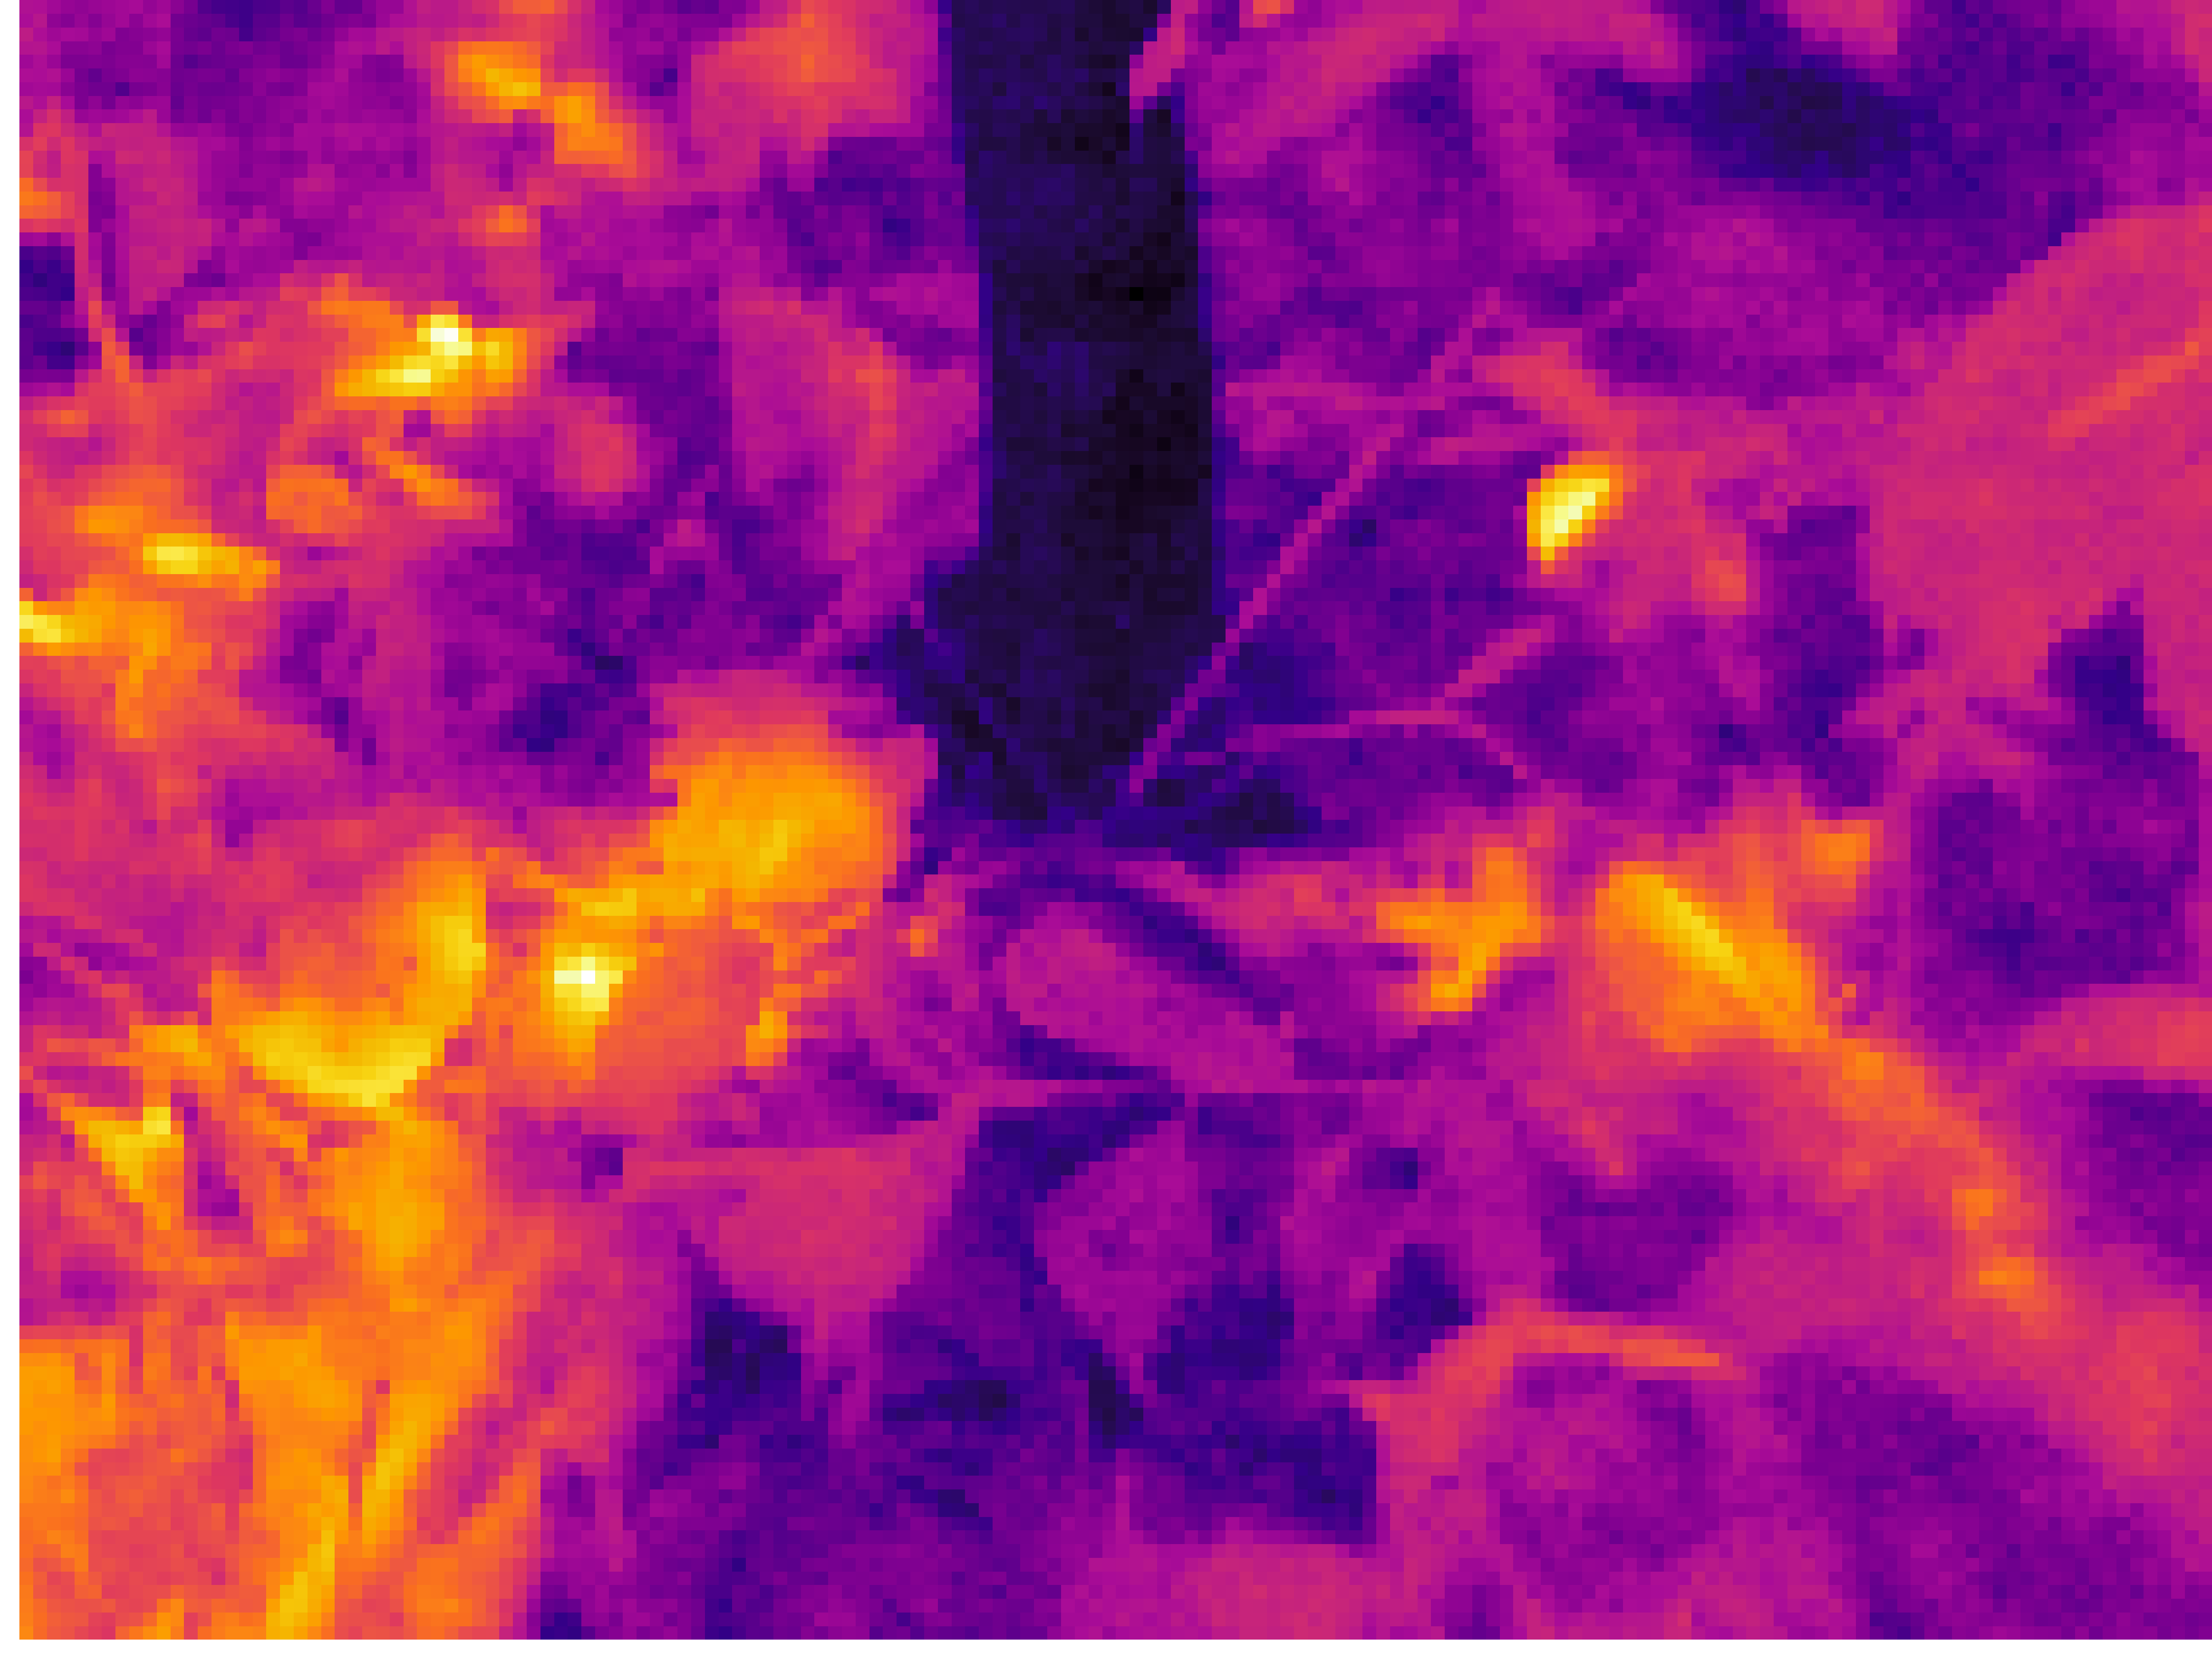
\includegraphics[width=15cm]{pics/Themal-image1.png}
\caption*{Thermal image of rainforest floor.}
\end{figure}

\pagebreak

\section{Abstract}\label{abstract-2}

Variation in temperature at a fine spatial scale creates critically
important microclimates for many organisms. Quantifying thermal
heterogeneity at this scale is challenging, and has so far been largely
restricted to the use of dataloggers. Thermography is becoming an
increasingly affordable and viable alternative. A single thermal photo
contains thousands of spatially-explicit surface temperature
measurements, and is therefore ideal for rapidly assessing fine-scale
spatial temperature variation, including the surfaces within a few cms
of which most organisms actually experience temperature. Both the
technology and data have been underexploited in terrestrial ecology, in
part because there is limited technical support for processing and
interpreting these data. Here we present a simple R package for batch
extracting and converting data from FLIR thermal cameras, and for
quantifying thermal heterogeneity in gridded temperature data more
generally. We apply this framework to investigate how forest structure
affects thermal heterogeneity in primary forests in Borneo, using both
(1) fine-scale FLIR thermal images collected in the field, and (2)
remotely-sensed thermal data. Our various metrics of thermal
heterogeneity show\ldots{}. Our framework simplifies the process of
getting data into a usable format, and demonstrates that\ldots{} The
importance of microclimates to species' ecology necessitates an
efficient methodology for sampling thermal heterogeneity at the relevant
spatial scale; streamlining data processing and analysis -- as we do
here -- is a major part of this.

\section{Introduction}\label{introduction-1}

\begin{itemize}
\tightlist
\item
  A key mechanism by which organisms will respond to future climate
  change is adaptation \emph{in situ} \citep{hannah_fine-grain_2014}.
\item
  Many organisms in structurally complex tropical rainforests respond to
  extremes of heat by exploiting fine-scale (mm to m) thermal
  heterogeneity
  \citep{scheffers_microhabitats_2014, gonzalez_del_pliego_thermally_2016}.
\item
  The ability of many tropical organisms to adaptively respond to
  climate change is therefore critically dependent on variation in
  temperature at this scale.
\item
  Previously, fine-scale thermal heterogeneity was captured using
  temperature dataloggers. Dataloggers suspended in the understorey
  record air temperature that has been equilibrated by the movement of
  air masses, and thus represents forest temperature at a local scale
  \citep[m to
  ha;][]{scheffers_microhabitats_2014, gonzalez_del_pliego_thermally_2016}.
  Dataloggers placed inside microhabitats -- such as tree holes and
  epiphytes -- record air temperature at the finest spatial scale (mm to
  cm), and we know from these studies that the cool microclimates inside
  these microhabitats are able to thermally buffer inhabitant frogs and
  lizards from temperature change at a local scale.
\item
  The use of temperature dataloggers has clearly been instrumental in
  advancing this field. However, dataloggers can only record the air
  temperature in their immediate vicinity, and must therefore be highly
  replicated in space (and in a variety of microhabitats) to adequately
  quantify spatial temperature variation. The number of dataloggers
  available to the user imposes a financial and logistical limit on the
  spatial representativeness of sampling. Furthermore, the vast majority
  of terrestrial organisms are very small, flat, or thigmothermic
  (thermoregulate via direct contact with a surface), and therefore
  surface temperature is often more relevant than air temperature
  \citep[e.g.][]{kaspari_thermal_2015}.
\item
  Technological advances mean that the use of thermal cameras is
  increasingly affordable and practical
  \citep{scheffers_extreme_2017, faye_toolbox_2016}.
\item
  Thermal photos are ideal for capturing fine-scale surface temperature
  in tropical rainforests. Each photo provides thousands of
  spatially-explicit temperature measurements at the mm-cm scale.
  However, both the technology itself and the data provided have thus
  far been underexploited. Owing to the novelty of the methodology,
  there is little guidance for what metrics ought to be calculated and
  how.
\item
  \citet{faye_toolbox_2016} provide an excellent starting point from
  which to formulate such a framework. Using standard RGB images in
  combination with thermal images, collected using an unmanned aerial
  vehicle (UAV), Faye et al. demonstrate how this technology can be used
  to compare thermal heterogeneity between different surfaces (in this
  case, bare soil versus crop surface), and suggest metrics that they
  consider to be most appropriate to capture different facets of thermal
  heterogeneity.
\item
  Their toolbox, however, does not immediately facilitate a general
  assessment of thermal heterogeneity using photos collected in the
  field. While the use of UAVs in the tropics is indeed becoming more
  feasible and affordable \citep{sanchez-azofeifa_twenty-first_2017},
  for the foreseeable future it is likely that thermography in tropical
  rainforests will most commonly consist of manually collected thermal
  photos.
\item
  Additionally, while \citet{faye_toolbox_2016} and
  \citet{scheffers_extreme_2017} provide introductory R scripts to
  facilitate the processing of thermal photos, there remains little
  technical support and guidance for ecologists for what is, in reality,
  an otherwise difficult and time-consuming element of any study seeking
  to utilise this technology.
\item
  The development of the \texttt{Thermimage} package in R has
  considerably eased the extraction and conversion of raw data from FLIR
  thermal cameras, but this package does not directly facilitate batch
  processing and does not calculate (nor suggest) what metrics are most
  appropriate to quantify thermal heterogeneity from thermal images.
\item
  In this study, we introduce a developmental R package --
  \texttt{thermstats} -- for batch extraction, processing and analysing
  images from FLIR thermal cameras, extending the functionality of the
  \texttt{Thermimage} package. We outline the utility of our package by
  comparing metrics of thermal heterogeneity over time and varying
  forest structure. In addition, we demonstrate that our functions for
  quantifying thermal heterogeneity can also be applied to other kinds
  of thermal image, including those at a coarser spatial scale.
\end{itemize}

\section{Methods}\label{methods-1}

\subsection{Step 1: Data collection}\label{step-1-data-collection}

\begin{itemize}
\tightlist
\item
  Key technical considerations for data collection

  \begin{itemize}
  \tightlist
  \item
    Environmental parameters:

    \begin{itemize}
    \tightlist
    \item
      Atmospheric temperature
    \item
      Relative humidity
    \item
      Object distance
    \item
      Emissivity
    \end{itemize}
  \end{itemize}
\item
  Camera calibration
\item
  Format of FLIR thermal images (e.g.~for a model E40: 160 x 120 pixels)
\end{itemize}

\subsection{Step 2: Data extraction}\label{step-2-data-extraction}

\begin{itemize}
\tightlist
\item
  Requires ExifTool installation (freely available:
  \url{https://sno.phy.queensu.ca/~phil/exiftool/})
\item
  Batch extract data from thermal jpeg files using
  \texttt{batch\_extract} function in \texttt{thermstats}

  \begin{itemize}
  \tightlist
  \item
    Batch implementation of \texttt{readflirJPG} in \texttt{Thermimage}
    package
  \end{itemize}
\end{itemize}

\subsection{Step 3: Conversion of raw
data}\label{step-3-conversion-of-raw-data}

\begin{itemize}
\tightlist
\item
  Describe format of the raw data
\item
  Retrieve camera calibration constants using \texttt{flirsettings} in
  \texttt{Thermimage} package
\item
  Specify environmental parameters (see Step 1)
\item
  Batch convert raw data to temperature in °C using
  \texttt{batch\_convert} in \texttt{thermstats}

  \begin{itemize}
  \tightlist
  \item
    Batch implementation of \texttt{raw2temp} in \texttt{Thermimage}
    package
  \end{itemize}
\end{itemize}

\subsection{Step 4: Calculate metrics of thermal
hetereogeneity}\label{step-4-calculate-metrics-of-thermal-hetereogeneity}

\begin{itemize}
\tightlist
\item
  Function \texttt{stats\_by\_group} in \texttt{thermstats} calculates
  statistics across multiple photos within a specified grouping

  \begin{itemize}
  \tightlist
  \item
    Based on the assumption that multiple photos are required at each
    sampling location to adequately represent spatial variation in
    temperature\ldots{}
  \item
    \ldots{}but also works if the photo itself is the unit of
    replication
  \end{itemize}
\item
  Calculates summary statistics (specified by the user) across all
  pixels of all photos within the group, e.g.:

  \begin{itemize}
  \tightlist
  \item
    Mean
  \item
    Standard deviation
  \item
    Median
  \item
    Percentiles
  \item
    Kurtosis and skewness
  \item
    Diversity indices
  \end{itemize}
\item
  Identifies hot and cold patches using Getis-Ord local statistic
  \citep{getis_local_1996}, via function \texttt{get\_patches}

  \begin{itemize}
  \tightlist
  \item
    Implements \texttt{localG} function from \texttt{spdep} package
  \item
    Option to return patches as a \texttt{SpatialPolygonsDataFrame} and
    plot using \texttt{plot\_patches}
  \end{itemize}
\item
  Calculates spatial statistics of hot and cold patches:

  \begin{itemize}
  \tightlist
  \item
    Patch area (number of pixels)
  \item
    Patch density (number of hot/cold patches per m\textsuperscript{2})
  \item
    Patch configuration (Aggregation Index of hot/cold patches)
  \end{itemize}
\end{itemize}

\subsection{Case studies}\label{case-studies}

\begin{enumerate}
\def\labelenumi{\arabic{enumi}.}
\tightlist
\item
  How does forest structure affect fine-scale thermal heterogeneity?

  \begin{itemize}
  \tightlist
  \item
    Expect that more open and less structurally complex forest would be
    more homogenous (e.g.~narrower temperature range, smaller and fewer
    cold patches that are highly clustered, but more hot patches)
  \end{itemize}
\item
  How does time of day affect fine-scale thermal heterogeneity?

  \begin{itemize}
  \tightlist
  \item
    Midday is when ambient temperature is highest, and thus
    heterogeneity is most important for organisms seeking to avoid
    extremes of heat (especially important under climate change)
  \item
    Thermal heterogeneity will increase from dawn to midday as hot and
    cold spots increasingly deviate from the average temperature
  \item
    The effect will be more extreme in forests with a more complex
    physical structure, with a greater variety of radiative properties
    across the components of the surface
  \end{itemize}
\end{enumerate}

\subsubsection{Field study}\label{field-study}

\begin{itemize}
\tightlist
\item
  Description of study area and sampling design for collecting thermal
  images with FLIR E40 camera in 2014 and 2015
\item
  Description of forest structure variables

  \begin{itemize}
  \tightlist
  \item
    Tree stand basal area and its coefficient of variation
  \item
    Sapling stand basal area and its coefficient of variation
  \item
    Proportion of trees that were dipterocarps
  \item
    \% canopy cover
  \item
    \% veg. cover at different strata
  \end{itemize}
\item
  Statistical analyses

  \begin{itemize}
  \tightlist
  \item
    Generalized Additive Mixed Models of each metric of thermal
    heterogeneity against forest structure and time of day
  \item
    Random intercept for plot nested in site
  \end{itemize}
\end{itemize}

\subsubsection{Remote study}\label{remote-study}

\begin{itemize}
\tightlist
\item
  Example of applying same metrics to coarser scale thermal data
\item
  Description of the thermal data and forest structure data

  \begin{itemize}
  \tightlist
  \item
    Note that only forest structure is available here, not time of day
  \item
    Forest structure data from LiDAR, including canopy height and canopy
    openness
  \end{itemize}
\item
  Statistical analyses

  \begin{itemize}
  \tightlist
  \item
    Linear Models of each metric of thermal heterogeneity against forest
    structure
  \end{itemize}
\end{itemize}

\section{Results}\label{results-1}

\subsection{Frequency distribution of
temperature}\label{frequency-distribution-of-temperature}

\begin{itemize}
\tightlist
\item
  (Response variables include 5\textsuperscript{th} and
  95\textsuperscript{th} percentiles, the range between them, Shannon
  Diversity Index and Simpson Diversity Index)
\item
  Impact of time of day and forest structure

  \begin{itemize}
  \tightlist
  \item
    Field study only
  \end{itemize}
\item
  Impact of forest structure

  \begin{itemize}
  \tightlist
  \item
    Field \emph{and} remote study
  \end{itemize}
\end{itemize}

\subsection{Spatial distribution of
temperature}\label{spatial-distribution-of-temperature}

\begin{itemize}
\tightlist
\item
  (Response variables include patch area, patch density and patch
  Aggregation Index, for hot and cold patches separately)
\item
  Impact of time of day and forest structure

  \begin{itemize}
  \tightlist
  \item
    Field study only
  \end{itemize}
\item
  Impact of forest structure

  \begin{itemize}
  \tightlist
  \item
    Field \emph{and} remote study
  \end{itemize}
\item
  Example field study results:

  \begin{itemize}
  \tightlist
  \item
    From dawn onwards the average area of hot patches increased slightly
    towards a plateau around midday (GAMM, F = 28.02, P \textless{}
    0.001; \autoref{fig:fig-3-1}a). This was countered by a fall in the
    density of hot patches (per m\textsuperscript{2}), which reached its
    minimum value at around midday (GAMM, F = 28.02, P \textless{}
    0.001; \autoref{fig:fig-3-1}b). Forest structure (measured by tree
    stand basal area; m\textsuperscript{2}/ha), however, did not affect
    hot patch area (GAMM, F = 0.029, P \textgreater{} 0.05) or density
    (GAMM, F = 0.101, P \textgreater{} 0.05).
  \end{itemize}
\end{itemize}










\begin{figure}
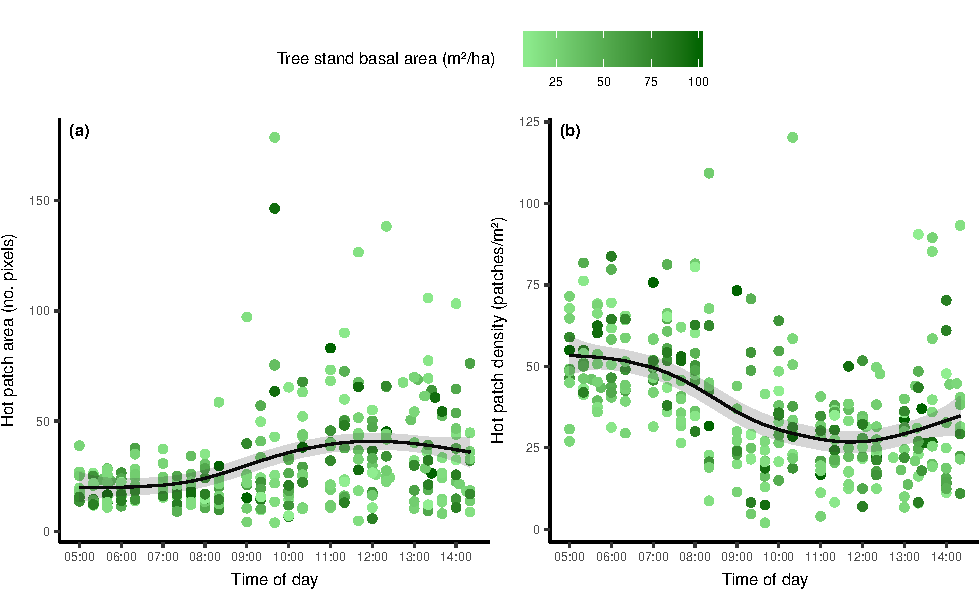
\includegraphics{./output/fig-3-1-1} \caption{The influence of time and forest structure (measured as
tree stand basal area; m\textsuperscript{2}/ha) on the average area of
hot patches (a) and the density of hot patches
(patches/m\textsuperscript{2}; b). Points are shaded according to forest
structure, from simpler, more open forests in light green to more
complex and closed forests in dark green. Fitted values for patch
characteristics against time of day are depicted by the black line, with
a grey band for the 95\% confidence intervals.}\label{fig:fig-3-1}
\end{figure}

\section{Discussion}\label{discussion-1}

\begin{itemize}
\tightlist
\item
  Our developmental R package offers users a structured and simple way
  to process thermal photos, tailored towards photos collected using a
  FLIR camera but with applicability for other kinds of thermal photos
\item
  There are various metrics of thermal heterogeneity that we consider to
  be of prime biological importance, including our novel application of
  hot spot analysis

  \begin{itemize}
  \tightlist
  \item
    Frequency distribution statistics describe the overall availability
    of different temperatures

    \begin{itemize}
    \tightlist
    \item
      Important for meeting the thermal requirements of a variety of
      species
    \item
      Temperature extremes are particularly important for buffering
      organisms against temperature change at a coarser spatial scale
    \end{itemize}
  \item
    Hot spot analysis allows us to identify spatial clusters of
    temperature extremes, the characteristics of which (e.g.~area,
    density and configuration) determines the ease with which they can
    be utilised by different organisms
  \item
    Reiterate that these metrics are not readily captured by existing
    methodologies i.e.~dataloggers
  \end{itemize}
\item
  Discuss case studies

  \begin{itemize}
  \tightlist
  \item
    Compare field and remote study results
  \item
    Over the course of day, changes in temperature at a coarser scale
    translate to changes in fine-scale thermal heterogeneity, which we
    are able to detect using our various metrics, which capture
    different facets of temperature variation.
  \end{itemize}
\item
  Discuss the limitations of thermal cameras (best used in combination
  with dataloggers)

  \begin{itemize}
  \tightlist
  \item
    Cannot directly capture sub-surface temperatures (though surface
    temperature is influenced by sub-surface temperature)
  \item
    Inferior to dataloggers for capturing temporal variation in
    temperature
  \item
    Still somewhat expensive and sensitive to heat and humidity
  \item
    Ensure that the camera is calibrated and environmental parameters
    are recorded
  \end{itemize}
\end{itemize}

\subsection{Summary}\label{summary}

\begin{itemize}
\tightlist
\item
  Thermal heterogeneity is crucial for thermoregulation by many species,
  and increasingly so under climate change. Our package and framework
  provides support and guidance for researchers, enabling them to
  address key issues in ecology with the help of increasingly efficient
  technology.
\item
  We provide a fully-reproducible example of how our approach can be
  used to quantify thermal heterogeneity in tropical forests using data
  at a fine spatial scale, collected using a FLIR thermal camera. We
  also show how our metrics can be calculated for other kinds of thermal
  data, such as those collected at a coarser spatial scale.
\end{itemize}

\chapter{Tropical forests are thermally buffered despite intensive
selective
logging}\label{tropical-forests-are-thermally-buffered-despite-intensive-selective-logging}

\begin{figure}[!htb]
\centering
\includegraphics[width=13cm]{pics/Bornean_tree_hole_frog.jpg}
\caption*{Bornean tree hole frog (\textit{Metaphrynella sundana}).}
\end{figure}

This chapter has been published as:

\textbf{Senior RA, Hill JK, Benedick S, Edwards DP. Tropical forests are
thermally buffered despite intensive selective logging. Global Change
Biology. 2018;24:1267--1278.}

\pagebreak

\section{Abstract}\label{abstract-3}

Tropical rainforests are subject to extensive degradation by commercial
selective logging. Despite pervasive changes to forest structure,
selectively logged forests represent vital refugia for global
biodiversity. The ability of these forests to buffer
temperature-sensitive species from climate warming will be an important
determinant of their future conservation value, although this topic
remains largely unexplored. Thermal buffering potential is broadly
determined by: (1) the difference between the `macroclimate' (climate at
a local scale, m to ha) and the `microclimate' (climate at a fine-scale,
mm to m, that is distinct from the macroclimate); (2) thermal stability
of microclimates (e.g.~variation in daily temperatures); and (3) the
availability of microclimates to organisms. We compared these metrics in
undisturbed primary forest and intensively logged forest on Borneo,
using thermal images to capture cool microclimates on the surface of the
forest floor, and information from dataloggers placed inside deadwood,
tree holes and leaf litter. Although major differences in forest
structure remained 9-12 years after repeated selective logging, we found
that logging activity had very little effect on thermal buffering, in
terms of macroclimate and microclimate temperatures, and the overall
availability of microclimates. For 1°C warming in the macroclimate,
temperature inside deadwood, tree holes and leaf litter warmed slightly
more in primary forest than in logged forest, but the effect amounted to
less than 0.1°C difference between forest types. We therefore conclude
that selectively logged forests are similar to primary forests in their
potential for thermal buffering, and subsequent ability to retain
temperature-sensitive species under climate change. Selectively logged
forests can play a crucial role in the long-term maintenance of global
biodiversity.

\section{Introduction}\label{introduction-2}

Land-use change is a profound threat to Earth's terrestrial biodiversity
\citep{sala_global_2000, maxwell_biodiversity:_2016}. Most of this
biodiversity is found in tropical regions \citep{jenkins_global_2013},
where rates of deforestation and forest degradation are among the
highest globally \citep{hansen_high-resolution_2013}. The detrimental
impacts of deforestation on tropical biodiversity are well known
\citep{gibson_primary_2011, barlow_anthropogenic_2016}; however,
tropical forest degradation via commercial selective logging is 20 times
more widespread than on-going conversion
\citep{hansen_humid_2008, asner_contemporary_2009}, making it important
to understand the value of these disturbed forests for biodiversity.
Selectively logged forests constitute a large and effective refuge for
species of conservation concern that cannot survive in deforested land
\citep{edwards_degraded_2011, gibson_primary_2011, edwards_biodiversity_2013}.
Protecting selectively logged forests may be a cost effective way to
retain tropical biodiversity \citep{edwards_maintaining_2014}, but this
is heavily contingent on the assumption that these forests will maintain
their current conservation value into the future.

Several factors may influence the value of selectively logged forests
for biodiversity in the long-term, and a key consideration is the
interaction of multiple drivers of biodiversity loss
\citep{brook_synergies_2008, mantyka-pringle_interactions_2012, sirami_impacts_2017}.
The impacts of climate change are particularly important, and
increasingly so as this century progresses
\citep{sala_global_2000, chou_increase_2013, ipcc_climate_2013}. Novel
(non-analogous) climatic conditions are predicted to appear first in the
tropics \citep{mora_projected_2013}, where many species have narrow
thermal limits
\citep{deutsch_impacts_2008, tewksbury_putting_2008, khaliq_global_2014}
and where there is limited dispersal potential owing to poor dispersal
ability of many species \citep{van_houtan_dispersal_2007}. This
vulnerability of tropical species is compounded by an absence of target
habitats containing analogous climates \citep{colwell_global_2008}, and
widespread deforestation creating a hostile matrix through which
dispersal must occur
\citep{brook_synergies_2008, scriven_protected_2015}. The ability of
tropical species to withstand climate change, and so avoid extinction,
is likely to be highly dependent on their ability to adapt \emph{in
situ} within existing forest areas. The extent to which species
persistence can be facilitated within selectively logged forests will,
therefore, greatly influence the conservation value of these habitats.

In primary forests and secondary forests re-growing on abandoned
farmland, previous studies found that organisms -- particularly
ectotherms -- avoid suboptimal temperatures in the wider `macroclimate'
(climate at a spatial scale of m to ha) by moving locally into
`microclimates': climate at a fine-scale, mm to m, that is distinct from
the macroclimate
\citep{scheffers_microhabitats_2014-1, scheffers_microhabitats_2014, gonzalez_del_pliego_thermally_2016}.
Climate at this fine-scale is more relevant for the majority of
terrestrial biodiversity, which primarily consists of small-bodied
ectotherms
\citep{suggitt_habitat_2011, potter_microclimatic_2013, nadeau_coarse_2017}.
Indeed, the vast proportion of terrestrial species are small in size,
flat in shape, or thermoregulate via contact with vegetation, and so it
is important to consider microclimates close to, and including, the
surfaces on which these species live
\citep{kaspari_thermal_2015, scheffers_extreme_2017}.

The most informative fine-scale temperature data are derived from point
measurements that are highly replicated in both space and time, and
demonstrate that loss of vegetation cover causes local daytime warming
\citep{senior_pantropical_2017, ewers_fragmentation_2013, hardwick_relationship_2015, gonzalez_del_pliego_thermally_2016}.
Selective logging affects vegetation by lowering and thinning the
canopy, reducing leaf area index
\citep{hardwick_relationship_2015, ewers_logging_2015} and the number of
vegetation strata, and creating large forest gaps
\citep{okuda_effect_2003, kumar_effects_2005}. As such, the understorey
of logged forests likely receives a greater amount of solar radiation,
partitioned increasingly as direct rather than diffuse radiation
\citep{oke_boundary_1987}, although these impacts diminish rapidly as
selectively logged forests recover \citep{asner_canopy_2004}. The most
tangible impact on the local climate could be an overall increase in the
day-time temperature of logged forests, increasing the necessity for
thermal buffering. Simultaneously, the potential for thermal buffering
may be compromised if forest structural changes also influence the
temperature and distribution of cool microclimates, particularly if
their temperature becomes more similar to that of the wider macroclimate
\citep[e.g.][]{caillon_warming_2014}, or there are simply fewer cool
microclimates available overall. Conversely, enhanced air-mixing in more
open logged forests might create cooler and less variable microclimates.
Previous evidence suggests that the availability of cool `microhabitats'
\citep[localised environments within which cool microclimates are
contained;][]{scheffers_microhabitats_2014-1, gonzalez_del_pliego_thermally_2016, shi_framework_2016}
can be reduced \citep[e.g.~leaf litter;][]{saner_reduced_2009} or
increased \citep[e.g.~deadwood;][]{carlson_deadwood_2017} by selective
logging, implying that forest quality alters thermal environments.

A key novel question that we address in this paper is whether vegetation
changes following commercial selective logging reduce the potential for
thermal buffering. We focused on cool microclimates in the understorey
only (climate at mm to m scale that is cooler than the macroclimate and
located within \textasciitilde{}2 m of the forest floor). Microclimates
on the surface of the forest floor were captured by a thermal camera,
while dataloggers were used to capture microclimates within cool
understorey microhabitats: leaf litter, tree holes and deadwood
\citep{scheffers_microhabitats_2014-1, scheffers_microhabitats_2014, gonzalez_del_pliego_thermally_2016}.
We determined thermal buffering potential according to: (1) the
microclimate temperature relative to that of the macroclimate; (2) the
daily variation in microclimate temperature; and (3) the availability of
microclimates in space. The first two are roughly measures of
microclimate `quality' -- they examine how effectively an organism will
be buffered from macroclimate warming, assuming it moves into the
microclimate. The third captures the likelihood that organisms can
locate and move into suitable microclimates, according to the
occurrence, distribution and thermal diversity of microclimates within
the habitat \citep{sears_world_2011, caillon_warming_2014}. We predicted
that logged forests would be structurally distinct from primary forest,
and we tested the hypothesis that this would lead to reduced thermal
buffering potential and, subsequently, impaired ability of
temperature-sensitive species to respond \emph{in situ} to excessively
high temperatures in the wider macroclimate.

\section{Methods}\label{methods-2}

\subsection{Study area}\label{study-area}

Sampling took place in in an extensive area of contiguous forest in
Sabah (Malaysian Borneo; \autoref{fig:fig-4-1}a). This area represents
over 10,000 km\textsuperscript{2} of lowland dipterocarp forest,
comprising production forest and areas of undisturbed protected forest
\citep{reynolds_changes_2011}. In this study, we sampled sites in forest
that had been commercially selectively logged twice (Ulu Segama-Malua
Forest Reserve, 4°57'42.8''N, 117°56'51.7''E). The area was first logged
from 1987-1991, using tractors and high-lead extraction techniques to
harvest commercial trees (those in the family Dipterocarpaceae) with
stems \textgreater{} 0.6 m diameter at breast height (D.B.H.), and
yielding \textasciitilde{}113 m\textsuperscript{3} of timber per hectare
\citep{fisher_cost-effective_2011, edwards_selective-logging_2014}.
Between 2001 and 2007, the area was re-logged and the minimum harvested
tree diameter reduced to \textgreater{} 0.4 m D.B.H., yielding an
additional 31 m\textsuperscript{3}/ha of timber
\citep{fisher_cost-effective_2011}. Thus, we sampled sites that had been
heavily disturbed about 10 years prior to the study, at which point 67\%
of the forest had an average density of \textless{} 10 trees per hectare
with a D.B.H. greater than 40 cm \citep{reynolds_changes_2011}. The area
has been recovering naturally since logging operations ceased. Control
sites were located in undisturbed, protected primary forest (Danum
Valley Conservation Area; 4°57'45.2''N, 117°48'10.4''E).

\begin{figure}

{\centering 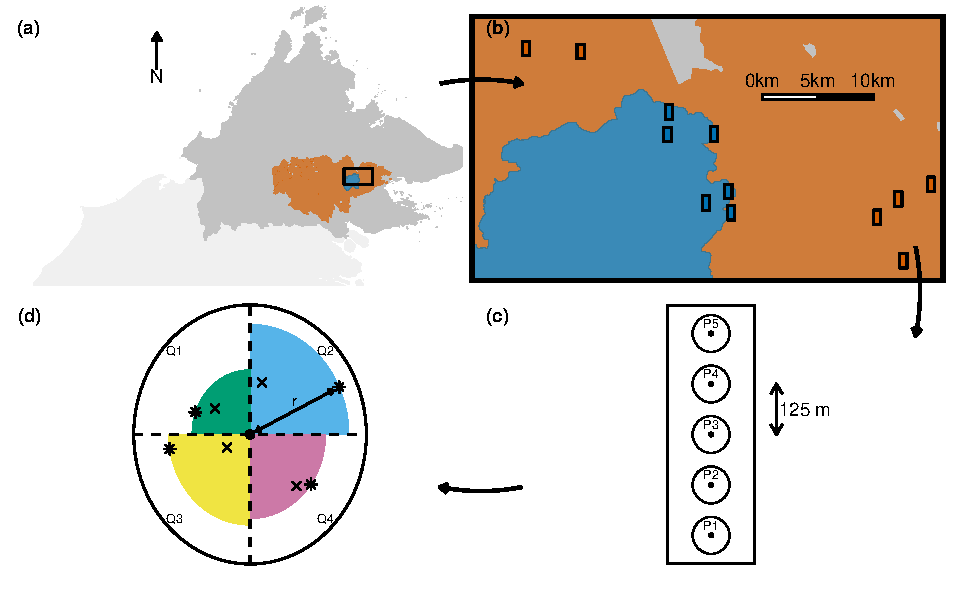
\includegraphics{./output/fig-4-1-1} 

}

\caption{Study location in Malaysian Borneo (a), and distribution of sites (b): six sites in primary forest (blue) and six sites in logged forest (orange). Each site comprised five plots along an existing transect, with plot centres separated by 125 m (c). Tree and sapling stand basal area was calculated from the distance to and circumference of the nearest two trees and saplings in each of four quadrants centred on the plot centre (d; see \autoref{text-B-1} for more details). Curved arrows indicate the direction of magnification, from panels a-d.}\label{fig:fig-4-1}
\end{figure}

\subsection{Sampling design}\label{sampling-design}

We sampled twelve sites, six in twice-logged forest and six in primary
forest, along existing transects
\citep[\autoref{fig:fig-4-1}b;][]{edwards_degraded_2011, edwards_selective-logging_2014}.
Sites were more than 2 km apart, and at least 100 m from forest edges.
Within each site, we established five plots 50 m in diameter, with plot
centres spaced at 125 m intervals along the transect
(\autoref{fig:fig-4-1}c; 60 plots in total). Fieldwork was conducted
from April to July 2015, during the severe El Niño-Southern Oscillation
(ENSO) event of 2015-2016 \citep{noaa_2015} when mean daily temperature
was 2.26°C higher and mean daily rainfall was 2.09 mm lower than the
5-year average (across April to July for the years 2007 to 2011; data
from weather station at Danum Valley Field Centre).

\subsubsection*{Forest structure}\label{forest-structure}
\addcontentsline{toc}{subsubsection}{Forest structure}

To quantify the level of disturbance to the forest from selective
logging, we used an established methodology for assessing forest
structure in each plot \citep{hamer_ecology_2003, lucey_spillover_2012}.
The variables we measured were: the stand basal area
(m\textsuperscript{2}/ha) of mature trees (circumference \textgreater{}
0.6 m) and saplings (circumference 0.1-0.6 m), based on the distance to
and circumference at breast height of the two nearest trees and saplings
in each of four quadrants centred on the plot centre
(\autoref{fig:fig-4-1}d); the coefficient of variation for the basal
area of trees and of saplings; the proportion of mature trees that were
dipterocarps (indicative of mature, complex forest); percentage canopy
cover; and visual estimates of percentage vegetation cover at ground
(1.5 m above ground), understorey (15 m above ground) and canopy (the
main stratum of leaf cover \textgreater{} 15 m above ground) height. For
full methodological details see \autoref{text-B-1}.

\subsubsection*{Quantifying surface
microclimates}\label{quantifying-surface-microclimates}
\addcontentsline{toc}{subsubsection}{Quantifying surface microclimates}

Fine-scale surface temperature of the forest floor is particularly
relevant for small-bodied, surface-dwelling organisms, such as many
insect and reptile species. We measured surface temperature within each
plot using an infrared camera (FLIR Systems, model E40). Macroclimate
temperature was defined as the air temperature at 1.5 m above-ground,
measured using a whirling hygrometer. Each site was visited on two days,
and each plot within the site was sampled five times each day between
05:00 hrs to 14:30 hrs. During each sample of any given plot, the
observer stood at the centre of the plot, took a single hygrometer
reading and then, holding the camera at breast height and pointing 45°
downwards (relative to the ground), took a photo in four orthogonal
directions \citep{scheffers_extreme_2017}. Each thermal image comprised
19200 distinct observations of surface temperature (one per pixel), and
covered a surface area of approximately 1 m\textsuperscript{2}. In
total, we recorded 2400 thermal images (4 images per plot x 5 repeats x
2 site visits x 60 plots).

For all subsequent analyses, a unique data point comprised thermal
information from the four photographs taken each time a plot was
sampled: 76800 observations of surface temperature measurements for each
plot (i.e.~combining 19200 observations from the four photos taken in
each orthogonal direction). For details of thermal image data extraction
and processing see \autoref{text-B-2}. The temperature of cool surface
microclimates was defined as the 5\textsuperscript{th} percentile
(i.e.~coolest) across all 76800 pixels. For some organisms, the efficacy
of thermal buffering also depends on the thermal stability of
microclimates \citep{shi_framework_2016}. We calculated daily variation
in surface microclimate temperature as the difference between the
minimum and maximum microclimate temperature, for each day and for each
plot.

To identify spatially-explicit patches of warm and cool pixels
(\autoref{fig:fig-4-2}) we calculated the Getis-Ord local statistic for
each pixel within the neighbourhood of the nearest eight pixels, using
the function `localG' in the spdep package in R
\citep{bivand_comparing_2015, r_core_team_2017}. Pixels with a Z-value
of ≥ 3.886 were defined as being within warm patches, and those with a
Z-value of ≤ -3.886 within cool patches \citep{getis_local_1996}.
Thermal diversity was defined as the difference between the median
temperature of the warmest warm patch minus the median temperature of
the coolest cool patch (hereafter: `patch temperature range'). The
average surface area of cool patches was calculated as the total number
of pixels within cool patches, multiplied by the surface area of one
pixel (0.516 cm\textsuperscript{2}), and divided by the total number of
cool patches across the four photos. Finally, spatial configuration of
cool patches was quantified using the Aggregation Index: the number of
edges that cool patches share, divided by the maximum number of edges
that they could possibly share
\citep{he_aggregation_2000, caillon_warming_2014}. Higher values of the
Aggregation Index indicate increased clustering of microclimates in
space, which makes them more difficult for organisms to track
\citep{sears_configuration_2016}.

\begin{figure}

{\centering 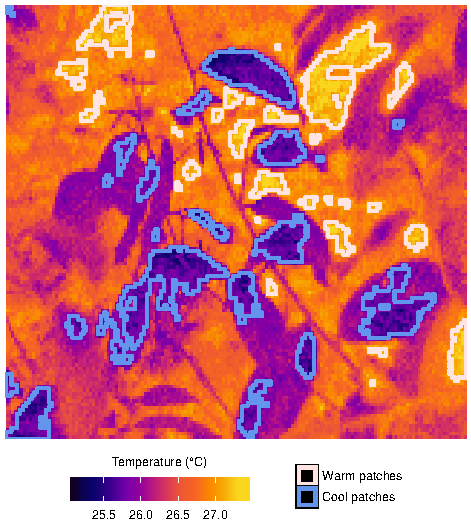
\includegraphics{./output/fig-4-2-1} 

}

\caption{Example thermal image. Pixels are shaded from cold (purple) to hot (yellow). Warm patches (outlined in pink) and cool patches (outlined in blue) were identified using the Getis-Ord local statistic of each pixel.}\label{fig:fig-4-2}
\end{figure}

\subsubsection*{Quantifying microclimates in leaf litter, tree holes and
deadwood}\label{quantifying-microclimates-in-leaf-litter-tree-holes-and-deadwood}
\addcontentsline{toc}{subsubsection}{Quantifying microclimates in leaf
litter, tree holes and deadwood}

Many ectotherms, such as amphibians, spend some or all of their time
exploiting cool microclimates inside microhabitats, which thermal images
are unable to capture. We selected three types of microhabitat known to
provide cool microclimates
\citep{scheffers_microhabitats_2014, scheffers_microhabitats_2014-1, gonzalez_del_pliego_thermally_2016},
and placed one temperature datalogger (HOBO pendant datalogger, Onset,
model UA-001-64K or model UA-002-64K) per plot in each microhabitat
type: deadwood (\textgreater{} 10 cm stem diameter), tree holes
(\textgreater{} 2 cm at widest point of entrance hole, \textless{} 2 m
above the ground) and leaf litter (1.5 m left of the plot centre). The
hygrometer measurements of macroclimate temperature were not always
synchronised with the dataloggers inside microhabitats, hence we
additionally measured macroclimate temperature using a datalogger
suspended 1.5 m above the ground at the centre of each plot, shielded
against direct radiation and precipitation by an inverted plastic funnel
\citep{shoo_potential_2010, scheffers_microhabitats_2014-1}.

All dataloggers recorded temperature every 20 minutes for six
consecutive days, occurring within one week of thermal image collection.
For qualitative comparison with thermal images and to lessen the degree
of temporal autocorrelation, microclimate temperatures for each of the
three microhabitats in each plot were calculated as the median of six
daily measures, computed for each two-hour interval during the same time
period as when thermal images were collected (i.e.~04:40 to 14:40 hrs).
Our analyses focused on day-time thermal buffering, but we also ran
analogous models for the full 24 hours to explore night-time thermal
buffering (see \autoref{text-B-5}). In the main text, we only present
data for day-time measurements because this is most relevant to
organisms seeking to avoid extremes of heat, and because findings were
qualitatively similar. Variation in temperature for microclimates inside
microhabitats was defined as the daily range (95\textsuperscript{th}
percentile minus 5\textsuperscript{th} percentile) of raw temperatures
for each day, in each plot.

To estimate the occurrence of microclimates inside microhabitats, we
measured the volume of leaf litter, tree holes and deadwood within a 50
x 5 m subplot centred on each plot centre (60 sub-plots in total), with
the long edge running parallel to the transect. For full methodological
details see \autoref{text-B-3}. We divided microhabitat volume by the
total area surveyed to generate microhabitat volume per
m\textsuperscript{2} forest, for each plot.

\subsection{Variables analysed}\label{variables-analysed}

\subsubsection*{Forest structure}\label{forest-structure-1}
\addcontentsline{toc}{subsubsection}{Forest structure}

We examined the impact of selective logging on forest structure using
linear mixed effects models to compare nine structural response
variables between logged and primary forests: stand basal area of trees
and of saplings; the coefficient of variation across individual basal
areas of trees and of saplings; proportion of trees that were
dipterocarps (binomial data: dipterocarp versus non-dipterocarp);
percentage canopy cover (proportion data); and percentage vegetation
cover at ground, understorey and canopy strata (proportion data). We
found that tree stand basal area (m\textsuperscript{2}/ha) was a good
measure of changes in forest structure from logging activity (LR =
8.102, \emph{P} \textless{} 0.01; \autoref{fig:fig-B-2}a; see Results
for full details), hence we use this variable as a continuous measure of
disturbance (henceforth: forest quality) in all our analyses exploring
the thermal buffering potential of logged and unlogged forests.

\subsubsection*{Macroclimate and microclimate
temperature}\label{macroclimate-and-microclimate-temperature}
\addcontentsline{toc}{subsubsection}{Macroclimate and microclimate
temperature}

Macroclimate temperature is the temperature at a relatively coarse
spatial scale, and was captured in this study using both a hygrometer
and suspended datalogger (measuring the same variable but at different
times). The macroclimate does not affect thermal buffering potential
\emph{per se}, but it does dictate the overall necessity for thermal
buffering. We modelled hygrometer and datalogger temperature separately,
including forest type (logged or primary forest) and forest quality as
explanatory variables (see \autoref{text-B-4}).

To assess the impact of selective logging on the ability of
microclimates to buffer organisms from macroclimate warming, we modelled
microclimate temperature against forest quality, forest type and
macroclimate temperature, including an interaction term between the
latter two variables. The slope of the relationship between microclimate
and macroclimate temperature is a measure of the rate of change. Surface
microclimate temperature refers to the 5\textsuperscript{th} percentile
of surface temperature observations (i.e.~coolest) for each plot, and
this was compared against macroclimate temperature as measured by the
hygrometer. Microclimate temperature inside leaf litter, tree holes and
deadwood refers to the two-hourly median temperature recorded by
dataloggers inside microhabitats, and this was compared against
macroclimate temperature as measured by a suspended datalogger.

To capture the impact of logging on the thermal stability of
microclimates, we modelled microclimate temperature range against forest
type and forest quality. For surface microclimates, the range was the
daily range of surface temperature observations (the
5\textsuperscript{th} percentiles, i.e.~coolest surface temperatures).
For microclimates inside microhabitats, the range was the daily range
(95\textsuperscript{th} percentile minus 5\textsuperscript{th}
percentile) of the raw temperature observations. All models were run
separately for surface, leaf litter, tree hole and deadwood
microclimates.

\subsubsection*{Microclimate
availability}\label{microclimate-availability}
\addcontentsline{toc}{subsubsection}{Microclimate availability}

Microclimate occurrence was modelled separately for surface
microclimates (i.e.~the average surface area of cool patches), and those
inside leaf litter, tree holes and deadwood (each quantified by their
average volume per m\textsuperscript{2} forest). The thermal diversity
of surface microclimates was captured by the temperature range between
the warmest warm patch and the coolest cool patch. The spatial
configuration of surface microclimates refers to the Aggregation Index
of cool patches (binomial data: edges shared by cool patches versus
edges not shared by cool patches). For all models, the fixed effects
were forest type (logged or primary forest) and forest quality
(i.e.~tree stand basal area).

\subsection{Statistical analyses}\label{statistical-analyses}

All data were analysed using mixed effects models in R \citep[version
3.3.0;][]{r_core_team_2017}. To account for spatial pseudoreplication,
forest structure models included `site' as a random intercept term, and
all other models included `plot' nested within `site'. Temperature data
were recorded at multiple time points, hence the full models were
visually assessed for evidence of temporal autocorrelation of residuals
\citep[function `acf' in the nlme package;][]{pinheiro_nlme:_2017}, and
a correlation structure for both date and time was incorporated where
necessary \citep[the specific structure was chosen using
AIC;][]{zuur_mixed_2009}. For binomial data (proportion of dipterocarps
and surface microclimate Aggregation Index) we used generalized linear
mixed effects models (GLMMs) with a binomial error distribution, fitted
using the package lme4 \citep{bates_fitting_2015} and tested for
overdispersion. Diagnostic plots were assessed for all models to confirm
model fit and, where necessary, we modified the variance structure of
the residuals \citep{zuur_mixed_2009} and transformed variables to
normality. For true proportion data (percentage canopy cover and
percentage vegetation cover), the transformation used was a modification
of the empirical logit \citep{warton_arcsine_2011}.

For all models, statistical significance was inspected using likelihood
ratio tests, dropping each fixed effect in turn and comparing it to the
full model \citep{zuur_mixed_2009}. The significance of main effects
involved in an interaction was assessed in the same way, except reduced
models were compared to a full model without the interaction term. The
basic structure for most response variables (RV) was:

\texttt{RV\ \textasciitilde{}\ forest\_type\ +\ forest\_quality\ +\ (1\textbar{}transect/plot)\ +\ cor(\textasciitilde{}\ date\_time\textbar{}transect/plot)}

\section{Results}\label{results-2}

\subsection{Changes in forest structure after
logging}\label{changes-in-forest-structure-after-logging}

Following two rounds of commercial selective logging, tree stand basal
area -- our measure of forest quality -- was 39.5
m\textsuperscript{2}/ha in logged forest, compared to 39.5
m\textsuperscript{2}/ha in primary forest (LR = 8.102, \emph{P}
\textless{} 0.01; \autoref{fig:fig-B-2}a). Logged forests thus contained
far fewer large trees than did primary forests. There were also more
large saplings in logged forest (6.77 m\textsuperscript{2}/ha) than in
primary forests (6.77 m\textsuperscript{2}/ha; LR = 4.239, \emph{P}
\textless{} 0.05; \autoref{fig:fig-B-2}b), and trees were less variable
in size (LR = 13.038, \emph{P} \textless{} 0.001;
\autoref{fig:fig-B-2}c). There was no difference between forest types in
terms of the variability of size among saplings (LR = 0.114, \emph{P} =
0.736; \autoref{fig:fig-B-2}d).

Changes to forest structure from selective logging were also evident in
the overall amount of vegetation cover. Although there was no observed
difference between logged forest and primary forest in percentage
vegetation at ground level (LR = 2.758, \emph{P} = 0.097;
\autoref{fig:fig-B-2}g), the proportion of trees that were dipterocarps
(Χ² = 2.42, \emph{P} = 0.12; \autoref{fig:fig-B-2}e) or the percentage
canopy cover (LR = 0.874, \emph{P} = 0.35; \autoref{fig:fig-B-2}f), we
did find that percentage vegetation cover was higher in primary forest
than in logged forest in both the understorey (primary = 68.2\%; logged
= 68.2\%; LR = 5.288, \emph{P} \textless{} 0.05;
\autoref{fig:fig-B-2}h), and in the canopy (primary = 23.1\%; logged =
23.1\%; LR = 9.174, \emph{P} \textless{} 0.01; \autoref{fig:fig-B-2}i).
Thus, 9-12 years after logging there were significant differences in
forest structure between logged and primary forests. This was especially
true for the components of forest structure that typically indicate the
presence of large, mature trees and high structural complexity, and
which might be expected to influence microclimates and the availability
of microhabitats.

\subsection{Macroclimate and microclimate temperature in logged and
primary
forest}\label{macroclimate-and-microclimate-temperature-in-logged-and-primary-forest}

Despite differences in forest structure, we found no difference in
macroclimate temperature of logged and primary forests, whether measured
by the hygrometer (LR = 0.081, \emph{P} = 0.776; \autoref{fig:fig-B-3}a)
or suspended datalogger (LR = 0, \emph{P} = 0.983;
\autoref{fig:fig-B-3}b). Macroclimate temperature was also consistent
across varying levels of forest quality, for temperature measured via
the hygrometer (LR = 0.022, \emph{P} = 0.883; \autoref{fig:fig-B-3}a)
and suspended datalogger (LR = 0.527, \emph{P} = 0.468;
\autoref{fig:fig-B-3}b). Thus, the necessity for thermal buffering was
comparable between the two forest types.

Absolute microclimate temperature was comparable between forest types
for all of the microclimates considered: surface (LR = 0.447, \emph{P} =
0.504; \autoref{fig:fig-4-3}e), deadwood (LR = 0.206, \emph{P} = 0.65;
\autoref{fig:fig-4-3}f), tree holes (LR = 2.759, \emph{P} = 0.097;
\autoref{fig:fig-4-3}g) and leaf litter (LR = 1.616, \emph{P} = 0.204;
\autoref{fig:fig-4-3}h). We found that the relationship between
microclimate temperature and macroclimate temperature was slightly
steeper in primary forest compared to logged forest for deadwood (LR =
7.268, \emph{P} \textless{} 0.01; \autoref{fig:fig-4-3}b), tree holes
(LR = 13.657, \emph{P} \textless{} 0.001; \autoref{fig:fig-4-3}c) and
leaf litter (LR = 28.914, \emph{P} \textless{} 0.001;
\autoref{fig:fig-4-3}d). However, for 1°C macroclimate warming (from the
median value) the maximum difference in microclimate warming between
forest types was \textless{} 0.1°C, and no such interaction was apparent
for surface microclimates (LR = 1.197, \emph{P} = 0.274;
\autoref{fig:fig-4-3}a). Similarly, for a 1 m\textsuperscript{2}/ha
increase in forest quality (i.e.~tree stand basal area), tree hole
temperature was slightly warmer (LR = 4.661, \emph{P} \textless{} 0.05;
\autoref{fig:fig-4-3}g), but the size of this effect was negligible
(+0.00194°C), and not evident for other microclimates (\emph{P}
\textgreater{} 0.05; \autoref{fig:fig-4-3}e-h). Thus we conclude that
effects of logging on microclimate temperature were generally not
evident, or minimal.

The final facet of microclimate temperature that we considered was daily
temperature variation. This too was comparable between logged and
primary forests for microclimates at the surface (LR = 0.437, \emph{P} =
0.508; \autoref{fig:fig-4-4}a), as well as those inside deadwood (LR =
0.02, \emph{P} = 0.889; \autoref{fig:fig-4-4}b), tree holes (LR = 3.242,
\emph{P} = 0.072; \autoref{fig:fig-4-4}c) and leaf litter (LR = 2.449,
\emph{P} = 0.118; \autoref{fig:fig-4-4}d). Microclimate temperature
variation was also consistent across different levels of forest quality
(\emph{P} \textgreater{} 0.05; \autoref{fig:fig-4-4}).

In summary, selective logging had little observed impact on absolute
microclimate temperature or its daily variation. There was some evidence
that thermal buffering potential was slightly enhanced for deadwood,
tree holes and leaf litter inside logged forest, but the effects were
extremely small and not evident for microclimates at the surface.

\begin{figure}

{\centering 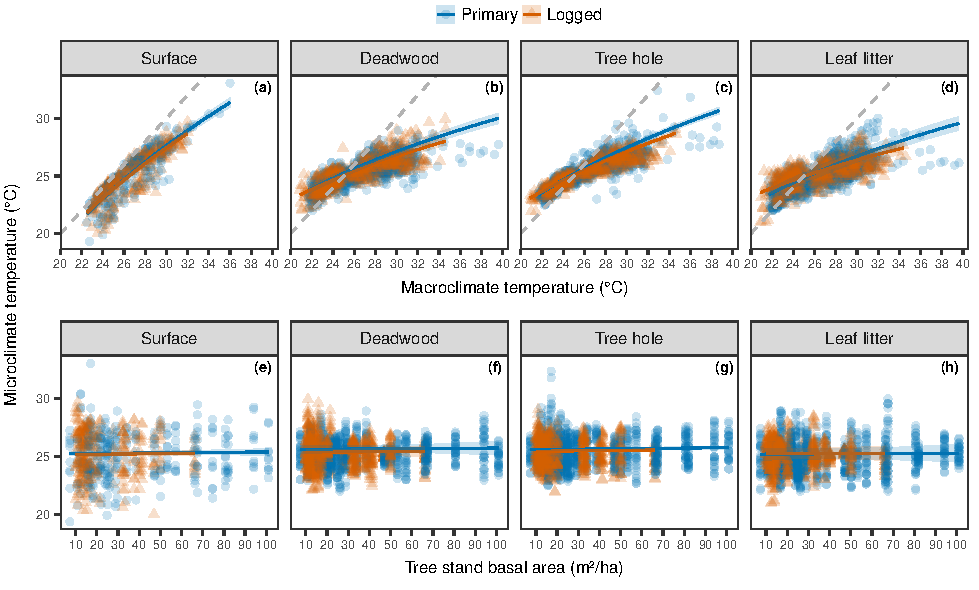
\includegraphics{./output/fig-4-3-1} 

}

\caption{Comparison between primary forest (blue) and logged forest (orange) in terms of: (a-d) the relationship between microclimate temperature and macroclimate temperature; and (e-h) absolute microclimate temperature across varying levels of forest quality (measured as tree stand basal area). Microclimates were measured at the surface (a, e), and inside deadwood (b, f), tree holes (c, g)  and leaf litter (d, h). The grey dashed lines in panels a-d indicate zero temperature buffering, where the microclimate temperature is equal to the macroclimate temperature. In all panels, shaded bands are 95\% confidence intervals.}\label{fig:fig-4-3}
\end{figure}














\begin{figure}

{\centering 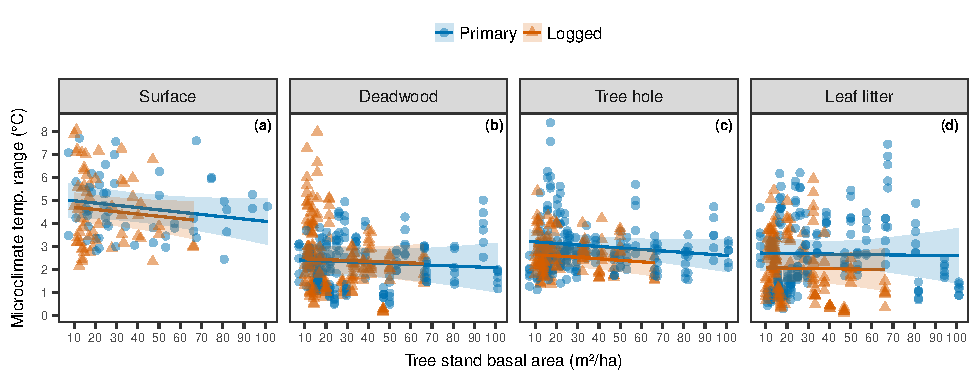
\includegraphics{./output/fig-4-4-1} 

}

\caption{The influence of forest type (primary or logged) and
forest quality (measured as tree stand basal area) on microclimate
temperature range. Daily range for surface microclimates (a) was
calculated as the difference between the maximum and the minimum
microclimate temperature (itself calculated as the 5\textsuperscript{th}
percentile temperature across four photos taken at each visit to each
plot). For microclimates inside deadwood (b), tree holes (c) and leaf
litter (d), the daily range was the difference between the
95\textsuperscript{th} percentile and 5\textsuperscript{th} percentile
of raw temperature measurements. Primary forest data points are depicted
as blue circles and logged forest as orange triangles. Shaded bands
represent 95\% confidence intervals.}\label{fig:fig-4-4}
\end{figure}

\subsection{Microclimate availability in logged and primary
forest}\label{microclimate-availability-in-logged-and-primary-forest}

The thermal buffering potential within a habitat depends not only on the
temperature of microclimates relative to the macroclimate, but also on
the overall availability and thermal diversity of those microclimates.
The occurrence of surface microclimates was not impacted by forest type
(LR = 0.872, \emph{P} = 0.35; \autoref{fig:fig-4-5}b), and the average
volume of microhabitats (per m\textsuperscript{2} forest) was similar in
logged and primary forest for deadwood (LR = 0.263, \emph{P} = 0.608;
\autoref{fig:fig-4-5}d), tree holes (LR = 3.053, \emph{P} = 0.081;
\autoref{fig:fig-4-5}e) and leaf litter (LR = 0.162, \emph{P} = 0.687;
\autoref{fig:fig-4-5}f). There was no observed impact of forest quality
on the occurrence of surface microclimates (LR = 1.324, \emph{P} = 0.25;
\autoref{fig:fig-4-5}b) or the volume of deadwood (LR = 3.78, \emph{P} =
0.052; \autoref{fig:fig-4-5}d) and tree holes (LR = 2.172, \emph{P} =
0.141; \autoref{fig:fig-4-5}e). In contrast, we found that leaf litter
volume increased by 12.3 cm\textsuperscript{3}/m\textsuperscript{2} for
a 1 m\textsuperscript{2}/ha increase in forest quality (i.e.~tree stand
basal area; LR = 7.056, \emph{P} \textless{} 0.01;
\autoref{fig:fig-4-5}f).

Using thermal images we were able to quantify the thermal diversity and
spatial configuration of surface microclimates. Thermal diversity has a
bearing on the diversity of organisms that are able to find
microclimates meeting their thermal requirements (which vary according
to species, age, time of day, seasonality, etc.). Spatial configuration
influences the ease with which organisms can utilise microclimates. We
found that the temperature range spanned by surface microclimates (both
warm and cool patches) was comparable between logged and primary forests
(LR = 0.276, \emph{P} = 0.599; \autoref{fig:fig-4-5}a) and with varying
forest quality (LR = 3.552, \emph{P} = 0.059; \autoref{fig:fig-4-5}a).
The same was true for the Aggregation Index of cool surface patches,
both between logged and primary forest (Χ² = 0.312, \emph{P} = 0.576;
\autoref{fig:fig-4-5}c) and with different levels of forest quality (Χ²
= 0.183, \emph{P} = 0.669; \autoref{fig:fig-4-5}c).

Overall, the availability of microclimates was minimally affected by
selective logging, regardless of whether microclimates were located at
the surface or inside microhabitats. This was true for various different
components of microclimate availability, including their occurrence,
thermal diversity and spatial configuration.

\begin{figure}

{\centering 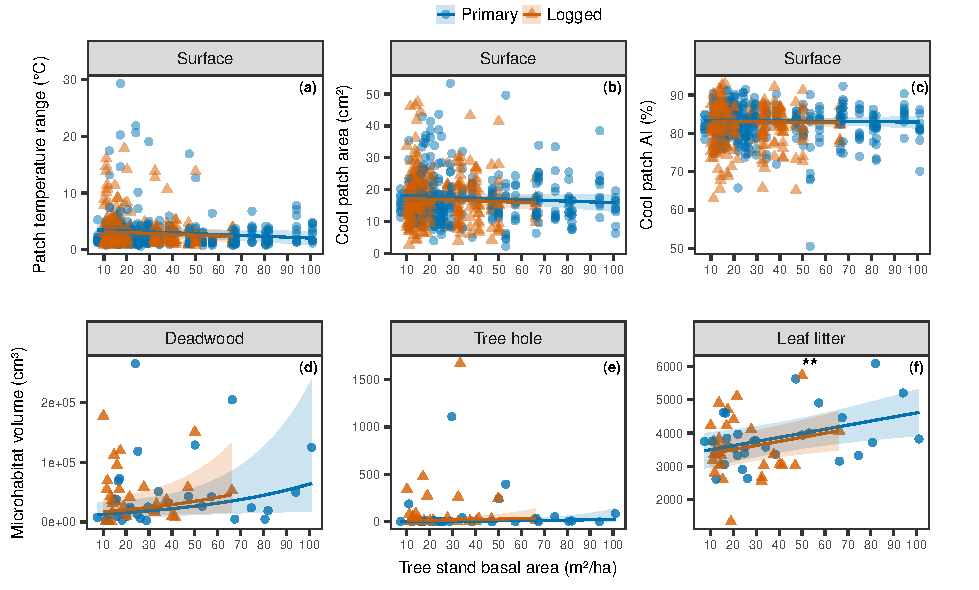
\includegraphics{./output/fig-4-5-1} 

}

\caption{The influence of forest type (primary or logged forest)
and forest quality (measured as tree stand basal area) on microclimate
availability. Results for surface microclimates (top row) include: the
temperature range from the warmest warm patch to the coolest cool patch
(a); the average surface area of cool patches (b); and the Aggregation
Index of cool patches (c). The volume (per m\textsuperscript{2} forest)
of microhabitats typically associated with microclimates (bottom row) is
shown for deadwood (d), tree holes (e) and leaf litter (f). Primary
forest data points are depicted as blue circles and logged forest as
orange triangles. Shaded bands represent 95\% confidence intervals.
Asterisks in panel f denote a statistically significant difference at
0.001 \textless{} \emph{P} \textless{} 0.01 (**).}\label{fig:fig-4-5}
\end{figure}














\section{Discussion}\label{discussion-2}

Forest degradation by commercial selective logging affects huge expanses
of the tropics \citep{asner_contemporary_2009, lewis_increasing_2015}.
Southeast Asia has experienced the most intensive selective logging of
all tropical rainforests \citep{lewis_increasing_2015}, and in our study
area \textasciitilde{}145 m\textsuperscript{3} of timber was removed per
hectare. Despite these forests having only a maximum of 12 years
post-logging recovery \citep{fisher_cost-effective_2011}, and the
coincidental occurrence during data collection of abnormally hot and dry
conditions associated with the strongest El Niño-Southern Oscillation
(ENSO) event since 1998 \citep{noaa_2015}, we found very few thermal
differences associated with selective logging. This is an important
finding for tropical conservation because it suggests that the potential
for thermal buffering will not limit the ability of selectively logged
forests to maintain high biodiversity under climate change.

\subsection{Forest structure}\label{forest-structure-2}

At a local scale (m to ha), climate is highly dependent upon vegetation
\citep{oke_boundary_1987, sears_world_2011}. Selective logging
operations generally target larger and older trees, leading to many
associated changes in vegetation structure
\citep{okuda_effect_2003, kumar_effects_2005, edwards_maintaining_2014}.
A clear signal of historical logging in our study area was a reduction
in stand basal area of mature trees by 0\%
\citep[\autoref{fig:fig-B-2}a;][]{berry_impacts_2008}, accompanied by
reduced variation in tree basal area (\autoref{fig:fig-B-2}c), and
reduced vegetation cover at ≥ 15 m height (\autoref{fig:fig-B-2}h,i).
The increase in stand basal area of saplings by 0\%
(\autoref{fig:fig-B-2}b) is evidence that there has been substantial
natural regeneration in the intervening years.

\subsection{Macroclimate and microclimate
temperature}\label{macroclimate-and-microclimate-temperature-1}

Although primary forest contained more large trees
(\autoref{fig:fig-B-2}a), the absence of any long-term effect of
selective logging on percentage canopy cover (\autoref{fig:fig-B-2}f)
suggests that forest vegetation as a whole -- regardless of how it was
distributed vertically -- intercepted comparable amounts of incoming
solar radiation in both logged and primary forests. This finding is in
keeping with previous studies observing rapid horizontal canopy growth
following selective logging \citep[e.g.][]{asner_canopy_2004}.
Alternatively, vegetation in logged forest may have intercepted less
incoming radiation than in primary forest (i.e.~if there was less
vegetation overall), but reflected a greater proportion of what was
intercepted, owing to the higher albedo of habitats with an abundance of
non-tree species
\citep{oke_boundary_1987, davin_climatic_2010, edwards_maintaining_2014}.
In either case (or in combination), given comparable levels of solar
radiation reaching the forest floor of logged and primary forests, it
follows that the temperature at coarse and fine scales (macroclimate and
microclimate temperatures) should also be comparable
(\autoref{fig:fig-4-3} and \autoref{fig:fig-B-3}).

The temperature of cool microclimates relative to average conditions is
what largely determines their ability to buffer macroclimate warming
\citep{scheffers_microhabitats_2014-1, gonzalez_del_pliego_thermally_2016, shi_framework_2016}.
Given that selective logging did not affect absolute temperature of the
macroclimate (\autoref{fig:fig-B-3}) or microclimates
(\autoref{fig:fig-4-3}), we can infer that there was no overall effect
of selective logging on the difference between micro- and macroclimate
temperature. There was also no evidence that selective logging impacted
overall daily variation in microclimate temperature
(\autoref{fig:fig-4-4}). There were some impacts of logging on the
relationship between microclimate and macroclimate temperature for
microclimates inside deadwood, tree holes and leaf litter
(\autoref{fig:fig-4-3}), but the effect sizes for these interactions
were extremely small. The maximum difference in microclimate warming
between logged and primary forests was \textless{} 0.1°C for 1°C of
macroclimate warming. As such, we conclude that even when selective
logging had a statistically significant influence on thermal buffering
potential, the effect was small and of limited biological relevance.

\subsection{Microclimate
availability}\label{microclimate-availability-1}

Even if microclimates are present and effective at buffering temperature
change, overall rarity or isolation could render them functionally
redundant to some species
\citep{sears_world_2011, sears_configuration_2016}. We demonstrate that
lower forest quality was associated with less leaf litter
\citep[\autoref{fig:fig-4-5}; cf.][]{saner_reduced_2009}, but forest
quality and forest type had little effect on the occurrence of
microclimates at the surface or inside deadwood and tree holes. This is
contrary to expectations from previous studies
\citep{ball_tree_1999, blakely_tree_2008}. However, high volumes of
deadwood could be maintained in logged forest by lower decomposition
rates
\citetext{\citealp{ewers_logging_2015}; \citealp{yeong_leaf_2016}; \citealp[but
see][]{herault_modeling_2010}}, and large remnant pieces from harvest
operations. In undisturbed forests, tree holes tend to be associated
with larger, older trees
\citep{lindenmayer_cavity_2000, blakely_tree_2008}. A comparable
quantity of tree holes might be found in logged forests because of
damage from logging operations \citep{edwards_maintaining_2014},
increased wind in gaps \citep{chen_growing-season_1995} and remnant
large trees that were specifically avoided by logging companies because
of hollow boles. Additionally, we assessed tree holes in the understorey
only, and differences may well manifest at higher forest strata.

The availability of microclimates to organisms is also influenced by
their thermal diversity and distribution in space. We found that patches
of warm and cool microclimates on the surface of the forest floor
spanned a temperature range of about 3°C, regardless of logging activity
(\autoref{fig:fig-4-5}a). Cool patches were generally highly clustered
in space (Aggregation Index of 83.3\%), but this was not affected by
logging (\autoref{fig:fig-4-5}c). Thermal diversity and spatial
configuration of microclimates are relatively novel facets of thermal
buffering potential \citep[but
see:][]{caillon_warming_2014, sears_configuration_2016, faye_toolbox_2016};
they are likely determined by the composition of the forest floor and
the relative radiative properties of these different components
\citep[e.g.~bare soil versus leaves versus
water;][]{oke_boundary_1987, snyder_analyzing_2004}. We therefore
suggest that these characteristics of the forest floor were comparable
between forests despite the large differences in forest structure that
were evident after logging.

\subsection{Caveats and future research
directions}\label{caveats-and-future-research-directions}

The potential for thermal buffering and its general necessity are
influenced by moisture levels, as well as temperature
\citep{mclaughlin_hydrologic_2017}. Many ectotherms, including
amphibians \citep{duellman_biology_1986} and isopods
\citep{hassall_predicting_2010}, can survive in hot temperatures for
longer if relative humidity is sufficiently high to prevent desiccation.
Although we did not measure fine-scale vapour pressure deficit (a
variable combining both temperature and relative humidity), we did find
that coarse-scale vapour pressure deficit measurements from the
hygrometer and from hygrochron iButtons (\autoref{text-B-4}) showed
little variation within or between forests (\autoref{fig:fig-B-3}).

Relative climates in primary and logged forests could be very different
above the understorey, which we were unable to capture in our study.
Some ectotherms move down from the upper strata to exploit more
favourable temperatures lower down \citep{scheffers_increasing_2013}.
Hence, if temperatures in higher strata are in fact hotter in logged
forest compared to primary forest, it is possible that species could
move to utilise the favourable temperatures of the understorey of logged
forest that we demonstrate here, potentially resulting in a `flattening'
of species' vertical distributions.

While thermal cameras are an important addition to the toolbox of
microclimate research \citep{faye_toolbox_2016}, it is also important to
remember that they are just one element. Thermal cameras are well-suited
to capturing temperature at a very fine-scale and with inherent spatial
information, but differences in 3D topography of a surface could affect
results (e.g.~the real distance between neighbouring pixels can be more
than is apparent in the 2D image). Additionally, although thermal
cameras are ideal for measuring surface temperatures, they have a
limited capacity to capture sub-surface temperatures, and hence we have
used thermal imagery in combination with dataloggers.

The ability of selectively logged tropical forests to retain current
levels of biodiversity will critically depend on their ability to
protect species from the impacts of increasingly severe climate change.
As average temperatures increase over this century, so too will the
intensity and frequency of extreme climatic events. Thermal buffering
will likely be crucial in allowing species to move locally to avoid
suboptimal climates. We sampled in some of the most intensively logged
forest in the tropics, during abnormally hot and dry conditions of a
severe ENSO event; it is highly unlikely that our study would have
failed to detect any appreciable thermal differences between primary and
logged forests had they existed. Regardless of whether commercially
selectively logged forests remain biologically or structurally
distinctive from undisturbed forests, this study shows for the first
time that they are functionally equivalent in the provisioning of cool
microclimates, and underscores their vital role in conservation both now
and under future climate warming.

\section{Data availability}\label{data-availability}

Data available from the University of Sheffield Online Research Data
repository (\url{https://doi.org/10.15131/shef.data.5414629}).

\section{Acknowledgements}\label{acknowledgements-2}

Thanks to staff at Danum Valley Field Centre for logistical support; and
Azlin Bin Sailim, Jessica Olid and Chloe Walker-Trivett for field
assistance. R.A.S. was funded by a NERC studentship through the ACCE
(Adapting to the Challenges of a Changing Environment) Doctoral Training
Partnership (Grant No. NE/L002450/1).

\chapter{The impact of recent forest cover change on climate
connectivity in the
tropics}\label{the-impact-of-recent-forest-cover-change-on-climate-connectivity-in-the-tropics}

\begin{figure}[!htb]
\centering
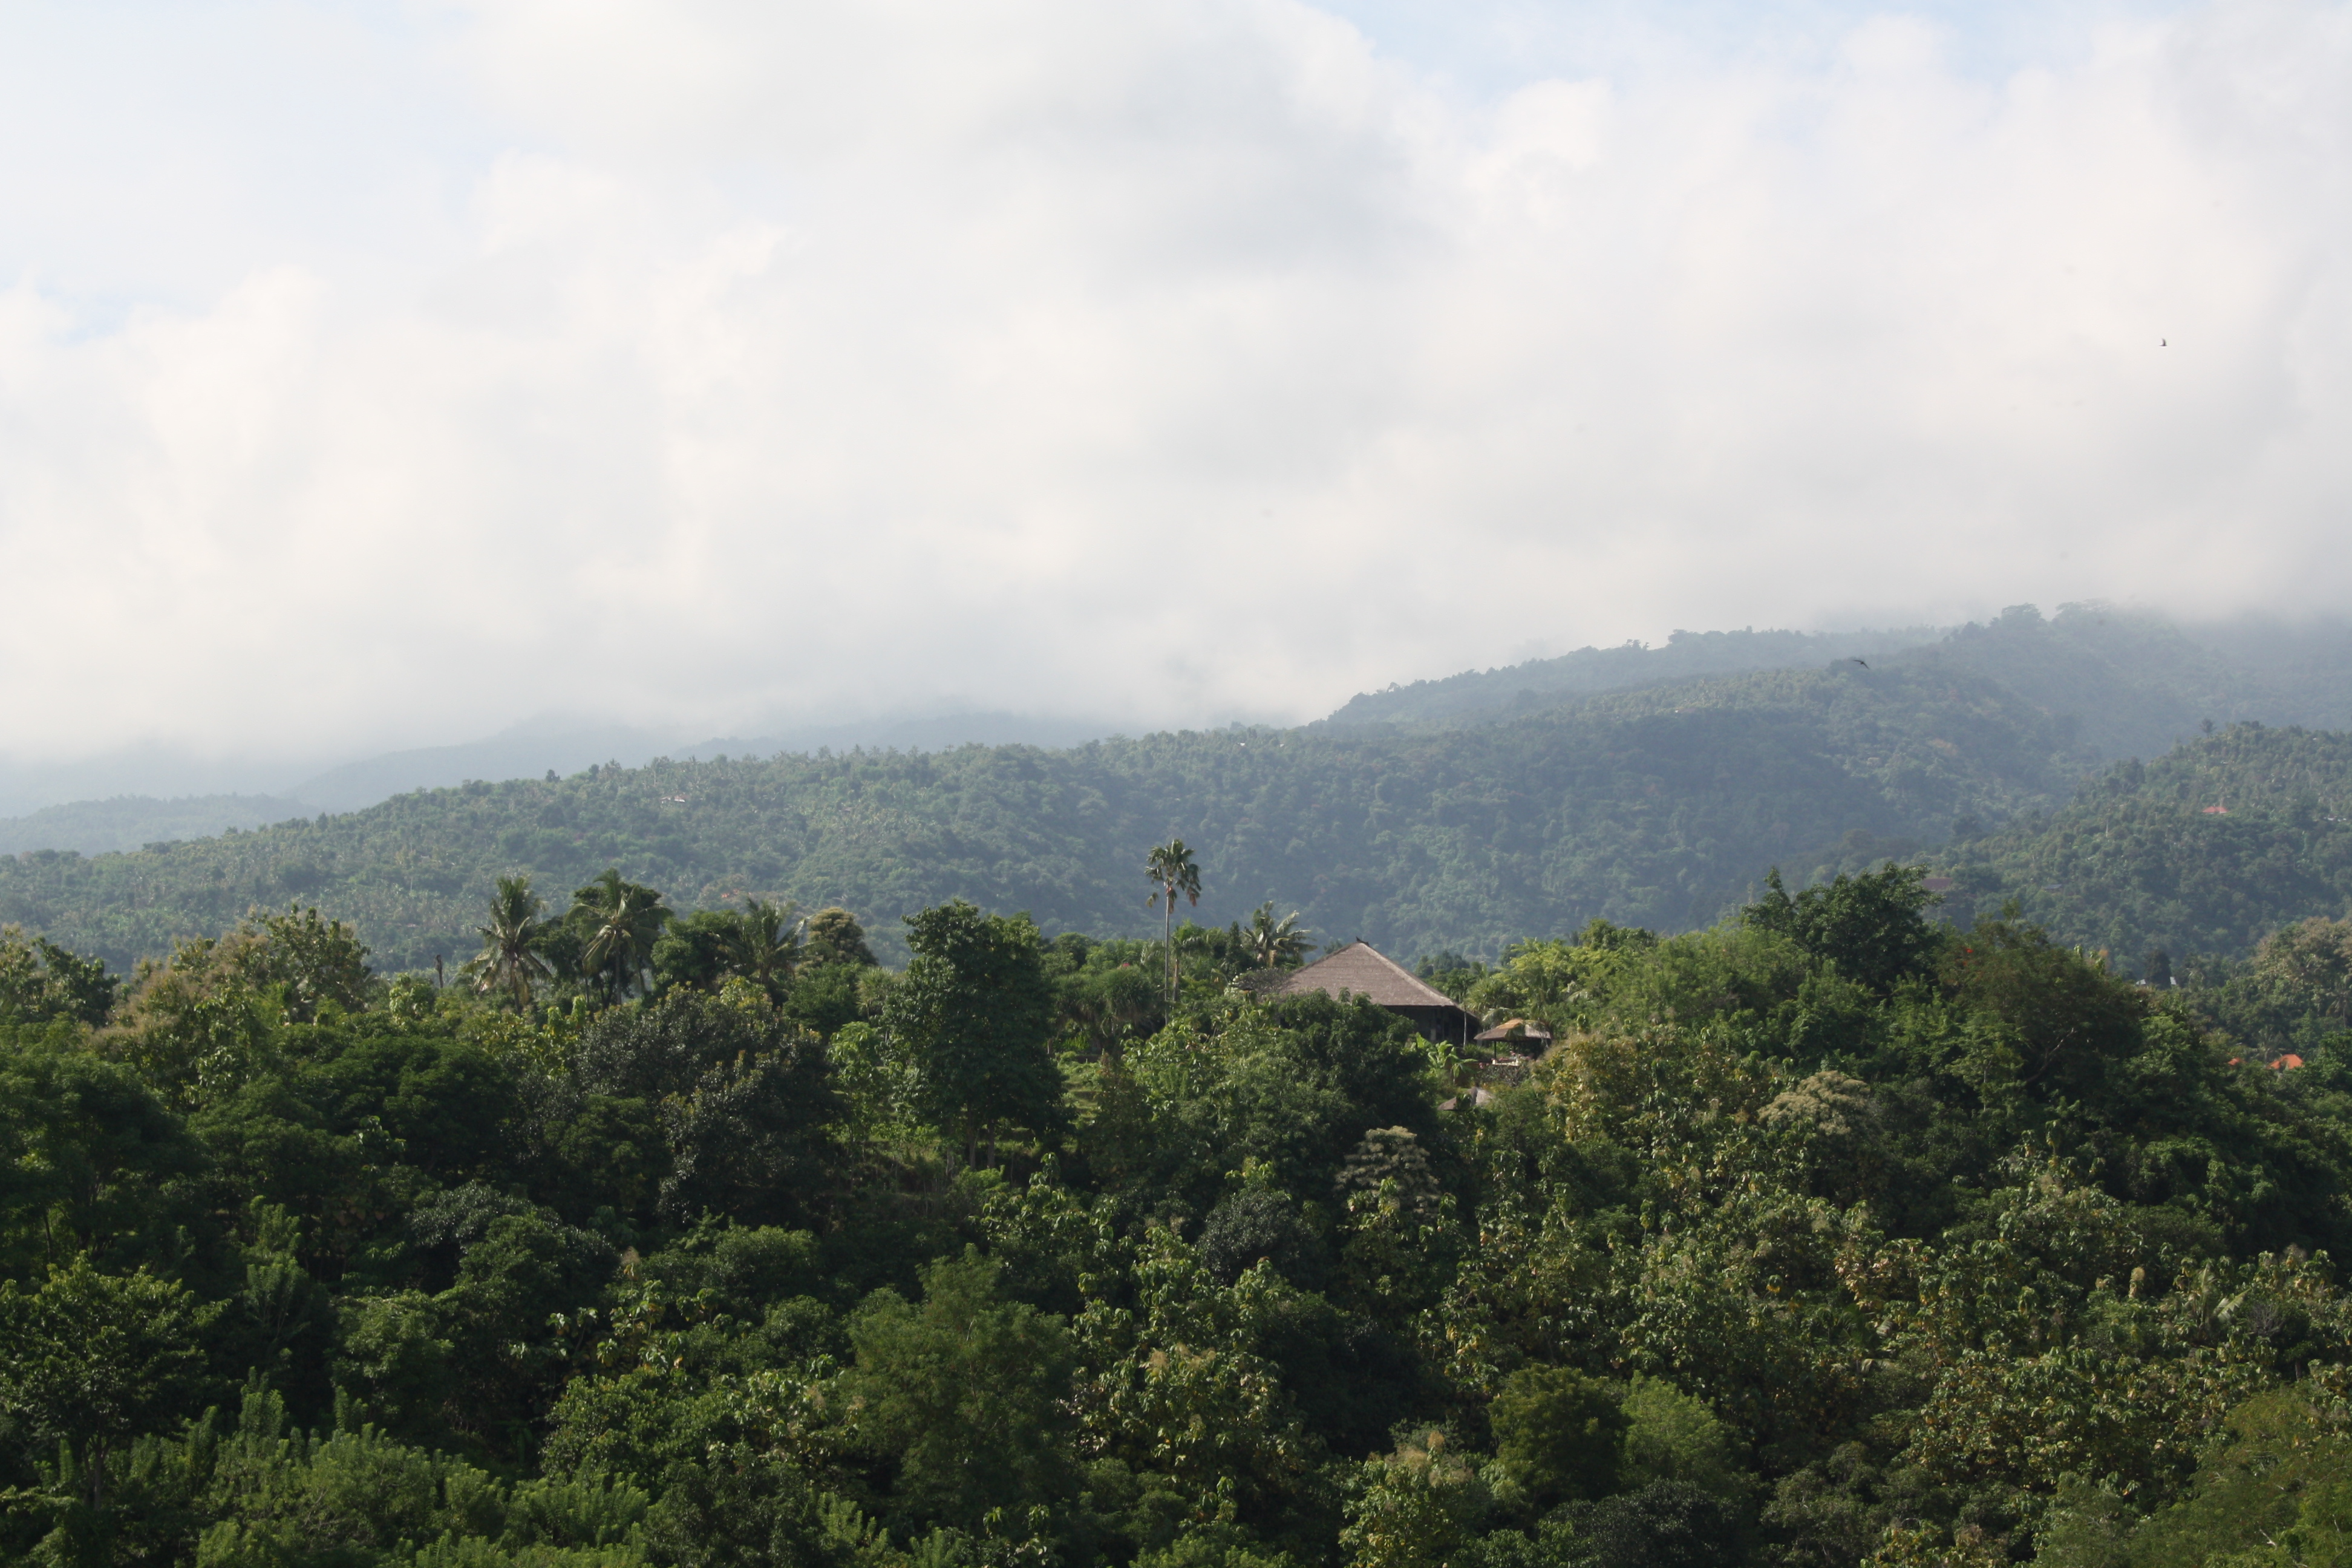
\includegraphics[width=15cm]{pics/landscape1.jpg}
\caption*{Mixed use tropical landscape in Bali.}
\end{figure}

\pagebreak

\section{Abstract}\label{abstract-4}

To survive in a warming world the range of many species will shift
polewards or upwards. Tropical rainforests harbour most of the world's
remaining terrestrial biodiversity, included many thermally restricted
forest specialists. Despite this, we currently lack a biome-wide
assessment of the potential for tropical species to reach climate
analogues within existing forest cover. Moreover, no study to date has
empirically tested where, how and why climate connectivity has changed
as a result of change in forest cover. In this study, we quantified
pantropical climate connectivity in 2000 and 2012. We tested various
hypotheses relating climate connectivity change to the magnitude and
location of forest cover change. We found that\ldots{} To conserve
global biodiversity under climate change, we suggest that unavoidable
forest loss in the tropics should be\ldots{}, and that forest protection
and reforestation should\ldots{}

\section{Introduction}\label{introduction-3}

To avoid extinction under future climate change, species must either
adapt \emph{in situ} or shift their range \citep{hobbs_movers_2018}.
Both strategies have been widely studied, with range shifts polewards or
upwards appearing to be a widespread response to climate change across
the globe, in both palaeoecological records and under modern climate
change \citep{parmesan_ecological_2006, davis_range_2001}, and across a
range of taxa
\citep{chen_elevation_2009, freeman_rapid_2014, raxworthy_extinction_2008}.
There is potential for other human impacts, including land-use change,
to influence the ability of species to shift their ranges in response to
climate change. Understanding such interactions is a conservation
priority
\citep{brook_synergies_2008, mantyka-pringle_interactions_2012, sirami_impacts_2017, titeux_global_2017}.

Land-use change impedes range shifts in most cases, by creating highly
fragmented landscapes through which many species struggle to navigate
\citep{thomas_extinction_2004, heller_biodiversity_2009, tucker_moving_2018}.
The tropics is an area of particular concern because it harbours most
remaining terrestrial biodiversity \citep{jenkins_global_2013} while
also being the focus of intensive and extensive land-use change via the
conversion and degradation of tropical forests
\citep{hansen_high-resolution_2013, lewis_increasing_2015}. Although the
absolute magnitude of climate change will be greatest at the poles
\citep{ipcc_climate_2013}, long periods of climatic stability mean that
is the tropics where relative climate change will be the most severe
\citep{mora_projected_2013}. Many tropical species have limited
tolerance for temperature change
\citep{deutsch_impacts_2008, tewksbury_putting_2008, khaliq_global_2014},
and are also highly sensitive to fragmentation because of habitat
specialism and poor dispersal ability \citep{opdam_climate_2004}.
Climate-driven range shifts in the tropics generally follow elevation al
gradients, probably because latitudinal temperature gradients are very
shallow \citep{loarie_velocity_2009}. Range shifts of tropical species
have been documented in response to as little warming as 0.1°C to 0.76°C
\citep{parmesan_globally_2003, raxworthy_extinction_2008, chen_elevation_2009, peh_potential_2007, freeman_rapid_2014, raxworthy_extinction_2008}.

The ability of species to shift their ranges in response to climate
change depends both on the future availability of suitable habitat with
an analogous climate, and the connectivity between the species' current
distribution and any potential future habitat. Species Distribution
Models (SDMs) have been key in addressing the former, using the
correlation between current distribution and current abiotic conditions
(including climate) to forecast where species might go in the future
\citep{hijmans_ability_2006}. However, not only do SDMs fail to consider
connectivity, they are also fine-filter approaches focusing on specific
species and requiring a wealth of data relating to the distribution of
those species \citep{nunez_connectivity_2013}. Equally, there is a
plethora of studies that quantify habitat connectivity -- both
structural and actual connectivity
\citep{calabrese_comparison-shoppers_2004} -- which have been
instrumental in highlighting the extent of fragmentation by land-use
change
\citep[e.g.][]{tucker_moving_2018, brodie_evaluating_2015, cosgrove_consequences_2017}.
These studies, however, do not explicitly consider climate. This is
important because large areas of structurally connected habitat could
still become unsuitable under climate change if there is insufficient
climatic heterogeneity within that habitat (e.g.~lowland rainforest).

The handful of studies that do integrate habitat connectivity with
climate are highly informative both for quantifying the current
connectedness of natural areas to future climate analogues, and for
predicting specific movement routes or `climate corridors' between
source and target areas
\citep{mcguire_achieving_2016, littlefield_connecting_2017, nunez_connectivity_2013}.
Such corridors could prove vital for many range-shifting species. That
said, `climate connectivity', defined as the extent to which ``spatial
configuration of natural lands allows species to track their current
climatic conditions during projected climate change''
\citep{mcguire_achieving_2016}, has yet to be reviewed for a whole
biome, nor has any study to date utilised empirical data to examine the
change in climate connectivity over time. The latter is significant if
we are to understand the factors that drive change in climate
connectivity: where does an increase in natural habitat maximise climate
connectivity, and where does loss of natural habitat minimise loss of
climate connectivity?

In this study, we combined current and future climate data with data
from tropical land-use change that has already occurred, to quantify
both the current climate connectivity across the tropics and the
patterns of climate connectivity change in the recent past. To enable a
broad, coarse-filter assessment of climate connectivity, we consider
land use only in terms of forest versus non-forest, using 2000 and 2012
tree cover data from \citet{hansen_high-resolution_2013} and excluding
tree plantations \citep{transparent_world_tree_2015}. Climate
connectivity was quantified by adapting the approach of
\citet{mcguire_achieving_2016}: forested areas were categorised into
patches according to 0.5°C increments in Mean Annual Temperature
\citep{hijmans_very_2005}, and for each patch we calculated the coolest
destination patch that could be reached by traversing a gradient from
hotter to cooler adjacent patches. Patches achieved climate connectivity
if they were able to reach a destination with a future temperature
cooler than or equal to its current temperature. The aim of this
approach is to quantify only the physical potential for
thermally-restricted tropical forest species to reach climate analogues
via forested habitat; it does not take into account any species-specific
restrictions such as dispersal distance. We hypothesised that forest
cover change from 2000 to 2012, elevation and the geometry of forest
patches (patch area) would explain much of the variation in climate
connectivity.

\section{Materials and Methods}\label{materials-and-methods}

We focused our study on the pantropics, including all land masses
located between ±23.43694° latitude and more than 65,610
km\textsuperscript{2} in area {[}\emph{this is to reduce computational
load and focus on places where range shifts are likely to be most
feasible - it's currently arbitrarily set as the area of Sri Lanka}{]}.
Maps were analysed at 1-km resolution projected into the World
Cylindrical Equal Area projection. All spatial layers were processed
with Python code implemented using the arcpy module in ArcMap version
10.4.1 \citep{esri_arcgis}.

\subsection{Climate-partitioned forest
patches}\label{climate-partitioned-forest-patches}

Since we were interested in climate connectivity for tropical forest
specialists, we calculated climate connectivity based on movement along
a temperature gradient within forested areas only. We defined regions as
forest or non-forest using tree cover data from
\citet{hansen_high-resolution_2013}. For the year 2000 (the recent past)
cells were defined as forested if they had \textgreater{} 50\% tree
cover \citep{hansen_high-resolution_2013}, and did not fall within the
boundaries of tree plantations \citep{transparent_world_tree_2015}. For
the year 2012 (present day), cells were classed as forest based on
forest loss and forest gain \citep{hansen_high-resolution_2013} relative
to the forest cover in 2000. If a cell had experienced forest loss from
2000 to 2012, it had gone from a forested to non-forested state and the
cell was classed as non-forest. Conversely, if a cell had experienced
forest gain from 2000 to 2012, it had gone from a non-forested to
forested state; providing there had been no loss and the cell was not
within a tree plantation, the cell was classed as forest.

Based on the approach of \citet{mcguire_achieving_2016}, we partitioned
forest patches using a present-day (\textasciitilde{}1950-2000),
30-arc-second global layer for Mean Annual Temperature (hereafter:
temperature) from the WorldClim database \citep[Version
1.4;][]{hijmans_very_2005}, resampled to 1 km\textsuperscript{2}. The
same approach was applied separately to 2000 forest cover and 2012
forest cover: temperature values were assigned to forested cells and
reclassified to increments of 0.5°C, based on evidence that tropical
species are sensitive to this degree of temperature difference
\citep[e.g.][]{peh_potential_2007, freeman_rapid_2014, raxworthy_extinction_2008}.
The resulting raster was then converted to polygons, whereby
neighbouring forest cells with the same temperature value were assigned
to the same polygon (hereafter: forest patch). While our approach is not
specific to any particular taxon, it may be helpful to consider it in
the context of range shifts by non-volant terrestrial animals
\citep[cf.][]{nunez_connectivity_2013}. We removed forest patches
\textless{} 10 km\textsuperscript{2} in area, based on the assumption
that they could not support a population for long enough to enable range
shifts {[}REF{]}. Patches within 2 km of each other were assigned to the
same patch, assuming that populations could move across 2 km of
non-forest to reach suitable habitat {[}REF{]}.

\subsection{Climate connectivity}\label{climate-connectivity}

The logic behind the measure of climate connectivity in
\citet{mcguire_achieving_2016} is that it represents the maximum
temperature differential between current and future conditions that can
be achieved by traversing a gradient of hotter to cooler patches within
existing forest cover. We assigned mean current and future temperature
to all forest patches, again using data from WorldClim. Future
temperature was for the year 2050 (2041-2060), derived from the
HadGEM2-AO general circulation model \citep{ipcc_climate_2013} and
Representative Concentration Pathway (RCP) 8.5, which is the most severe
(`business-as-usual') IPCC scenario.

To trace each forest patch to its final destination patch we identified
which patches were neighbours, and - for each neighbour pair - defined
the hotter patch as the origin and the cooler patch as the destination.
Most patches will have multiple neighbours, creating a network of
connected patches with many possible pathways between them. We iterated
over each unique temperature from cooler to hotter, propagating cool
temperatures backward through the network of connected patches to
identify the coolest temperature that could be reach for each origin
patch \citep[see Supplementary Text 1 for a worked
example;][]{mcguire_achieving_2016}.

Once each origin patch has a designated final destination patch, climate
connectivity is calculated from the temperature differential between
them. The key question is whether forest cover is sufficient for
organisms to reach a place that, under future climate warming, is the
same as or cooler than the temperature where it currently resides. Thus,
climate connectivity is simply current temperature of the origin patch
minus the future temperature of the destination patch. Where this value
is zero or positive, the patch has achieved climate connectivity: there
is sufficient structural connectivity between forested areas for
organisms to reach an analogous future climate.

Climate connectivity was necessarily calculated at a patch-level,
independently, for 2000 and 2012. However, because patches themselves
were not constant through time, we used median climate connectivity
within 50 m elevation al bands as our response variable. This not only
enables comparison between the years, but also captures the potential
interacting effect of elevation. Most human development occurs at lower
elevations and most tropical species will likely track temperature
gradients by moving uphill \citep{loarie_velocity_2009}, therefore both
the patterns and significance of climate connectivity are likely to vary
according to elevation. Elevation was derived from NASA's SRTM 90m
Digital Elevation Database v4.1 \citep{nasa_srtm_2008}.

\subsection{Statistical analyses}\label{statistical-analyses-1}

All data were analysed using linear models in R version 3.4.3
\citep{r_core_team_2017}. To understand current patterns we modelled
2012 climate connectivity against both elevation and continent. Any
continental differences in climate connectivity are important from a
policy perspective, but may also be expected owing to the different
biogeography and land-use history of each continent within the
pantropics: North and South America (hereafter: Latin America), Africa,
Asia and Australia.

We hypothesised that the key drivers of change in climate connectivity
would be change in forest cover and the geometry of forest patches in
the year 2000. Within the same elevation al bands used to define climate
connectivity, we calculated median patch area (km\textsuperscript{2}) in
the year 2000 (henceforth: patch area) and the total number of cells
that went from a forested to non-forested state between 2000 and 2012
(henceforth: forest loss). In the full model, we tested change in
climate connectivity against elevation and forest loss (and the
interaction between them), and against patch area.

\section{Results}\label{results-3}

\subsection{Current state of climate
connectivity}\label{current-state-of-climate-connectivity}

Across the whole study area, climate connectivity in 2012 ranged from a
minimum of ??°C to a maximum of ??°C, with a median value of??°C. Only
??\% of the total area of forest patches achieved successful climate
connectivity, with a value more than or equal to zero (Figure
\ref{fig:fig-1}). Climate connectivity differed substantially by
elevation band (F = ??; P = ??), initially decreasing sharply as
elevation increased, before reaching a plateau of around -3°C at
elevations of 100 m or more (Figure \ref{fig:fig-2}).

\subsection{Change in climate
connectivity}\label{change-in-climate-connectivity}

Many areas experienced no change in climate connectivity from 2000 to
2012 (Figure \ref{fig:fig-3}), although change ranged from ??°C to
+??°C. Forest loss was widespread, with a total area of ??
km\textsuperscript{2} deforested between 2000 and 2012 (Figure
\ref{fig:fig-4}).

Change in climate connectivity over time was unaffected by the area of
forest patches in the year 2000 (F = ??; P = ??), but decreased with
increasing forest loss (F = ??; P = ??; Figure \ref{fig:fig-5}).

\section{Discussion}\label{discussion-3}

\begin{itemize}
\tightlist
\item
  We quantify for the first time the state of climate connectivity
  across the tropics, and how it has changed over a 12-year period.
\item
  We make use of global datasets to empirically test factors that
  influence the probability of forest gaining or losing climate
  connectivity, such as the magnitude of forest cover change and
  elevation.
\item
  \emph{Interpretation of predictors of climate connectivity and change
  in climate connectivity, and what this means for biodiversity.}
\item
  Quantifying and understanding climate connectivity in the tropics is
  important for estimating the potential for thermally-restricted forest
  specialists to adaptively respond to climate change. Such species
  represent a large proportion of the world's total biodiversity, but
  are highly threatened and highly vulnerable.
\end{itemize}

\subsection{Caveats and limitations}\label{caveats-and-limitations}

It is important to note that we are not quantifying climate connectivity
for particular species. This study is focused on how land-use change and
climate change will interact to affect groups of species with particular
thermal requirements. As such, our protocol analyses how forest cover
and forest cover change affects the physical connectedness of forest
patches within a particular climatic niche
\citep[cf.][]{mcguire_achieving_2016}. The measure of climate
connectivity is essentially a measure of the potential for
thermally-restricted groups of species to track their preferred climate
through near-continuous forest cover; we do not suggest that this alone
is sufficient to predict the likelihood that such species will be
capable of avoiding extinction under climate change. Many other factors
will affect both the need and capacity for species to shift their ranges
in response to rising temperatures. For example, even
thermally-restricted species can adapt \emph{in situ} via phenotypic
plasticity, genetic adaptation or exploitation of climate refugia
\citep{parmesan_ecological_2006, hannah_fine-grain_2014}.
Species-specific factors such as dispersal limits could preclude species
from tracking their preferred climate even where climate connectivity
exists, while some species may be capable of traversing greater
distances through non-forest than we have allowed in our approach.

We focus on Mean Annual Temperature to create climate-partitioned forest
patches, but note that other climate variables -- particularly
precipitation -- are also extremely important in determining the
climatic niche of any given species. Unfortunately, projections of
future precipitation under climate change remain highly uncertain
\citep{ipcc_climate_2013, corlett_climate_2012}, and are also highly
variable in space, both of which make it unclear the gradient that
species would have to follow to avoid deleterious changes in
precipitation.

The breadth of our study enabled us to determine broad trends and
patterns across the most biodiverse biome in the terrestrial realm.
However, to achieve such breadth requires that assumptions and
simplifications are made. Our results should not be used to infer
regional and local climate connectivity directly, but rather as a
signpost to locations that appear to deviate from trends at a
pantropical scale, and would therefore benefit from further, targeted
investigation at a finer spatial scale, potentially incorporating
species-specific information appropriate to the questions of interest
\citep[e.g.][]{martensen_spatio-temporal_2017}. Violations of our
assumptions in particular regions would, of course, render our estimates
of climate connectivity less accurate in those places. Overall, however,
our focus is on climate connectivity at a pantropical scale, and
therefore regional discrepancies will likely have limited impact on our
overall conclusions. Our study, along with other, similar studies
\citep{mcguire_achieving_2016, martensen_spatio-temporal_2017, nunez_connectivity_2013},
represents the first steps towards capturing the current state of
climate connectivity, but inevitably these approaches will be greatly
enhanced by continuing developments in computational power and global,
remotely-sensed datasets \citep{sanchez-azofeifa_twenty-first_2017}.

\subsection{Summary}\label{summary-1}

Assessing the current status of climate connectivity across a whole
biome enables us to establish a baseline, against which we can better
appreciate the current and future threats to global biodiversity from
the combined influence of land-use change and climate change. By using
empirical data to characterise where, how and why forest cover change
impacts climate connectivity, we can ensure that landscape planning of
future, unavoidable forest loss is done with climate resilience in mind.
Similarly, we can plan for forest gain (i.e.~reforestation) and forest
protection (e.g.~Protected Areas) that incorporates and enhances climate
corridors.

\chapter{Discussion}\label{discussion-4}

\begin{figure}[!htb]
\centering
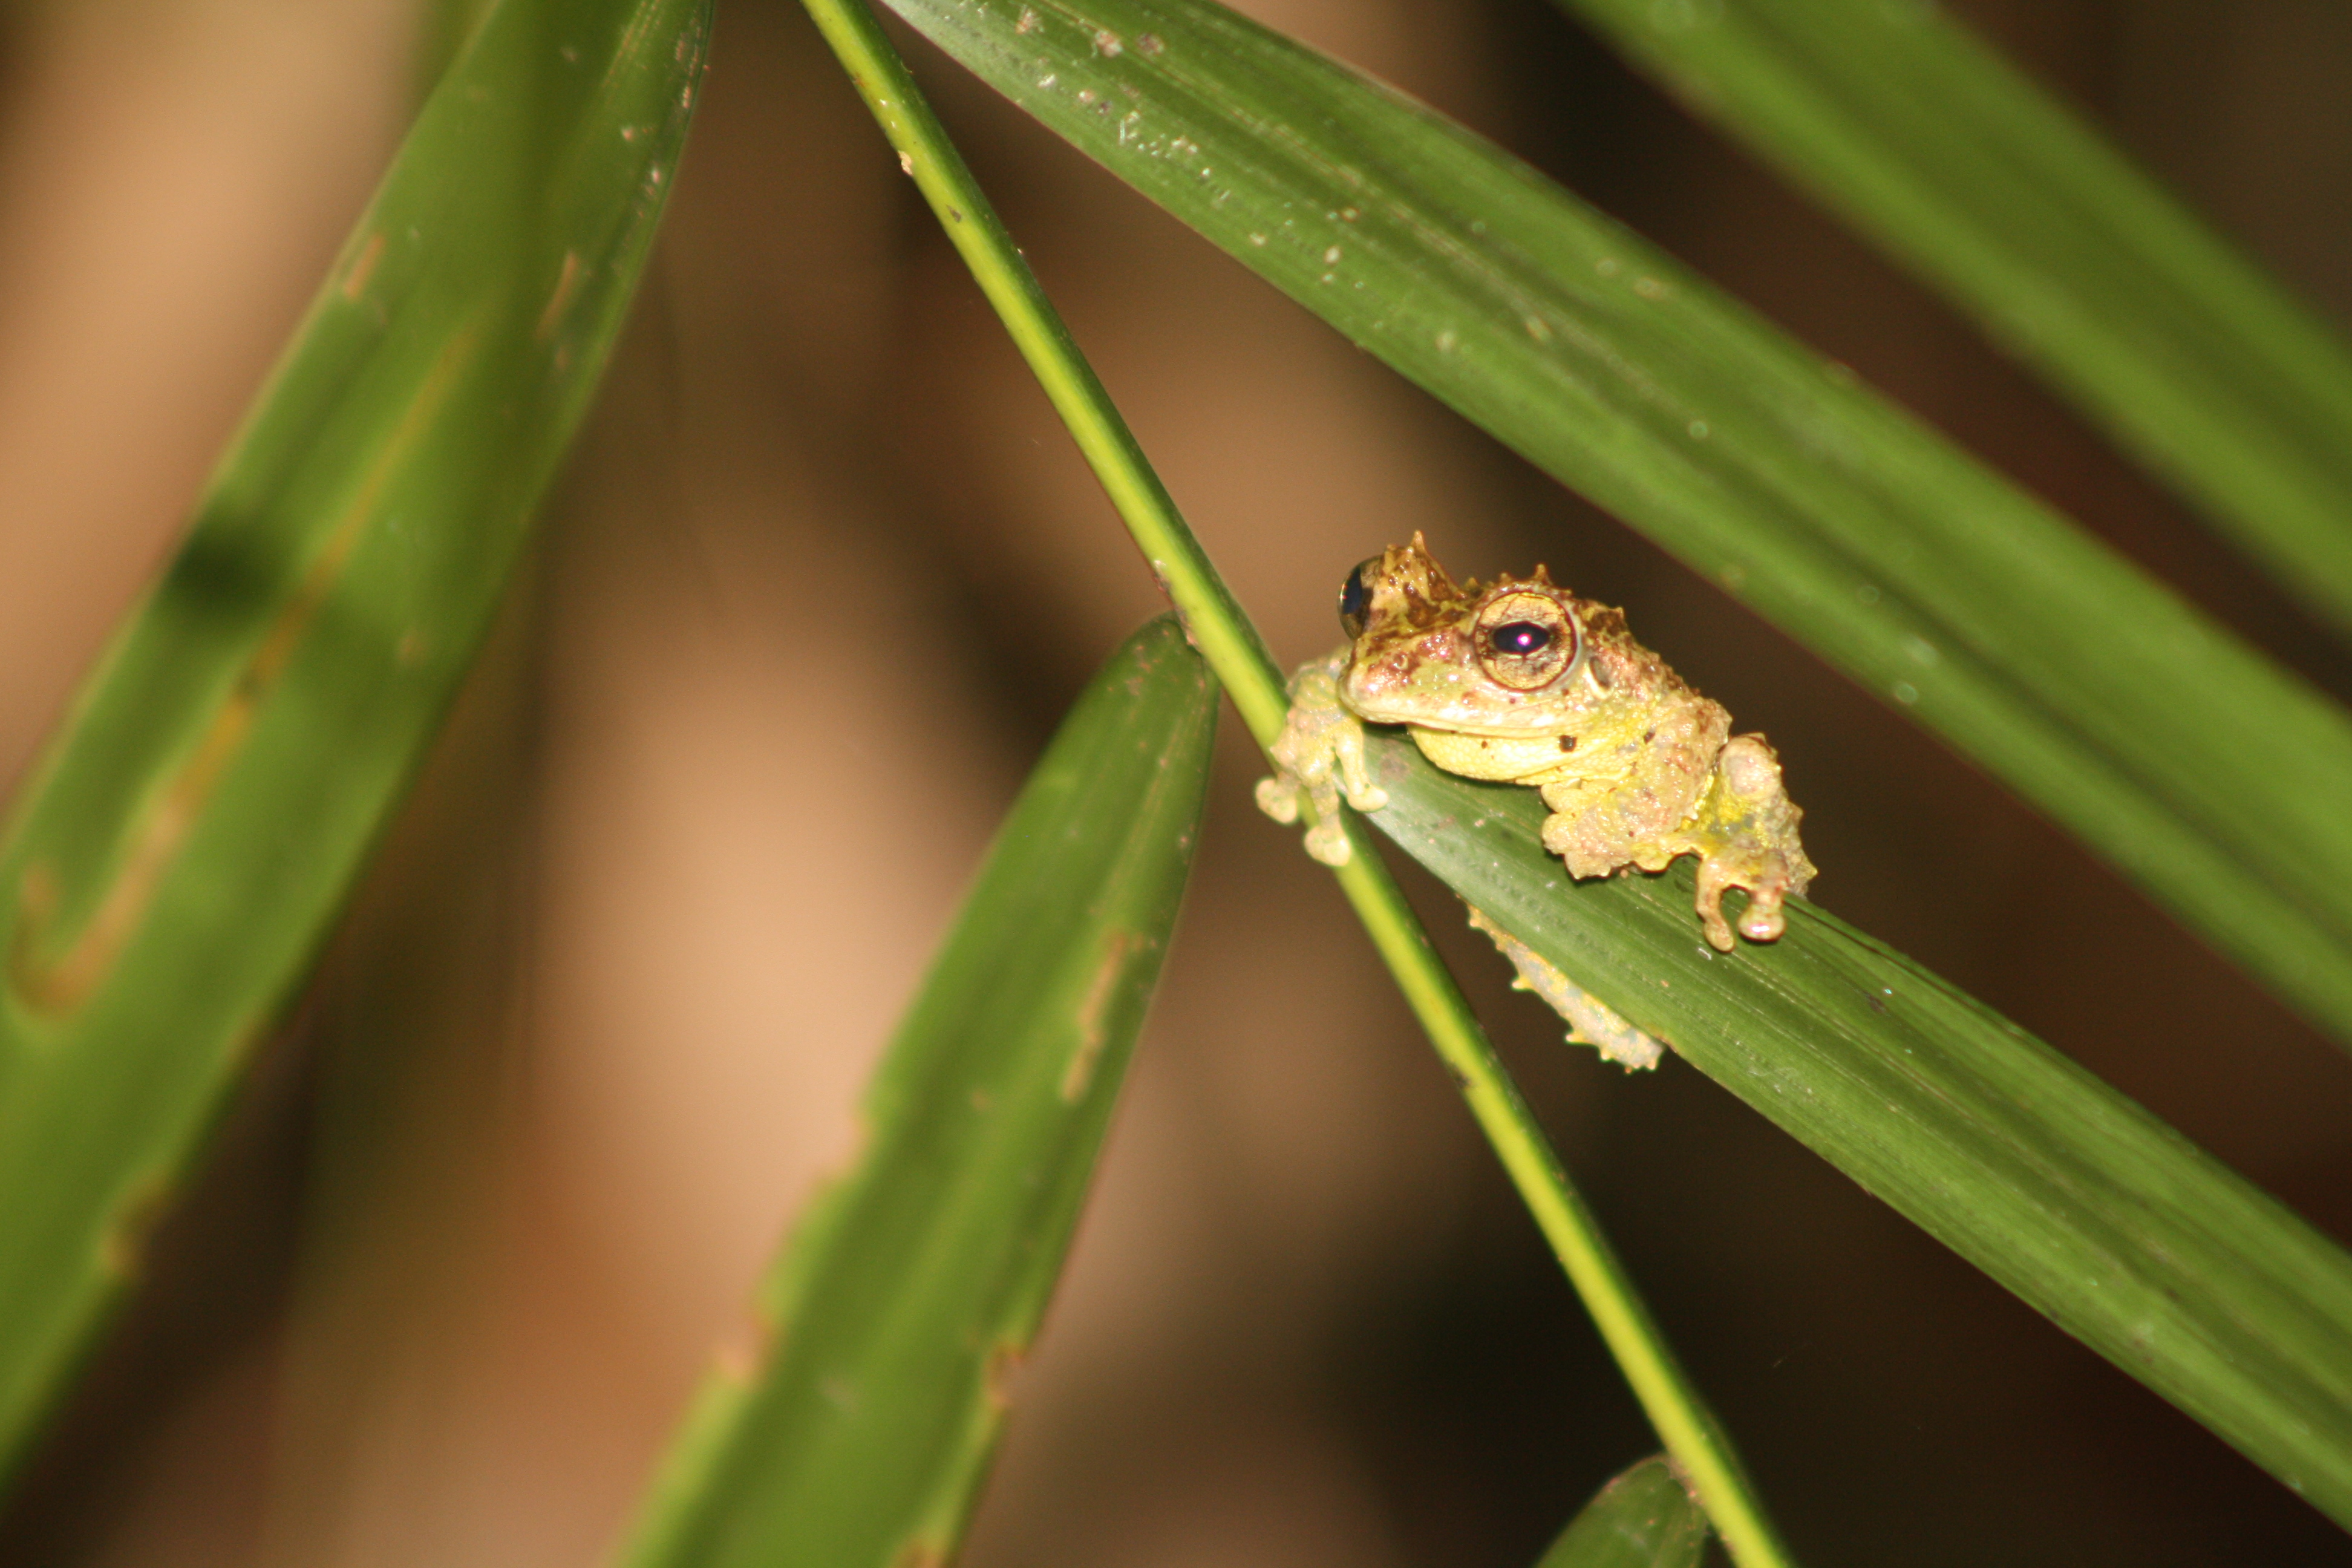
\includegraphics[width=13cm]{pics/Frilled_tree_frog.jpg}
\caption*{Frilled tree frog (\textit{Kurixalus appendiculatus}).}
\end{figure}

\section{Summary of thesis findings}\label{summary-of-thesis-findings}

\begin{itemize}
\tightlist
\item
  Aims of thesis were:

  \begin{enumerate}
  \def\labelenumi{\arabic{enumi}.}
  \tightlist
  \item
    Investigate the potential for land-use change to impact
    microclimates and microhabitats, and hence the subsequent impacts
    on:

    \begin{itemize}
    \tightlist
    \item
      The baseline of local climate change that global climate change is
      projected onto
    \item
      The potential for thermal buffering as an adaptive response
    \end{itemize}
  \item
    Investigate the potential for land-use change to impact range shifts
    under climate change
  \end{enumerate}
\end{itemize}

\textbf{Chapter 2 -- A pantropical analysis of the impacts of forest
degradation and conversion on local temperature}

** Main objectives:** 1. 2. 3. * Assessed how degradation and conversion
of tropical forests directly impacts temperature on a fine
spatiotemporal scale * Implications for the impact of further warming
under global climate change, but suggests that degraded forests and
microhabitats may be able to buffer species from further change

\textbf{Chapter 3 -- A framework for quantifying fine-scale thermal
heterogeneity in the field}

** Main objectives:** 1. 2. 3. * Developed software and metrics for
analysing thermal images * Enables other researchers to more easily
utilise thermography as a technique for researching thermal regimes,
which are vitally important to species' ecology

\textbf{Chapter 4 -- Tropical forests are thermally buffered despite
intensive selective logging} ** Main objectives:** 1. 2. 3. * Compared
fine-scale temperature in primary and selectively logged forests of
Borneo, using field data collected with dataloggers and a thermal camera
* Found that despite clear structural differences between these forest
types, there was very little temperature variation which suggests rapid
thermal recovery and underscores the importance of logged forests for
biodiversity both now and under future climate change

\textbf{Chapter 5 -- The impact of recent forest cover change on climate
connectivity in the tropics}

** Main objectives:** 1. 2. 3. * Combined global tree cover and climate
datasets to quantify, pantropically, the current physical potential for
species to reach climate analogues through near-continuous forest, and
the extent to which this has been affected by recent forest cover change
* Found that current levels of climate connectivity are generally very
poor, particularly in lowland regions with low forest cover and on
mountain summits, hence many tropical species will struggle to reach
analogous climate given current levels of forest cover

\section{Climate at the fine scale}\label{climate-at-the-fine-scale}

\begin{itemize}
\tightlist
\item
  Chapter 2 highlights that climate at the very coarse scale can mask
  important patterns occurring at a local scale

  \begin{itemize}
  \tightlist
  \item
    Land-use change has a direct impact on local climate
  \item
    Suggestion that below-ground and within degraded forests species may
    avoid direct warming that results from loss of forest cover
  \item
    Bias towards particular regions \& LUT
  \item
    Doesn't account for intensity
  \end{itemize}
\item
  Chapter 3 establishes a framework to assess thermal regimes at an even
  finer spatial scale, using thermography

  \begin{itemize}
  \tightlist
  \item
    Importance of very fine spatial scale
  \item
    Importance of surface temperature
  \item
    Importance of spatial temperature variation
  \end{itemize}
\item
  Chapter 4 applies the framework of Chapter 3, alongside traditional
  dataloggers cf.~Chapter 2, to further explore the potential for
  thermal buffering in selectively logged forests of Borneo

  \begin{itemize}
  \tightlist
  \item
    Confirm that local temperature is unaffected by selective logging,
    but so too is the fine-scale temperature variation that is vital for
    thermal buffering by animasls
  \end{itemize}
\item
  Neither approach considered other climatic variables that are
  important to species' ecology under climate change (e.g.~water \&
  wind)
\item
  Should also consider the vertical climate gradient in tropical
  rainforest \citep{scheffers_tropical_2018, scheffers_vertical_2017}
\end{itemize}

\section{Climate at the coarse scale}\label{climate-at-the-coarse-scale}

\begin{itemize}
\tightlist
\item
  Fine-scale climate is important for the day-to-day, individual-level
  responses of organisms to suboptimal temperatures, but over decades it
  is highly likely that many species will respond to coarse-scale
  climate change by shifting their ranges

  \begin{itemize}
  \tightlist
  \item
    This could happen alongside in situ adaptation, which could provide
    a buffer and allow more time for species to reach new target habitat
  \item
    It could also be that in situ adaptation is not possible or is
    insufficient, for example in converted lands where the local
    temperature has increased to a level way beyond the thermal
    tolerance of forest specialists
  \end{itemize}
\item
  Chapter 4 considers the extent to which land-use change impacts
  landscape permeability, and the subsequent potential for species to
  reach analogous climates through natural habitat

  \begin{itemize}
  \tightlist
  \item
    Current levels of forest cover in the tropics offer poor
    connectivity between analogous climates, which has largely worsened
    from 2000 to 2012
  \end{itemize}
\item
  Only considering structural connectivity - no species data (this would
  make the approach species-specific and impose data limitations)
\item
  Do not consider other climate variables, because their projections are
  uncertain and spatially variable, which makes it impossible at this
  stage to determine the gradient that species would have to follow to
  maintain climate parity
\end{itemize}

\section{Wider applicability of
findings}\label{wider-applicability-of-findings}

\subsection{Biological relevance}\label{biological-relevance}

\begin{itemize}
\tightlist
\item
  Chapters 2-4 are most relevant to small-bodied ectotherms, that are
  heavily influenced by local and fine-scale temperature and which are
  widely known to utilise thermal variation at this scale as a means to
  avoid suboptimal climatic conditions at a coarser scale

  \begin{itemize}
  \tightlist
  \item
    Also relevant to small-bodied endotherms, although less is known
    about the extent to which they can and do utilise microclimates in
    tropical forests
  \item
    Could be relevant to plants, particuarly in early life stages
    e.g.~germination
  \item
    A need to consider how behavioural exploitation of fine-scale
    temperature variation interacts with local adaptation and
    acclimation, and coarser scale responses such as range shifts
  \end{itemize}
\item
  Chapter 5 is more relevant to larger and more mobile animal species,
  such as medium-sized mammals, which are perhaps less able to adapt in
  situ but likely to shift their ranges in response to climate change

  \begin{itemize}
  \tightlist
  \item
    Relevance to plants will also depend on ability to disperse across
    matrix
  \item
    Unknowns about how forest itself will shift under climate change
    also influences the relevance of these results to forest specialists
  \item
    Different kinds of forest, which will limit different species to
    differeng extents
  \item
    Inclusion of tree plantations may not be appropriate for many forest
    specialists, since they tend to lack structural and biological
    diversity
  \end{itemize}
\end{itemize}

\subsection{Relevance across tropics}\label{relevance-across-tropics}

\begin{itemize}
\tightlist
\item
  Chapter 2 was pantropical, but Africa was poorly represented

  \begin{itemize}
  \tightlist
  \item
    Where natural vegetation is not forest (e.g.~parámo, cerrado,
    savannah, dessert), it is expected that land-use change will have a
    much less substantial impact on local temperature
  \end{itemize}
\item
  Chapter 4 focused on a region of the tropics where logging intensity
  has in the past been very severe, but where logging activity has since
  ceased

  \begin{itemize}
  \tightlist
  \item
    Less relevant to areas with ongoing intensive logging
  \item
    Less relevant to areas where recovery of canopy cover has not been
    permitted or not possible
  \end{itemize}
\item
  Chapter 4 only focused on the understorey, but in vertically complex
  forests there may well me a different result above the understorey
\end{itemize}

\section{Recommendations for conservation and futher
research}\label{recommendations-for-conservation-and-futher-research}

\begin{itemize}
\tightlist
\item
  Land-use change is still a primary cause of species loss, and the lack
  of consideration of climatic impacts of land-use change may have
  underestimated this impact or caused it to be confounded with climate
  change (Chapter 2)
\item
  Growing literature on the ways in which land-use change and climate
  change interact, but the impacts on risk of extinction for particular
  species will depend on many factors:

  \begin{itemize}
  \tightlist
  \item
    Spatiotemporal scale (Chapter 3 and 4)
  \item
    Plasticity
  \item
    Local adaptation
  \item
    Functional connectivity (e.g.~dispersal limits, metapopulation
    dynamics)
  \end{itemize}
\item
  On a local scale, enhancing thermal heterogeneity may help species to
  thermoregulate and so buffer species from climate change (at least
  offering them more time to adpat or disperse)

  \begin{itemize}
  \tightlist
  \item
    Chapter 4 suggests that natural resoration over a decade is
    sufficient for thermal recovery in the understorey, but this should
    be integrated with recovery of other abiotic and biotic requirements
  \item
    More research is needed on the speed of thermal recovery, and
    whether active restoration or RIL techniques might have a role to
    play in enhancing thermal recovery from logging
  \end{itemize}
\item
  With improvements in technology, it would be fruitful to consider:

  \begin{itemize}
  \tightlist
  \item
    Other climatic factors, particularly moisture, at a fine spatial
    scale
  \item
    Linking different spatiotemporal scales e.g.~combining thermal
    imagery with drones to characterise thermal landscapes more
    extensively, or developing correlative models to link subcanopy
    climate to remotely sensed temperature data e.g.~LAI
  \end{itemize}
\item
  Chapter 5 emphasises that habitat fragmentation has had a huge impact
  on the structural potential for range shifts, so future conservation
  efforts should aim to deforest, reforest and protect forest with
  climate connectivity in mind

  \begin{itemize}
  \tightlist
  \item
    Particularly hot and cold spots of climate connectivity can be used
    to pursue this research area in finer detail, considering particular
    taxonomic groups and habitat types, and could use scenarios to
    forecast further changes to climate connectivity from changes in
    land use and land cover
  \item
    Again, restoration and protection of degraded forests likely has a
    key role to play in achieving climate connectivity across the
    tropics, while improving conditions in other elements of the matrix
    may also help some species (although this is unlikely to be of net
    benefit if used in place of a land-sparing strategy)
  \end{itemize}
\end{itemize}

\section{Conclusions}\label{conclusions-1}

\begin{itemize}
\tightlist
\item
  The ways in which ongoing degradation and conversion of tropical
  forests impact the ability of species to respond to climate change
  will have a major influence on the long-term viability of forest
  specialists
\item
  Tropical species represent a huge and vulnerable pool of global
  biodiversity, the loss of which would invariably push us towards, and
  perhaps beyond, various plantery boundaries
\item
  We find that land-use change itself can have a major influence on
  climate at the level of the inidvidual, but note that degraded forests
  still provide opportunities for thermal buffering and therefore have
  value both now and under climate change
\item
  Protection of degraded forests, perhaps combined with resoration on
  abandoned agricultural sites, may also help connect species to future
  climate analogues -- something that is clearly needed, since most
  tropical forests already fail to achieve climate connectivity
\item
  In this context, the main aim of land managers should be to maximise
  the options available to species threatened with climate change, and
  so maintain climate resilience within changing tropical landscapes
\end{itemize}

\clearpage
\fancyhead[R]{Appendix \thechapter}

\appendix


\chapter{Supporting information for Chapter
2}\label{supporting-information-for-chapter-2}

\section{Impact of unbalanced sampling}\label{text-A-1}

\subsection{Methods}\label{methods-3}

Some studies contributed substantially more temperature observations
than others. To test whether these studies were unduly influencing our
results, we established a threshold over which a given land-use type, in
a given study, was deemed to have a disproportionate number of
associated temperature observations. The threshold used --- 2,071
observations --- was the mean number of observations across all unique
combinations of land-use type and study identity (55 in total). The same
number of observations (2,071) was then randomly re-sampled from each of
the land-use type and study combinations that exceeded the threshold.
With this reduced and more balanced dataset we repeated the main
analysis (see `Statistical analysis' in main text for more details),
modelling local day-time temperature (`temp\_day') against land-use type
(`LUT'), position relative to ground-level (`position') and season. The
final model structure was unchanged, and included a random slope for
land-use type and random intercept with respect to the identity of the
study (`studyID') from which data originated:

\texttt{lmer(temp\_day\ \ \textasciitilde{}\ LUT*position\ +\ LUT*season\ +\ (LUT\textbar{}studyID))}

\subsection{Results}\label{results-4}

All results were qualitatively unchanged from those derived using the
full dataset. Local day-time temperature was warmer in altered land-use
types, compared to primary forest (LMM, Χ\textsuperscript{2} = 32.19, df
= 4, P \textless{} 0.001; \autoref{fig:fig-A-3}). Averaged across above-
and below-ground, and across seasons, the temperature differential was
greatest in cropland (7.7°C), followed by pasture (6.4°C), plantation
(3.2°C) and degraded forest (0.9°C). The relationship between land-use
type and temperature interacted with both position relative to ground
level (LMM, Χ\textsuperscript{2} = 681, df = 4, P \textless{} 0.001;
\autoref{fig:fig-A-3}a) and season (LMM, Χ\textsuperscript{2} = 105.63,
df = 4, P \textless{} 0.001; \autoref{fig:fig-A-3}b). Specifically, the
difference between altered land-use types and primary forest was greater
above-ground than below-ground (\autoref{fig:fig-A-3}a), and variable
between seasons according to the land-use type (\autoref{fig:fig-A-3}b).

\pagebreak

\section{Supplementary figures}\label{supplementary-figures}













\begin{figure}[H]

{\centering 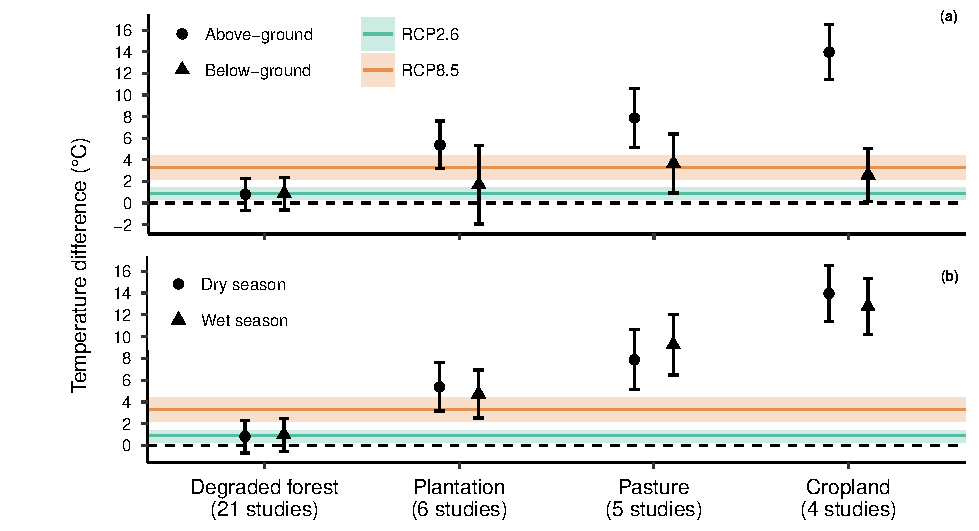
\includegraphics{./output/fig-A-3-1} 

}

\caption{Model estimates of the temperature difference between
altered land-use types and primary forest, using a reduced dataset to
balance sample sizes between the different studies that contributed
data. Parameter estimates are standardised against the estimate for
primary forest, which is represented by the dashed line. Error bars are
95\% confidence intervals. Solid lines indicate projected warming in the
tropics for the period 2081-2100 compared to the period 1986-2005, as a
result of global climate change \citep{ipcc_climate_2013}. Shaded bands
indicate 5\%--95\% ranges from the distribution of the climate model
ensemble. Colours represent the lowest and highest warming scenarios
(RCP2.6 and RCP8.5, respectively).}\label{fig:fig-A-3}
\end{figure}









\begin{figure}[H]

{\centering 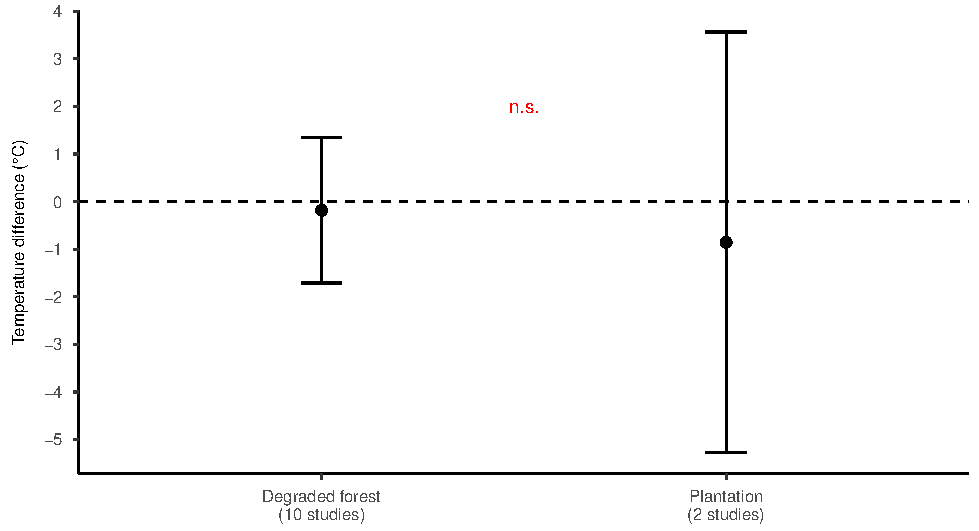
\includegraphics{./output/fig-A-4-1} 

}

\caption{Model estimates of the nocturnal temperature difference
between altered land-use types and primary forest. Note that cropland
and pasture are missing from this analysis because nocturnal temperature
data for these land-use types were not available. Parameter estimates
are standardised against the estimate for primary forest, which is
represented by the dotted line. Error bars are 95\% confidence
intervals.}\label{fig:fig-A-4}
\end{figure}













\begin{figure}[H]

{\centering 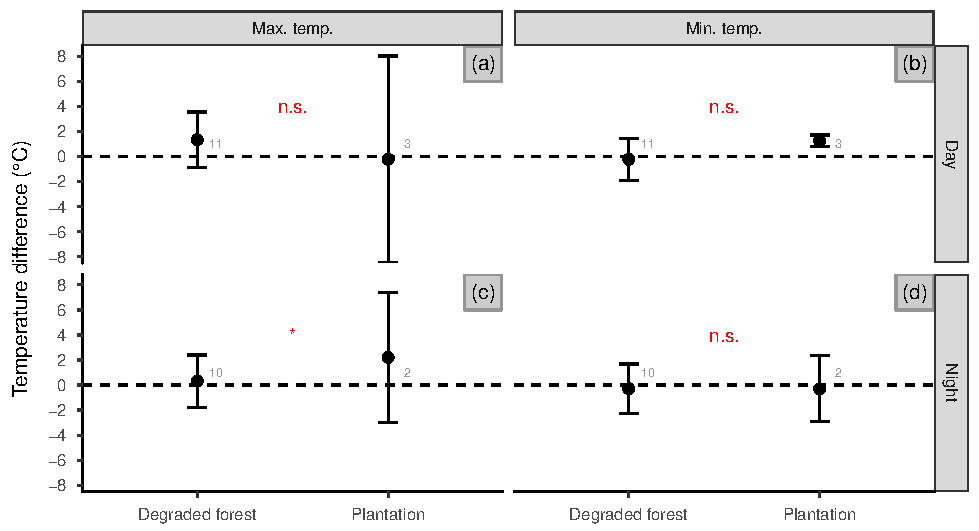
\includegraphics{./output/fig-A-5-1} 

}

\caption{Model estimates of the difference between altered land-use
types and primary forest in terms of temperature extremes. Day-time
results are depicted in panels A and B, and night-time results in panels
C and D. Panels A and C indicate the effect of land-use change on
maximum temperature, and panels B and D indicate the same for minimum
temperature. Note that data for cropland and pasture are absent from
this analysis because data for these land-use types were not available.
Parameter estimates are standardised against the estimate for primary
forest, which is represented by the dotted line. Error bars are 95\%
confidence intervals. The grey numbers next to points represent the
number of studies providing the underlying data.}\label{fig:fig-A-5}
\end{figure}












\begin{figure}[H]

{\centering 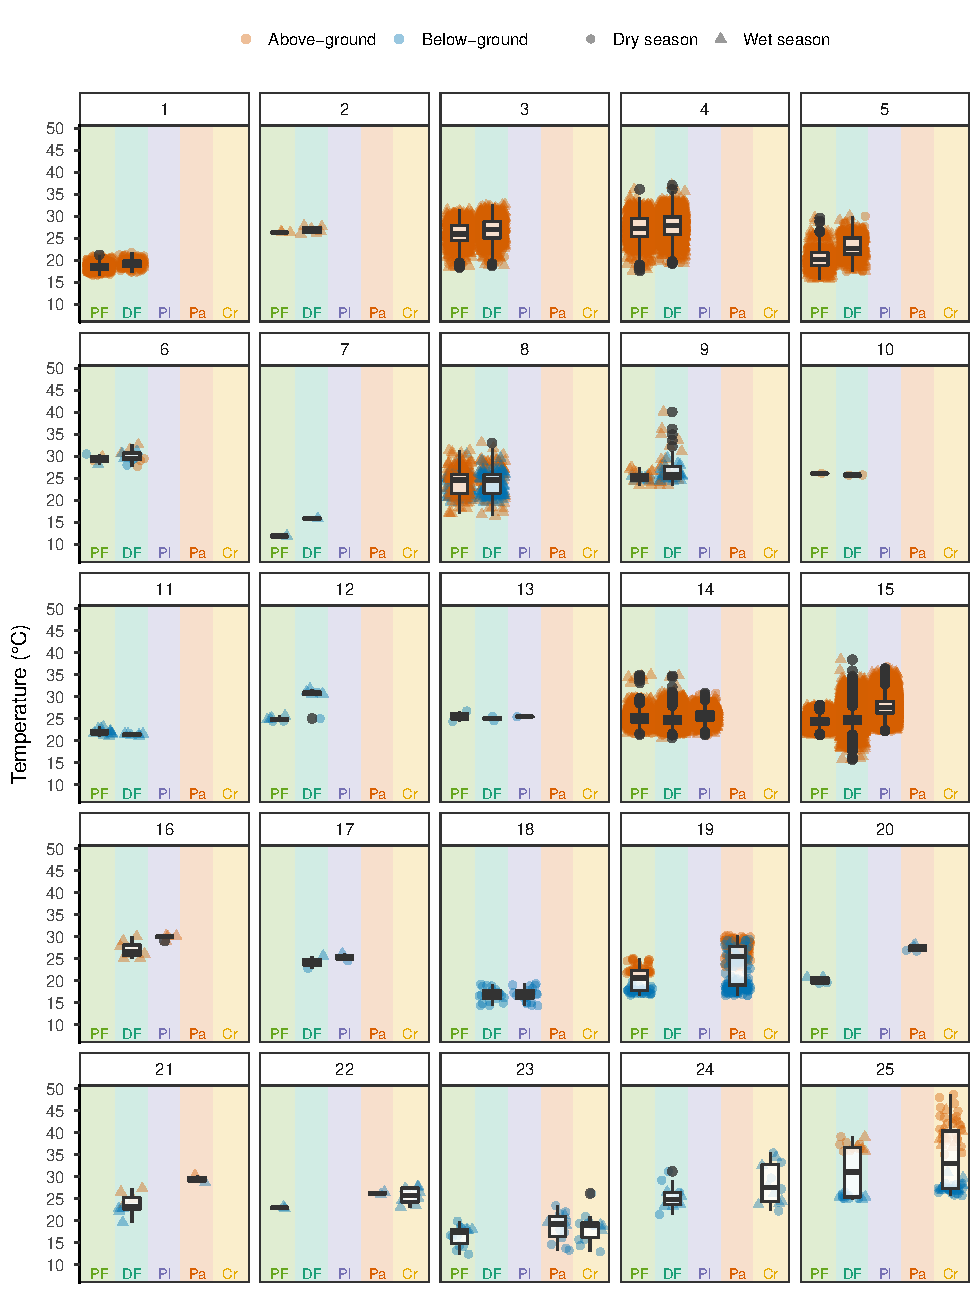
\includegraphics{./output/fig-A-1-1} 

}

\caption{Day-time temperature against land-use type for each study
contributing data to the analyses. Panel numbers refer to the study
number in the reference list below. Land-use types are: primary forest
(PF), degraded forest (DF), plantation (Pl), pasture (Pa) and cropland
(Cr). Panels are ordered by the combination of land-use types for which
data was available: (1-12) PF + DF; (13-15) PF + DF + Pl; (16-18) DF +
Pl; (19-20) PF + Pa; (21) DF + Pa; (22-23) PF + Pa + Cr; and (24-25) DF
+ Cr. Shading of points indicates temperatures measured above-ground
(orange) or below-ground (blue), and point symbol indicates temperatures
measured during the dry season (circles) or wet season (triangles).}\label{fig:fig-A-1}
\end{figure}











\begin{figure}[H]

{\centering 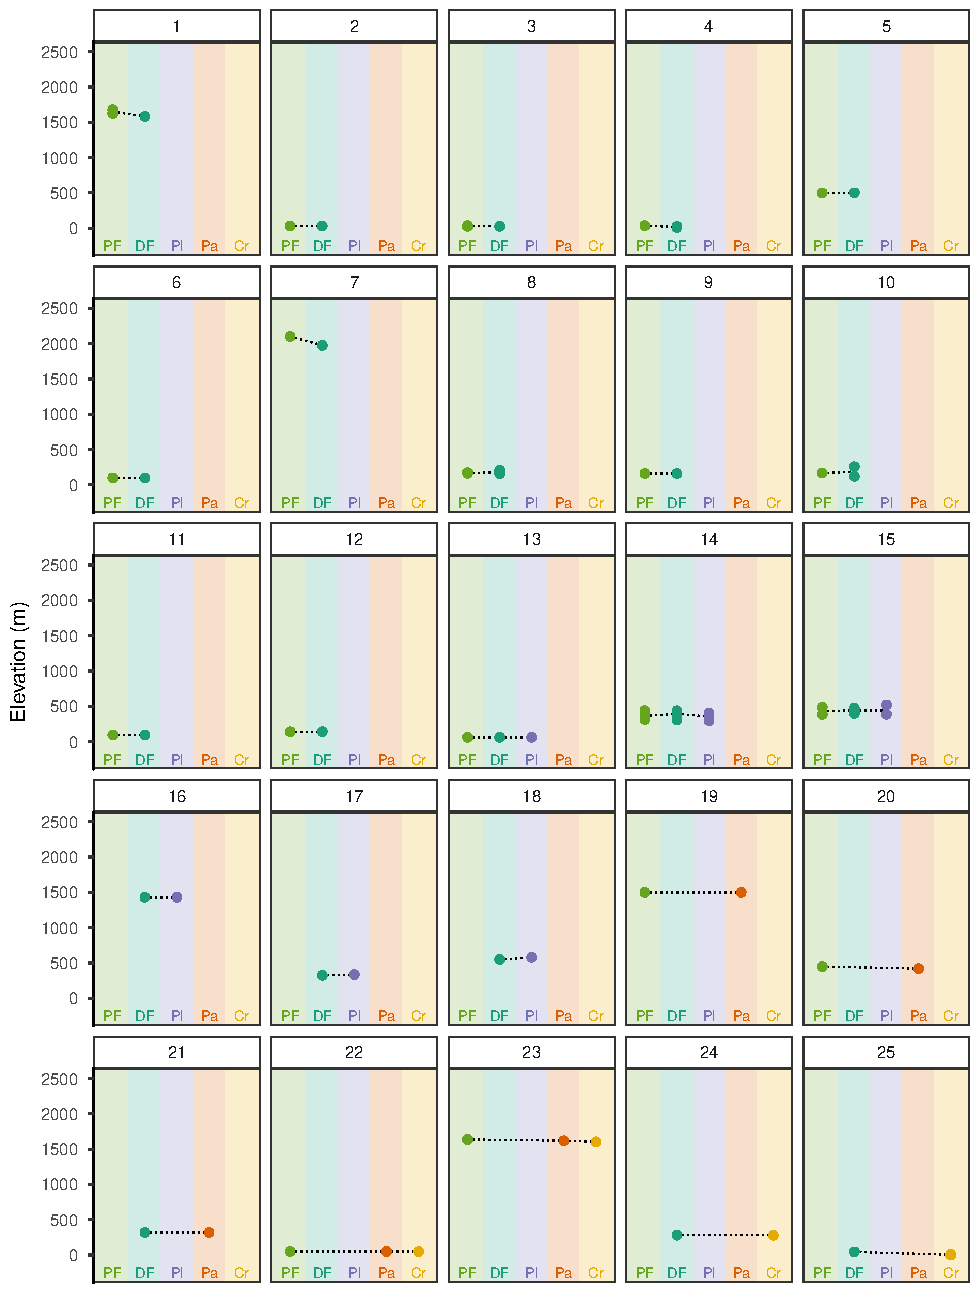
\includegraphics{./output/fig-A-2-1} 

}

\caption{Site elevation against land-use type for each study
contributing data to the analyses. Panel numbers refer to the study
number in the reference list below. Land-use types are: primary forest
(PF), degraded forest (DF), plantation (Pl), pasture (Pa) and cropland
(Cr). Panels are ordered by the combination of land-use types for which
data was available: (1-12) PF + DF; (13-15) PF + DF + Pl; (16-18) DF +
Pl; (19-20) PF + Pa; (21) DF + Pa; (22-23) PF + Pa + Cr; and (24-25) DF
+ Cr. Dotted black lines connect the mean elevation of all the sites
within each land-use type.}\label{fig:fig-A-2}
\end{figure}

\chapter{Supporting information for Chapter
4}\label{supporting-information-for-chapter-4}

\section{Sampling methods for forest structure}\label{text-B-1}

\begin{figure}[H]

{\centering 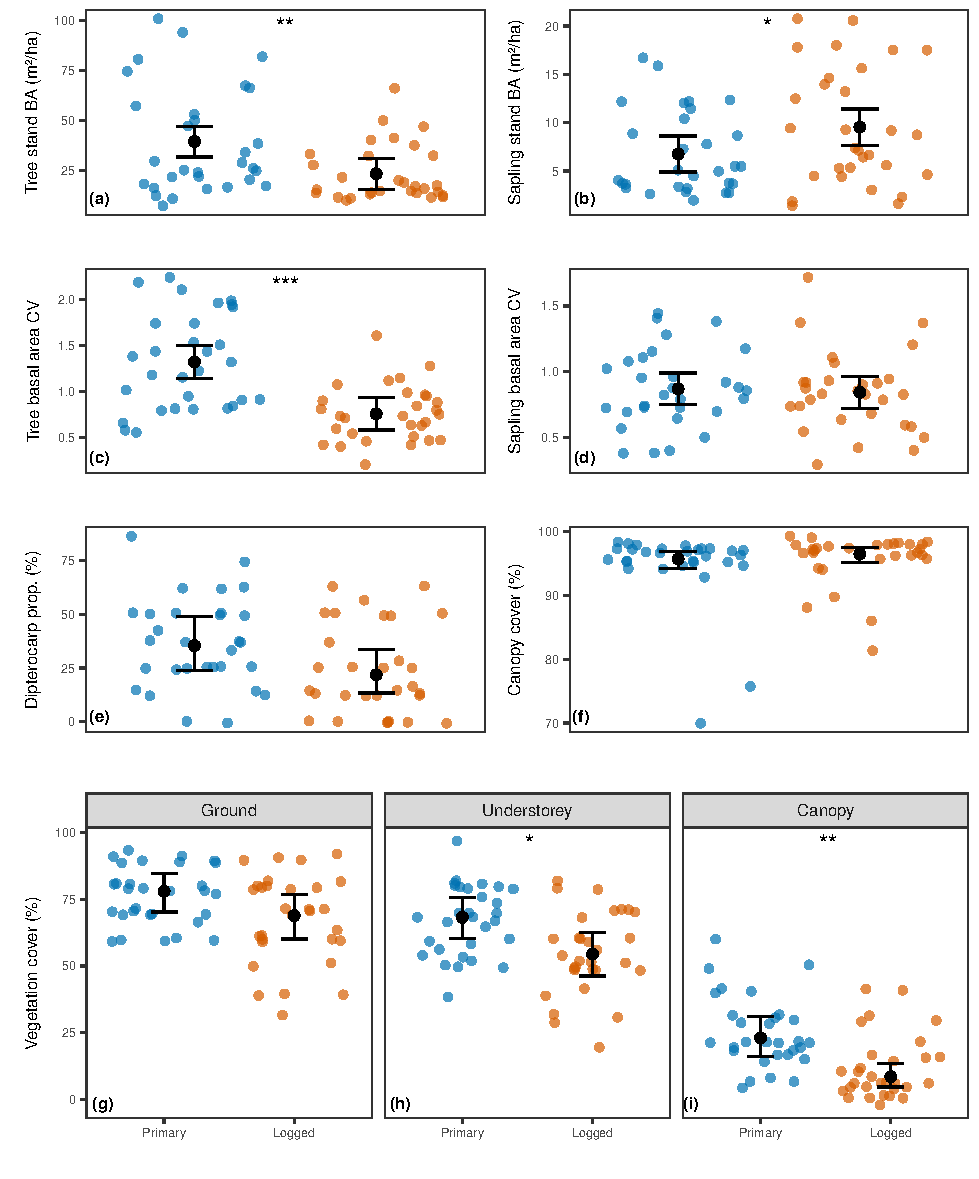
\includegraphics{./output/fig-B-1-1} 

}

\caption{Sampling design schematic.}\label{fig:fig-B-1}
\end{figure}

Several different variables have been previously identified as
efficiently capturing overall forest structure
\citep{hamer_ecology_2003, lucey_spillover_2012}. Each plot (background
circle in the schematic) was divided into quadrants (Q1-Q4). Within each
quadrant we measured the distance to and circumference at breast height
of the two nearest mature trees (circumference \textgreater{} 0.6 m) and
saplings (circumference 0.1-0.6 m). Stand basal area
(m\textsuperscript{2}/ha) was calculated separately for trees and for
saplings. In the above schematic, tree/sapling individuals are depicted
as points: there can be zero, one or two individuals in each quadrant;
the nearest individual is represented by a cross, and the furthest
individual as a star. To estimate stand basal area, we calculated the
basal area of each individual from its circumference at breast height,
summed this across all observed individuals, divided by the true area of
forest that was surveyed and multiplied by 10000 to convert units into
the standard m\textsuperscript{2}/ha. The true area surveyed is depicted
by coloured quadrants; this was calculated for each quadrant
individually and then summed together. Each true quadrant area was
calculated using the equation:

\begin{center}
$A = \frac{1}{4} \pi r^2$
\end{center}

Where A is the area (m\textsuperscript{2}) and r is the distance to the
furthest individual (tree or sapling; m).

To capture plot-level variation in basal area we calculated the
coefficient of variation for trees and for saplings, and we also noted
the proportion of observed tree individuals that were in the family
Dipterocarpaceae, given the association of these species with mature,
complex forest.

Finally, to capture the overall density of vegetation at the plot centre
we measured percentage canopy cover using a spherical densiometer
\citep{lemmon_spherical_1956}, and the same observer estimated
percentage vegetation cover at three distinct forest strata: ground (1.5
m above ground), understorey (15 m above ground) and canopy (the main
mat of leaf cover \textgreater{} 15 m above ground). Visual estimates of
vegetation cover were made by imagining a horizontal gridded plane
intersecting vegetation at the three different heights, and then
estimating the percentage of grid cells occupied by vegetation.

\pagebreak

\section{Extracting and processing data from thermal
images}\label{text-B-2}

Using infrared cameras to sample microclimates in the terrestrial realm
is a relatively novel methodology
\citetext{\citealp{scheffers_extreme_2017}; \citealp[but
see:][]{caillon_warming_2014}; \citealp{faye_toolbox_2016}}. There is,
as yet, no standardised protocol, and there are numerous different
choices of hardware. In this study, we used a FLIR Systems, model E40
camera. A single thermal image comprised 19200 distinct measurements
from the infrared sensor (one per pixel). These raw data can be
extracted and converted to temperature in °C using the freely available
software \href{http://www.flir.com/instruments/display/?id=54865}{FLIR
Tools} \citep[cf.][]{scheffers_extreme_2017}. However, it is easier,
faster and more thorough to use the R package \texttt{Thermimage}
\citep{tattersall_thermimage:_2017}.

Raw data were first extracted from thermal images using the function
\texttt{readflirJPG}, which produces a numeric matrix of the same
dimensions as the original jpeg (160 x 120). The function
\texttt{raw2temp} was then used to convert raw data into temperature
using standard equations from infrared thermography (see
\texttt{?Thermimage::raw2temp} for more details). At this point it is
possible to specify various parameters that likely differ from the
default settings. For emissivity we used a value of 0.986, which
represents the mean of the range (0.982 to 0.990) for bare soil, leaf
litter, live tree leaves and the bark of tree trunks in green broadleaf
forests \citep{snyder_classification-based_1998}. For atmospheric
temperature and relative humidity, we used measurements taken using a
whirling hygrometer immediately prior to each sampling event at each
plot. We defined the distance between the camera and the surface as the
hypotenuse of an isosceles right triangle with its vertical length equal
to breast height: \(1.3\times\sqrt{2} =\) 1.84 m. Finally, there are
five different calibration constants (PlanckR1, PlanckB, PlanckF,
PlanckO and PlanckR2) that are specific to each camera, and we retrieved
these from thermal images using the function \texttt{flirsettings}.

\pagebreak

\section{Sampling methods for microhabitat volume}\label{text-B-3}

We measured the volume of leaf litter in five 1 x 1 m quadrats, centred
2 m to the left of the transect edge, at 0, 10 and 20 m from the plot
centre. Leaf litter was compressed inside a purpose-built compression
cylinder with a plunger, and the volume read directly from a graduated
scale on the cylinder \citep{parsons_volume_2009}.

Within the subplot we measured the length and circumference at both ends
of all intact deadwood (\textgreater{} 10 cm diameter). If only a
portion of the deadwood was contained within the subplot, we measured
that portion only. We calculated volume using Smalian's volume formula
\citep{waddell_sampling_2002}:

\begin{center}
$V = \frac{l \cdot (\frac{\pi}{8}) \cdot (D_S^2 + D_L^2)}{10000}$
\end{center}

Where V is volume (m\textsuperscript{3}), l is the length (m),
D\textsubscript{S} is the small-end diameter (cm), D\textsubscript{L}
the large-end diameter (cm). We also measured the maximum and minimum
diameter of entrances to all tree holes (maximum entrance diameter
\textgreater{} 2 cm and \textless{} 2 m high), and their internal
volume. Approximating the entrance to an ellipse shape, we calculated
entrance area using the standard equation for area of an ellipse:

\begin{center}
$A = \pi \times a \times b$
\end{center}

Where A is entrance area (cm\textsuperscript{2}), a is the maximum
diameter of the entrance (cm) and b is the minimum diameter (cm).
Internal volume could not be adequately measured for one very large tree
hole, hence the plot in which it was located was excluded from analyses.

\pagebreak

\section{Impact of logging on macroclimate}\label{text-B-4}

\subsection{Methods}\label{methods-4}

To interpret the impact of selective logging on thermal buffering by
microclimates in a meaningful way it is also necessary to know whether
macroclimate conditions are affected by selective logging. As discussed
in the Materials and Methods, macroclimate temperature was measured
prior to thermal image collection using a whirling hygrometer, and also
by a temperature datalogger suspended at the centre of each plot (HOBO
pendant datalogger, Onset, model UA-001-64K or model UA-002-64K).

The necessity for thermoregulation, however, is dependent not only on
temperature, but also on water availability. Vapour pressure deficit
(VPD) encompasses both temperature and relative humidity. We measured
VPD in two ways. First, using dry-bulb (i.e.~macroclimate temperature)
and wet-bulb temperature from the whirling hygrometer. We also suspended
one hygrochron iButton datalogger (Maxim, model DS1923) 1.5 m above the
ground in the plot centre of a subset of plots, alongside the HOBO
dataloggers measuring macroclimate temperature. We attempted to
distribute our limited number of hygrochrons as evenly as possible;
ultimately we collected data from 15 plots across all six sites in
primary forest, and from 13 plots across five sites in logged forest. As
there were five plots in each site (Fig. 1), we placed dataloggers
either in plots one, three and five, or plots one and five, depending on
the number of hygrochrons available. Uneven sample sizes resulted
because several hygrochrons were lost or broken. Hygrochrons measured
relative humidity every 20 minutes for six days and, as in the main text
(see Materials and Methods), a unique datapoint was the median value
across each two-hourly increment from 04:40-14:40 hrs, on each day of
recording for each of the 60 total plots.

Macroclimate VPD was calculated from saturated vapour pressure and
relative humidity using the formula:

\begin{center}
$VPD = \frac{100 - RH}{100} \times SVP$
\end{center}

Where VPD is vapour pressure deficit (Pa), RH is relative humidity (\%)
and SVP is saturated vapour pressure (Pa). SVP was calculated from
temperature:

\begin{center}
$SVP = 610.7 \times 10^ \frac{7.5 \times T_d}{237.3 + T_d}$ 
\end{center}

Where T\textsubscript{d} is macroclimate (dry-bulb) temperature (°C).
Relative humidity can be estimated directly from a whirling hygrometer,
but to reduce human error we calculated relative humidity using the
equation:

\begin{center}
$RH = \frac{p}{SVP}$
\end{center}

Where p is partial vapour pressure (Pa), estimated assuming ambient
pressure of 1 atm:

\begin{center}
$p = SVR_w - 66.86 \cdot (1+0.00115 \cdot(T_w)) \cdot (T_d - T_w)$
\end{center}

Where T\textsubscript{d} is dry-bulb temperature (°C),
T\textsubscript{w} is wet-bulb temperature and SVP\textsubscript{w} is
saturated vapour pressure at the wet-bulb temperature, calculated in the
same way as SVP, but substituting in T\textsubscript{w} for
T\textsubscript{d}.

\subsection{Statistical analysis}\label{statistical-analysis-1}

All supplementary analyses were carried out in an analogous way to the
main analyses of microclimate temperature (see Statistical analyses).
The response variables (macroclimate temperature or VPD, from either the
hygrometer or dataloggers) were modelled against the fixed effects
forest quality (measured as tree stand basal area;
m\textsuperscript{2}/ha) and forest type (categorical: primary forest or
logged forest), using linear mixed effects models implemented in the
\texttt{nlme} package \citep{pinheiro_nlme:_2017} in R
\citep{r_core_team_2017}. Plot nested in site was included as a random
intercept term, to account for spatial pseudoreplication. Temporal
autocorrelation of residuals was evident (function \texttt{acf}), and we
therefore included date and time in a correlation structure, with the
best structure determined using AIC \citep{zuur_mixed_2009}. Statistical
significance was inspected using likelihood ratio tests \citep[see
Materials and Methods;][]{zuur_mixed_2009}, and diagnostic plots were
assessed to confirm model fit.

\subsection{Results}\label{results-5}

Macroclimate temperature was comparable between primary and logged
forest whether measured using a whirling hygrometer (LR = 0.081,
\emph{P} = 0.776; Fig. S2a) or suspended datalogger (LR = 0, \emph{P} =
0.983; Fig. S2b), and was also unaffected by forest quality for both the
hygrometer (LR = 0.022, \emph{P} = 0.883; Fig. S2a) and datalogger
measurements (LR = 0.527, \emph{P} = 0.468; Fig. S2b). Similarly,
macroclimate VPD did not differ according to forest type for either
method of VPD measurement: hygrometer (LR = 1.344, \emph{P} = 0.246;
Fig. S2c) and suspended datalogger (LR = 3.489, \emph{P} = 0.062; Fig.
S2d). Neither did the two measures of macroclimate VPD vary with forest
quality (\emph{P} \textgreater{} 0.05; Fig. S2c-d).Thus, we found no
evidence that selective logging impacted macroclimate temperature or
macroclimate VPD.

\pagebreak

\section{Impact of logging on microclimate over 24
hours}\label{text-B-5}

\subsection{Introduction}\label{introduction-4}

We were primarily interested in the impact of selective logging on
thermal buffering at times when buffering from extremes of heat is most
necessary. In the main analyses, therefore, we limited our study to
temperatures recorded between the coolest part of the day (around
sunrise) and the hottest part of the day \citep[around noon;
cf.][]{scheffers_extreme_2017}. However, the wealth of data recorded by
dataloggers also enables us to investigate how thermal buffering varies
over the full 24-hour period, and particularly during the day versus
during the night. In the same way that we would expect logged forests to
receive more incoming solar radiation during the day -- because of
reduced structural complexity and canopy cover
\citep{okuda_effect_2003, kumar_effects_2005} -- we would also expect
these forests to radiate heat more freely at night
\citep{chen_growing-season_1995}. Night-time conditions, although less
thermally challenging, are still important biologically because
nocturnal species can be inactive inside refugia during the heat of the
day, but they must forage and seek mates at night if they are to survive
and reproduce in the long-term.

\subsection{Statistical anlaysis}\label{statistical-anlaysis}

We assessed the impact of selective logging on microclimate temperature
in the same way as in the main text (see Materials and Methods), but
using the full datalogger dataset. Each unique datapoint was the median
of six repeated measures taken every 20 minutes for each two-hourly
interval, for each of six sequential days and in each of the 60 total
plots (5 plots x 12 sites). As these analyses were not compared
alongside results from thermal images, the two-hourly intervals began
from 00:00 hrs (rather than 04:40 hrs). For simplicity, data recorded
between 06:00-18:00 hrs were defined as being during the day, and
18:00-06:00 as during the night. Analyses were carried out separately
for day and night and for each microhabitat: deadwood, tree holes and
leaf litter. Thus, for each analysis (out of six), there was a maximum
of 4320 unique datapoints: 12 time intervals x 6 days x 5 plots x 12
sites.

As in the main text, we used mixed effects models to analyse
microclimate temperature as a function of forest quality (measured as
tree stand basal area; m\textsuperscript{2}/ha), forest type (primary or
logged forest) and macroclimate temperature, with an interaction between
the latter two variables. Models were implemented in the \texttt{nlme}
package \citep{pinheiro_nlme:_2017} in R \citep{r_core_team_2017}. We
included plot nested within site as a random intercept to account for
spatial pseudoreplication, and both date and time in a correlation
structure to account for temporal autocorrelation \citep[the best
structure was determined using AIC;][]{zuur_mixed_2009}. Statistical
significance was inspected using likelihood ratio tests, first dropping
the interaction and comparing to the full model, and then dropping main
effects in turn and comparing to a model without the interaction term
\citep{zuur_mixed_2009}.

\subsection{Results}\label{results-6}

We found no effect of either forest quality or forest type on
microclimates at the surface or inside deadwood and leaf litter
(\emph{P} \textgreater{} 0.05; Fig. S3). We found a very small effect of
both variables on the absolute temperature of microclimates inside tree
holes, during the day. At the median value of tree basal area, tree hole
temperature in primary forest was 24.8°C compared to 24.9°C in logged
forest (LR = 58.202, \emph{P} \textless{} 0.001; Fig. S3b), and with an
increase in forest quality (i.e.~tree stand basal area) of 1
m\textsuperscript{2}/ha, tree hole temperature increased by 0.00504°C
(LR = 57.814, \emph{P} \textless{} 0.001). Evidently, these effects were
extremely small, and therefore unlikely to be relevant to the majority
of organisms.

Similarly, any effects of forest type on the relationship between
microclimate and macroclimate temperature, while statistically
significant, were small in real terms. During the day, 1°C of warming in
the macroclimate (from its median temperature) corresponded to more
warming in primary forest than in logged forest for tree holes (LR =
18.214, \emph{P} \textless{} 0.001; Fig. S3b) and leaf litter (LR =
40.957, \emph{P} \textless{} 0.001; Fig. S3c), but there was no
difference for microclimates inside deadwood (LR = 0.254, \emph{P} =
0.614; Fig. S3a). At night, 1°C of cooling in the macroclimate
corresponded to more cooling in primary forest than in logged forest for
microclimates inside deadwood (LR = 8.589, \emph{P} \textless{} 0.01;
Fig. S3d) and leaf litter (LR = 861.623, \emph{P} \textless{} 0.001;
Fig. S3f), but there was no longer any observed difference for
microclimates inside tree holes (LR = 1.359, \emph{P} = 0.244; Fig.
S3e).

Overall, there is some evidence that thermal buffering from warming and
cooling is slightly enhanced for microclimates in logged forest compared
to primary forest, but in reality the size of these effects was so small
that they are unlikely to have much biological relevance. This is also
evident from the large confidence intervals of Fig. S4, which
demonstrate that for most values of macroclimate temperature, primary
and logged forests did not differ in microclimate temperature.

\pagebreak

\section{Supplementary figures}\label{supplementary-figures-1}










\begin{figure}[H]

{\centering 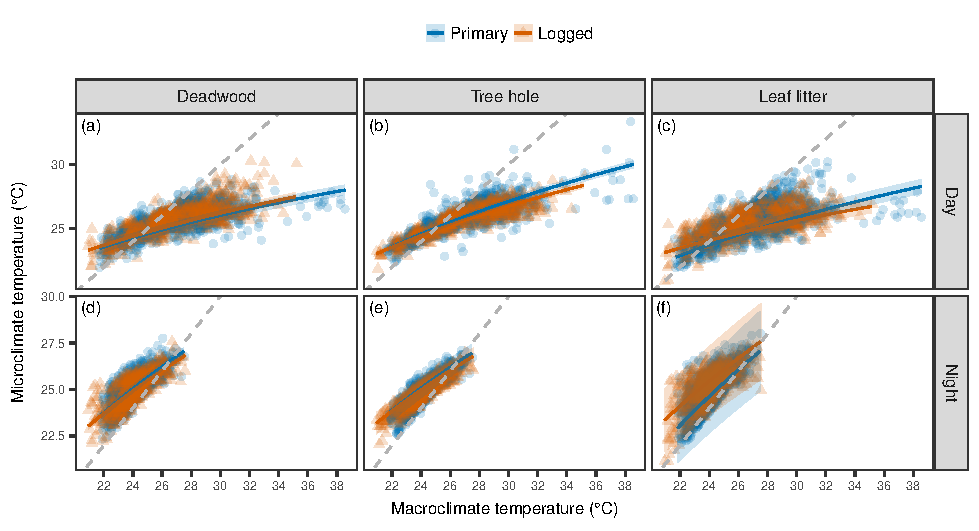
\includegraphics{./output/fig-B-3-1} 

}

\caption{The influence of forest type (primary or logged forest)
and forest quality (measured as tree stand basal area;
m\textsuperscript{2}/ha) on macroclimate temperature (top row) and
macroclimate vapour pressure deficit (VPD; bottom row). Macroclimate
measurements collected using a whirling hygrometer are shown in the left
column, and from dataloggers in the right column. Datapoints from
primary forest points are depicted as blue circles, and from logged
forest as orange triangles. Shaded bands are 95\% confidence intervals.}\label{fig:fig-B-3}
\end{figure}










\begin{figure}[H]

{\centering 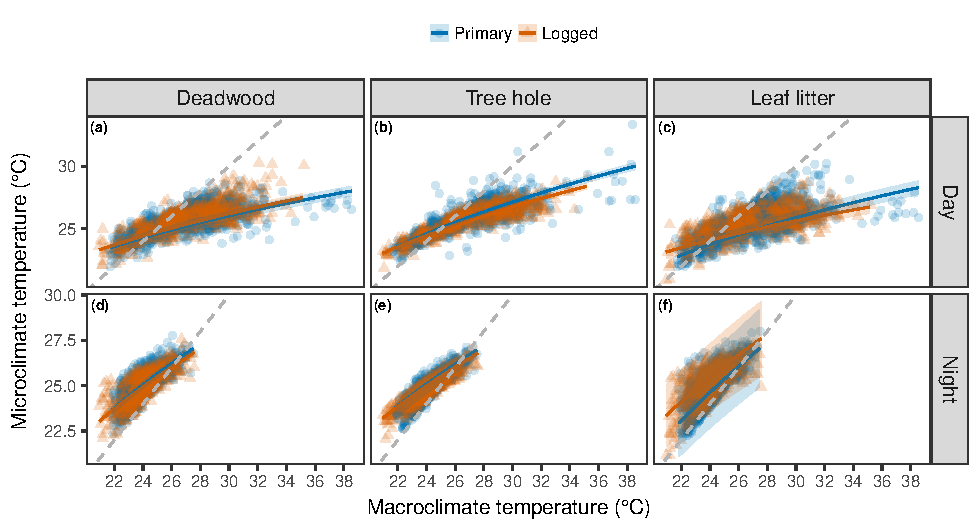
\includegraphics{./output/fig-B-4-1} 

}

\caption{Comparison of the relationship between microclimate
temperature and macroclimate temperature within primary forest (blue
circles) and logged forest (orange triangles), during the day (top row)
and night (bottom row), and for three microhabitats: deadwood (left
column), tree holes (centre column) and leaf litter (right column). The
grey dashed line indicates zero temperature buffering, where the
microclimate temperature is equal to the macroclimate temperature.
Shaded bands are 95\% confidence intervals.}\label{fig:fig-B-4}
\end{figure}













\begin{figure}[H]

{\centering 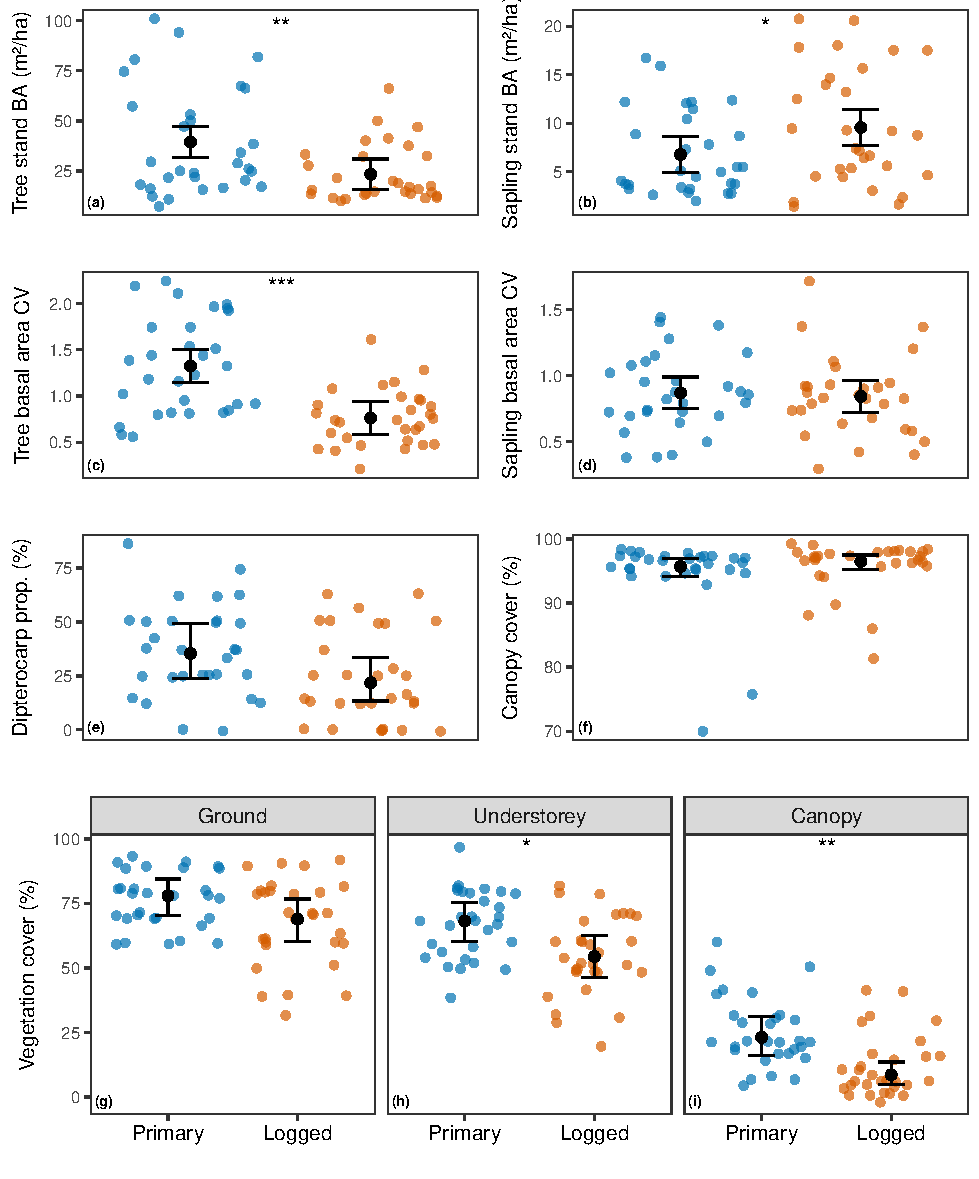
\includegraphics{./output/fig-B-2-1} 

}

\caption{Comparison between primary forest (blue) and logged forest
(orange) for the nine forest structure measures: the stand basal area of
trees (a) and saplings (b); the coefficient of variation for tree basal
area (c) and sapling basal area (d); the proportion of trees that were
in the family Dipterocarpaceae (e); the percentage canopy cover (f); and
visual estimates of percentage vegetation at 1.5 m above ground (g), 15
m above ground (h) and \textgreater{} 15 m above ground (i).
Statistically significant differences are indicated by asterisks,
differentiating between: 0.01 \textless{} \emph{P} \textless{} 0.05 (*);
0.001 \textless{} \emph{P} \textless{} 0.01 (**) and \emph{P}
\textless{} 0.0001 (***). Error bars are 95\% confidence intervals.}\label{fig:fig-B-2}
\end{figure}

\clearpage
\fancyhead[R]{Bibliography}

\bibliography{refs.bib,funky-refs.bib}


\end{document}
